%
% Chapter 9
%

\chapter{Results}
\label{results}

After applying the selection criteria, the expected limits are calculated from a final discrimination variable using the profile likelihood method with asymptotic approximation. Two different fits are considered, with differences in the discrimination variable employed and changes to the selection. The primary results are obtained from a fit to the BDT discriminator after the preselection. The cross-check results are obtained from a fit to the \mcol distribution after applying stringent selection criteria. The fits are performed per channel and category and then combined to set 95\% CL upper limits on the branching fraction of LFV Higgs decay in the \Hmt and \Het channels, \BHmt, and \BHet, respectively. The BDT discriminator distributions of signal and background for each category for \Hmt and \Het can be seen in Figures~\ref{fig:bdt_muhad},~\ref{fig:bdt_mue},~\ref{fig:bdt_ehad}, and~\ref{fig:bdt_emu} respectively. The $\mcol$ discriminator distributions of signal and background for each category for \Hmt and \Het can be seen in Figures~\ref{fig:mcol_muhad},~\ref{fig:mcol_mue},~\ref{fig:mcol_ehad}, and~\ref{fig:mcol_emu} respectively.

\begin{figure}[htbp!]
  \centering
  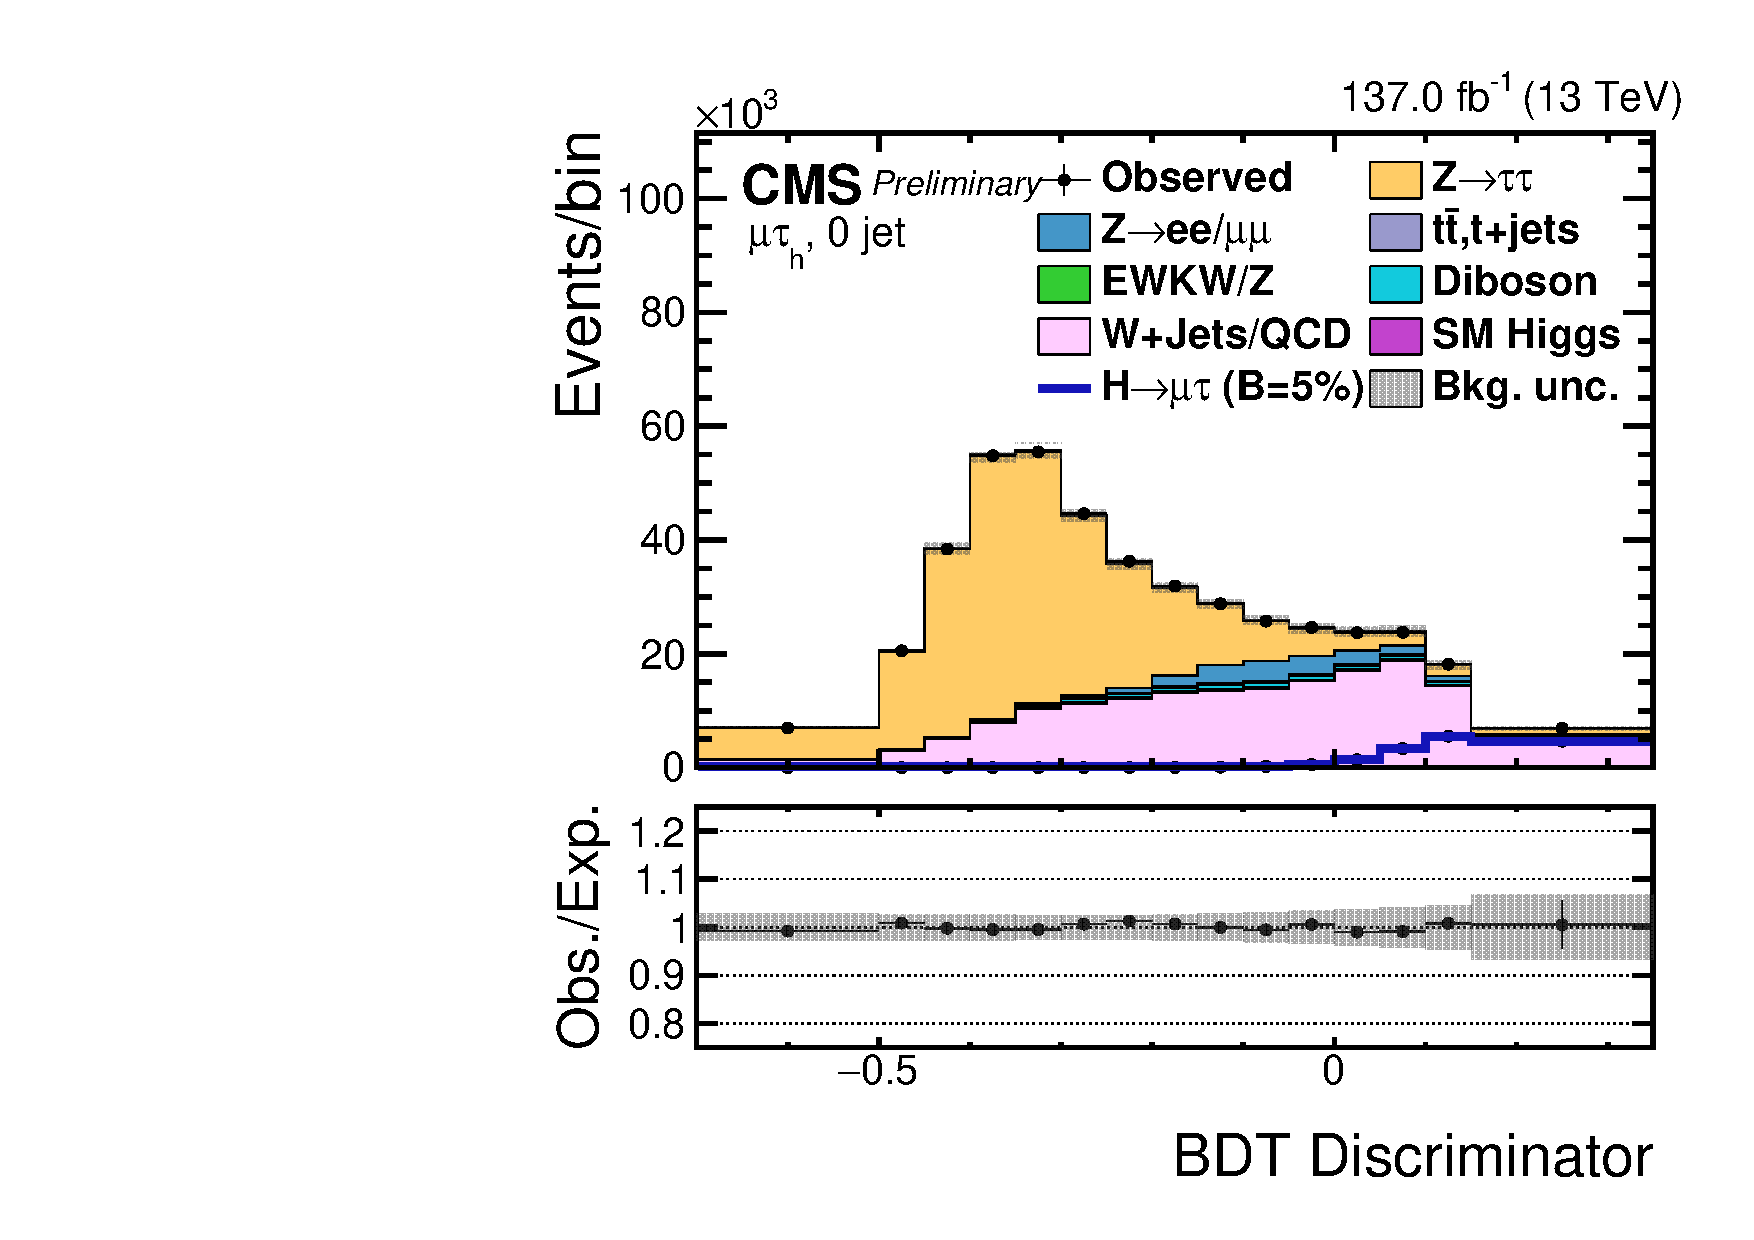
\includegraphics[width=0.4\textwidth]{plots/chapter9/BDT/mutau/0jet.pdf}
  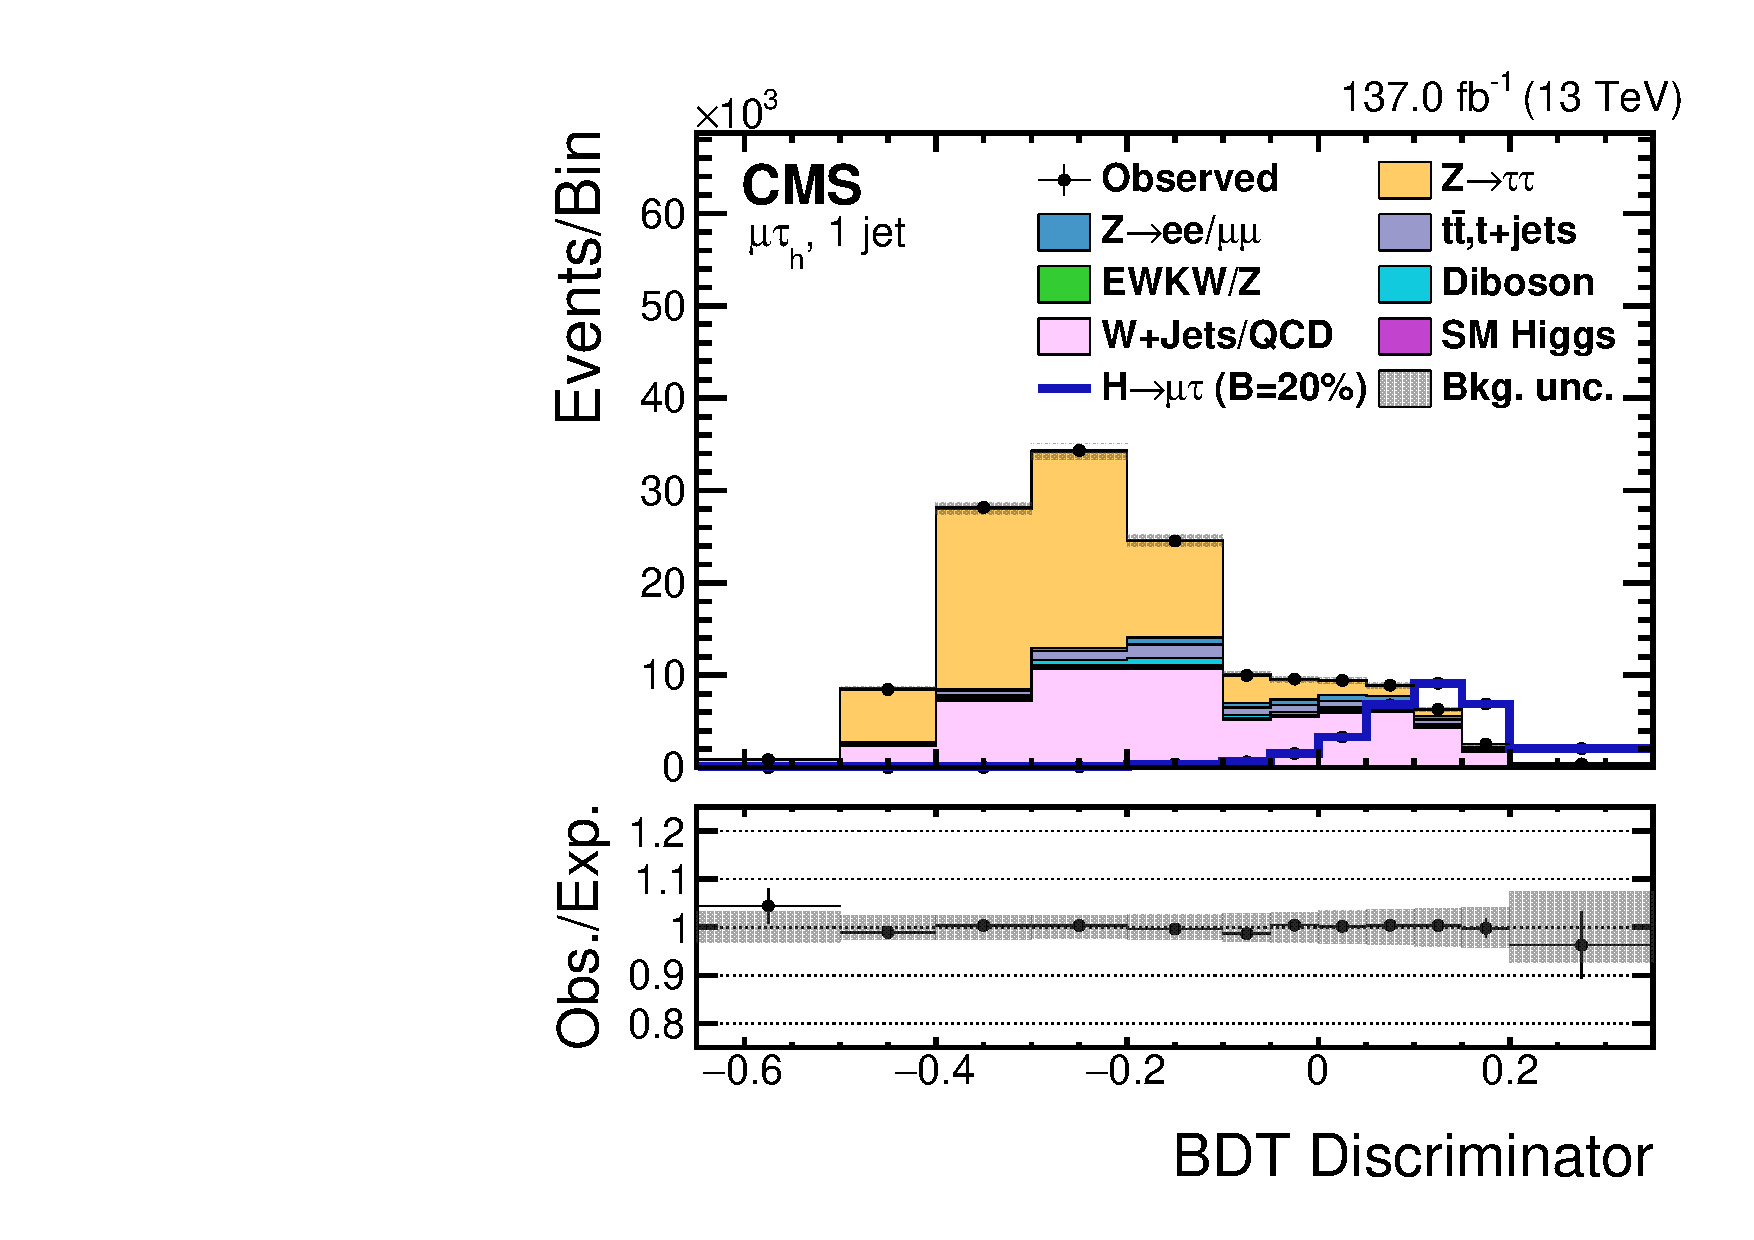
\includegraphics[width=0.4\textwidth]{plots/chapter9/BDT/mutau/1jet.pdf} \\
  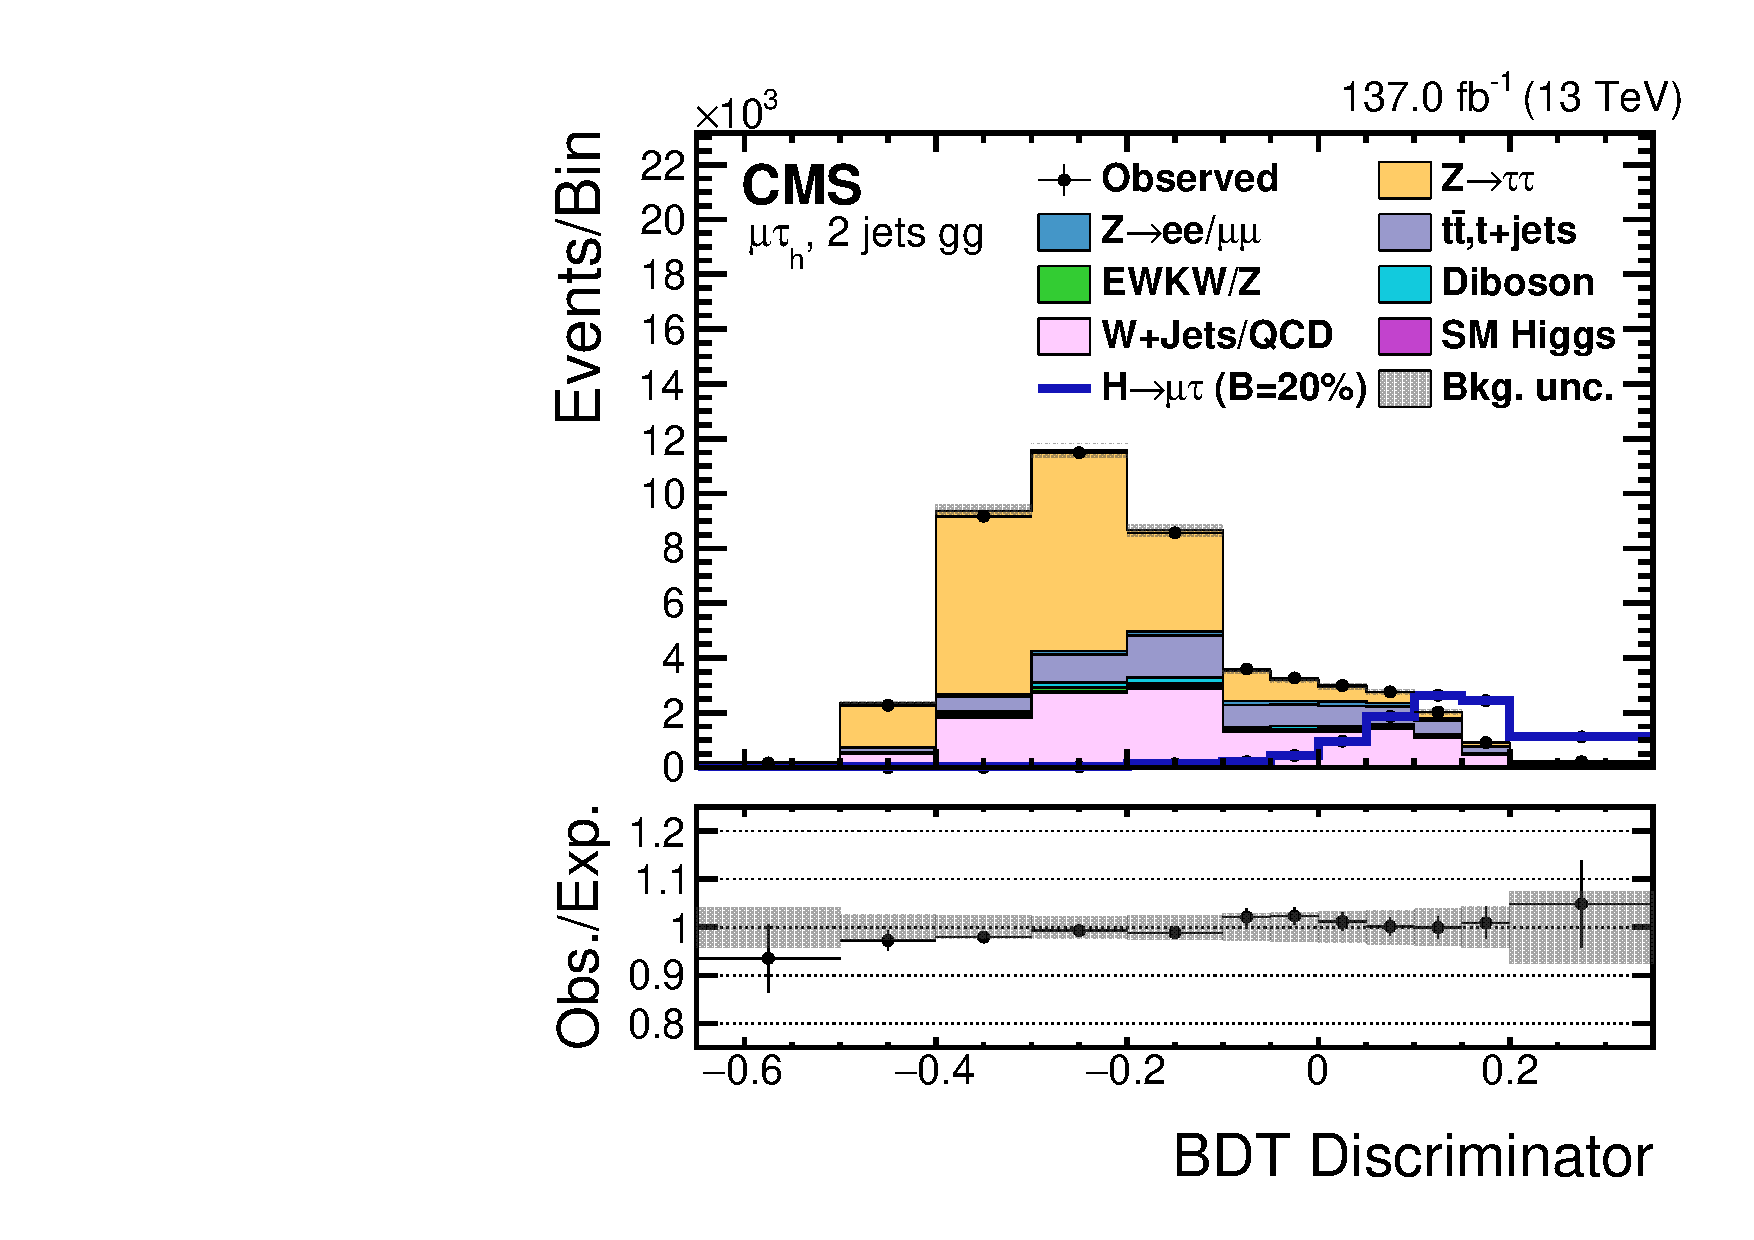
\includegraphics[width=0.4\textwidth]{plots/chapter9/BDT/mutau/2jet_gg.pdf}
  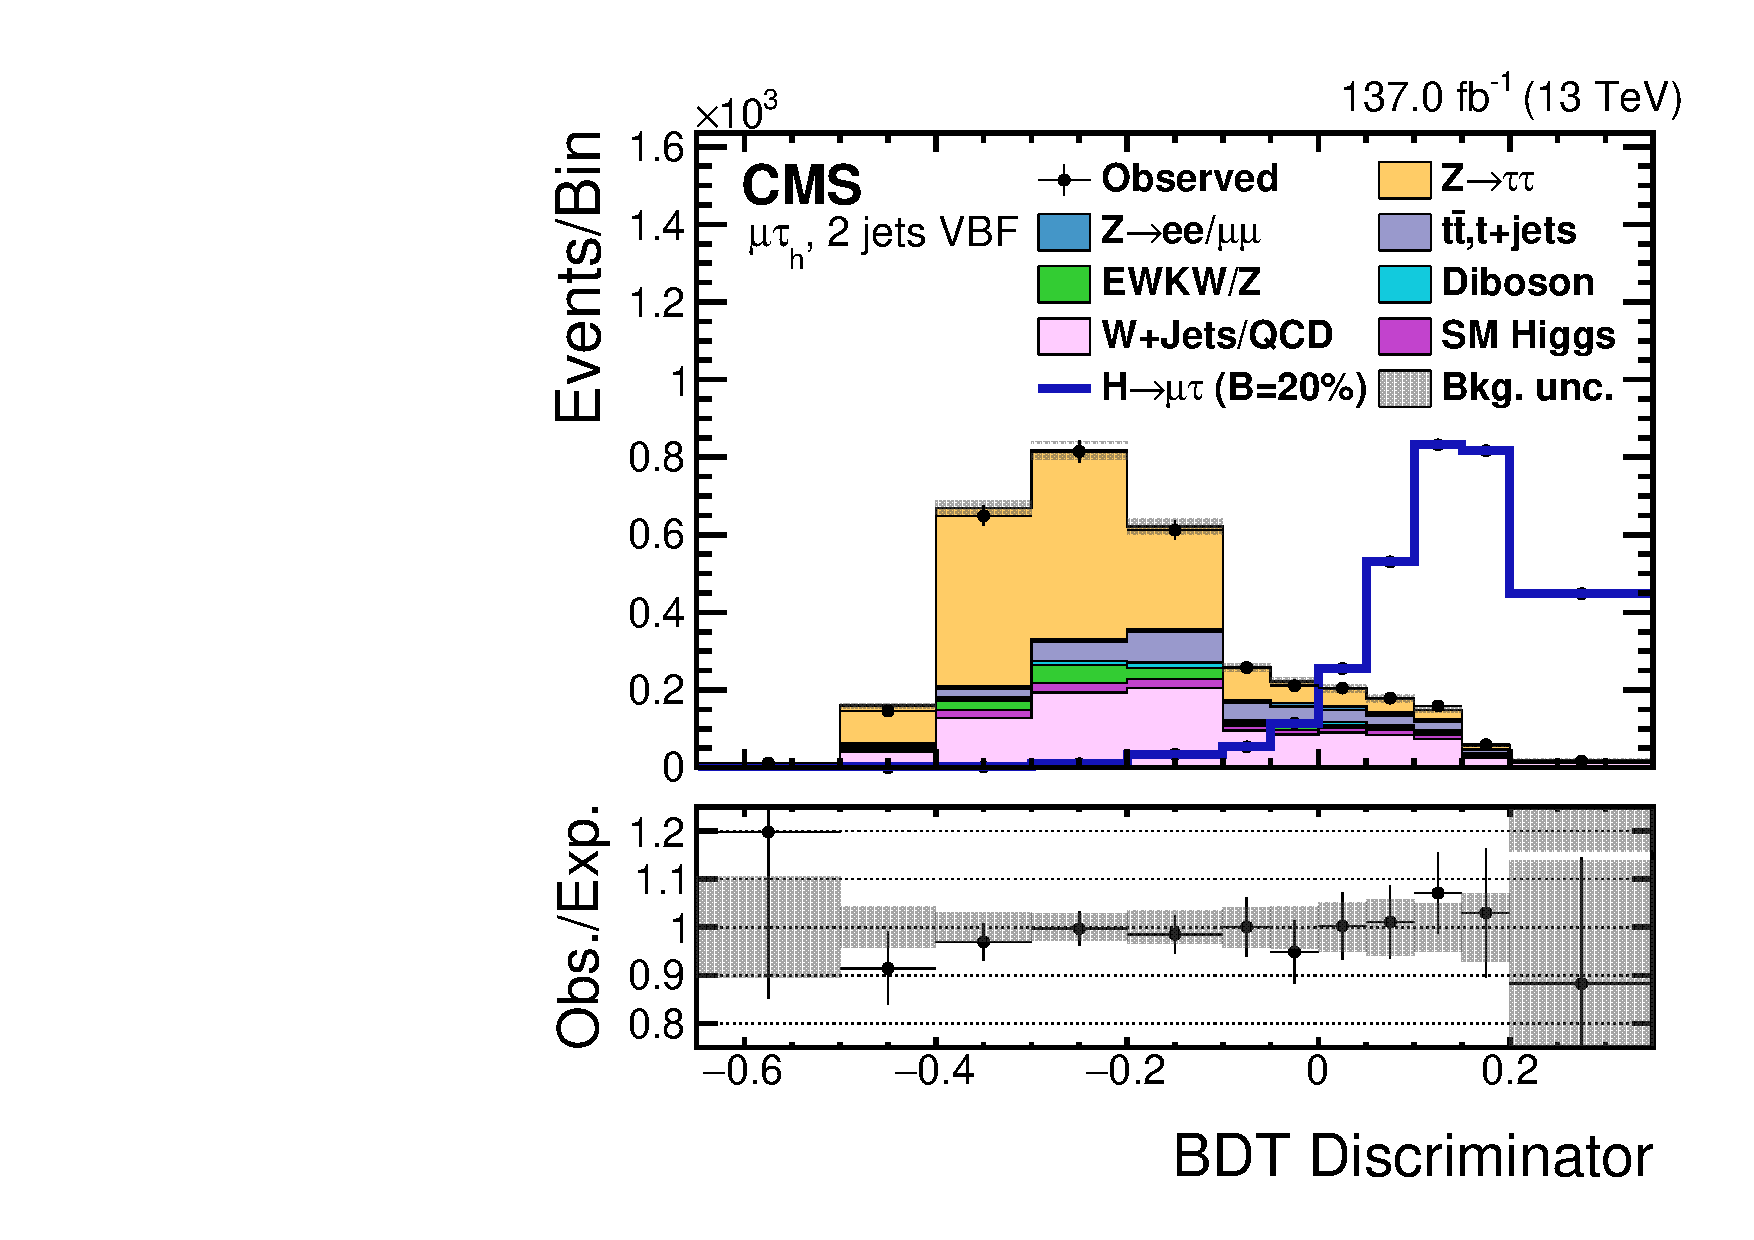
\includegraphics[width=0.4\textwidth]{plots/chapter9/BDT/mutau/2jet_vbf.pdf} \\
  \caption{BDT discriminator distributions for the observed and estimated background in the \muhad channel. The background is normalized to the best fit values from the signal plus background fit. Signal corresponds to \BHmt = 20\%. The \muhad channel categories are 0 jets (top left), 1 jet (top right), 2 jets gg (bottom left), and 2 jets VBF (bottom right). The bottom panel in each plot shows the fractional difference between the observed and estimated background. The uncertainty band shows the statistical and systematic uncertainties added in quadrature.}
  \label{fig:bdt_muhad}
\end{figure}

\begin{figure}[htbp!]
  \centering
  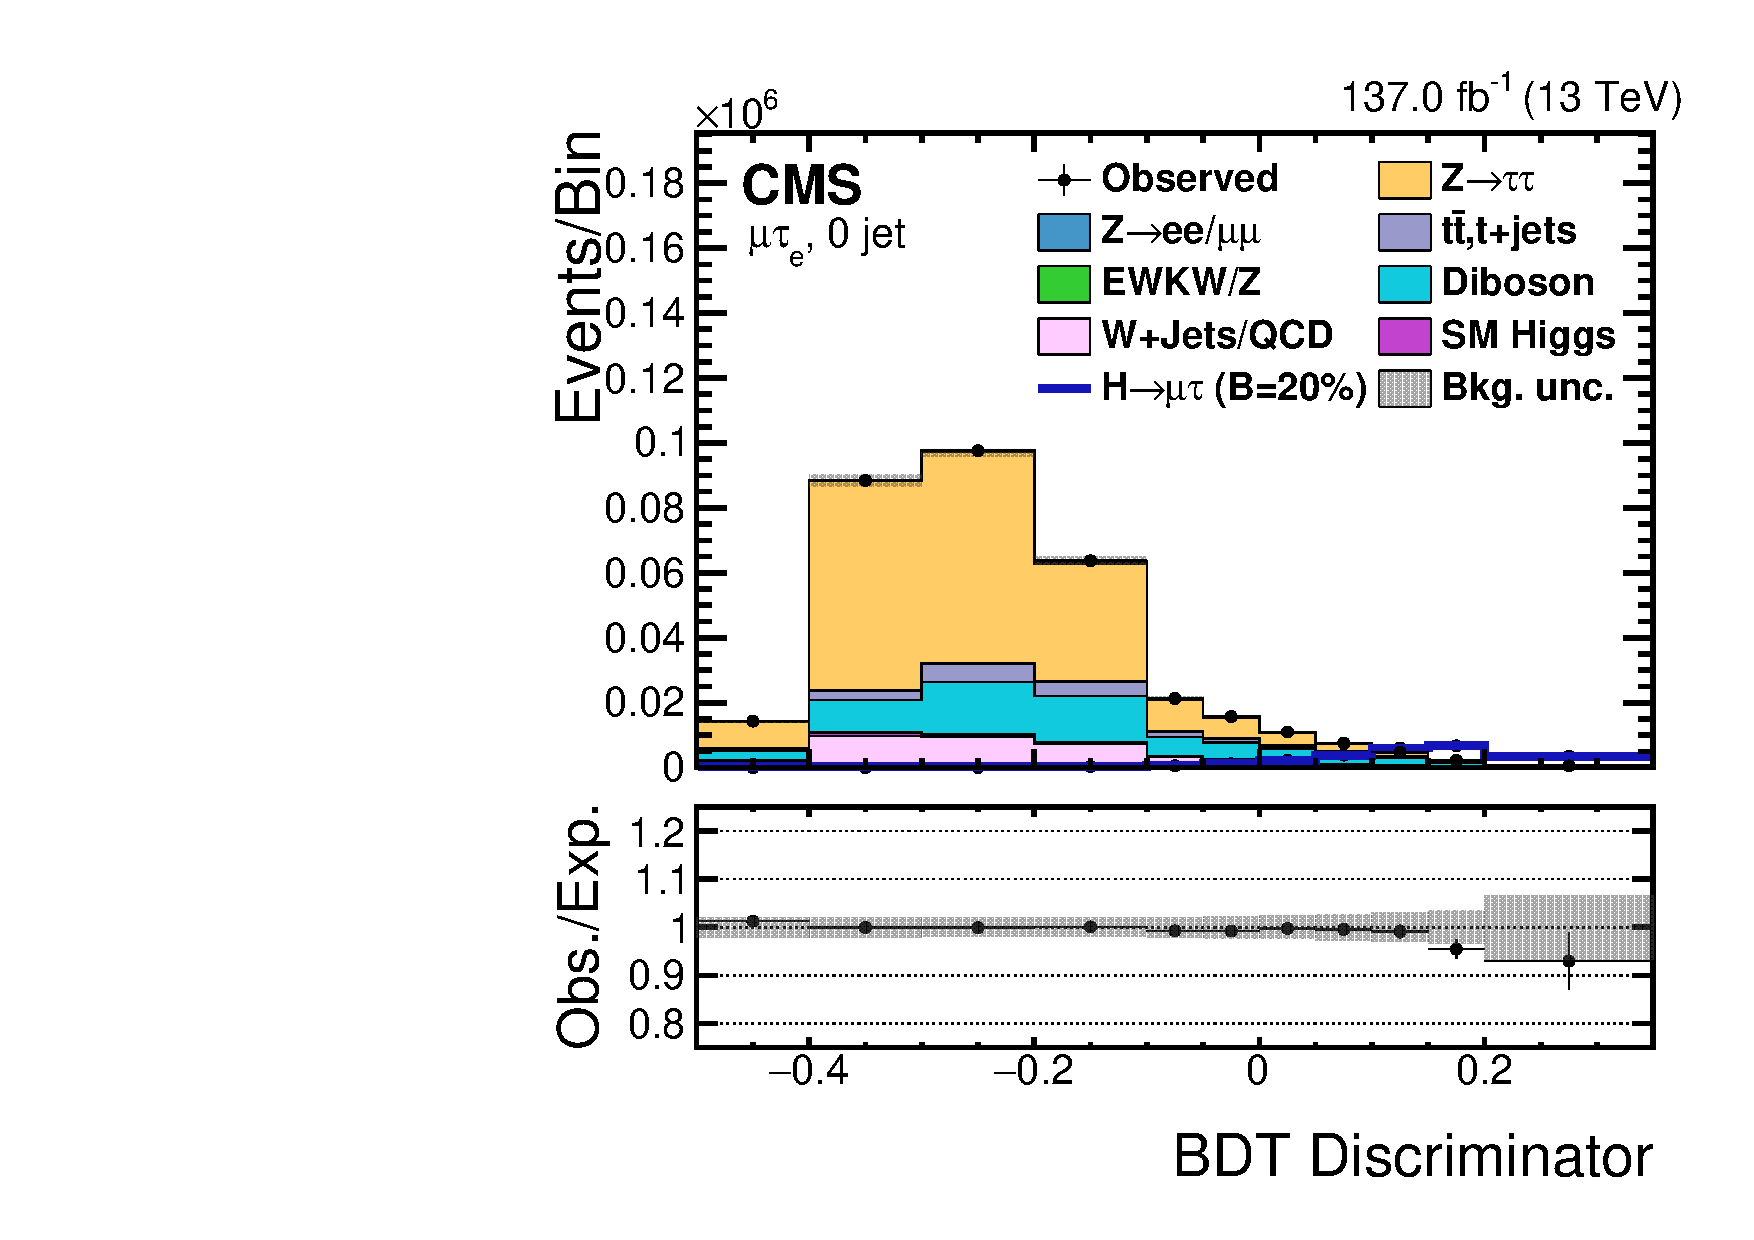
\includegraphics[width=0.4\textwidth]{plots/chapter9/BDT/mue/0jet.pdf}
  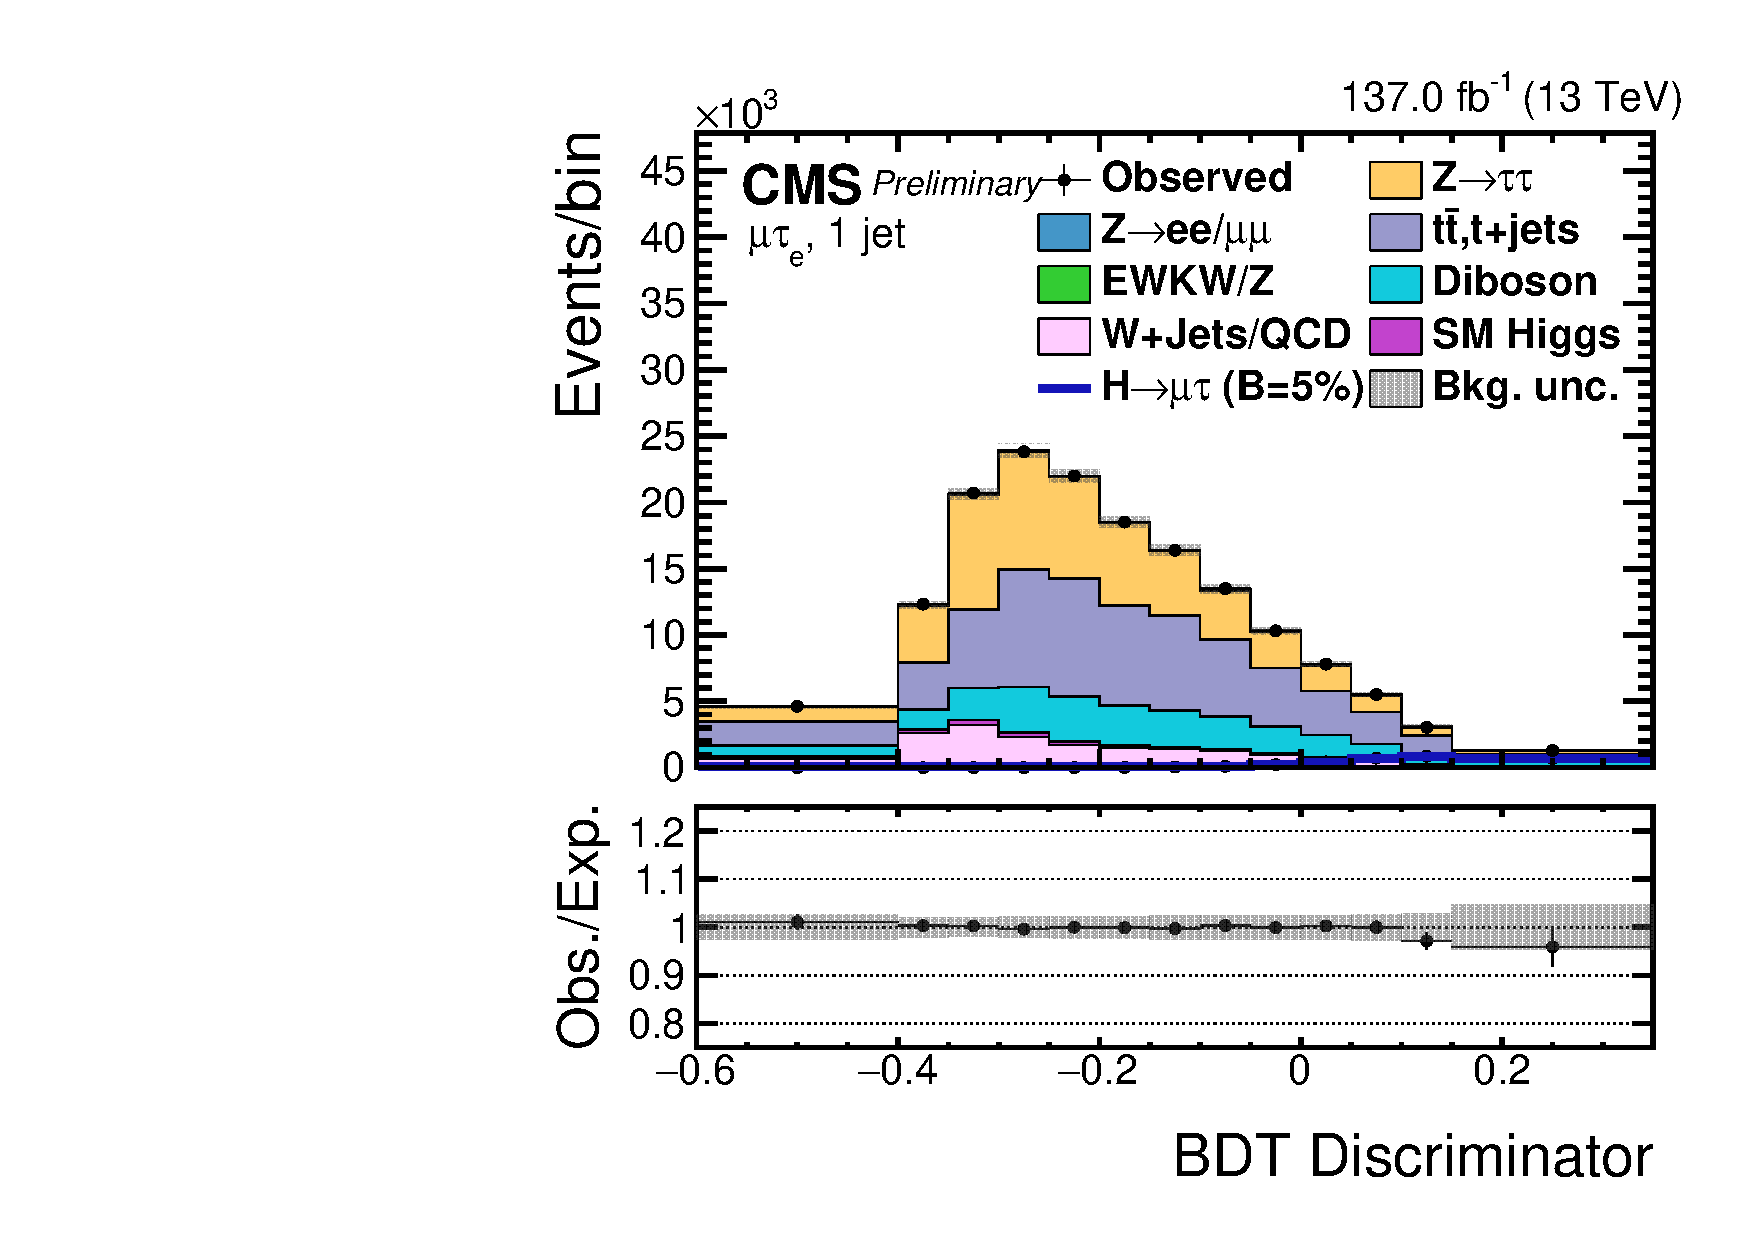
\includegraphics[width=0.4\textwidth]{plots/chapter9/BDT/mue/1jet.pdf} \\
  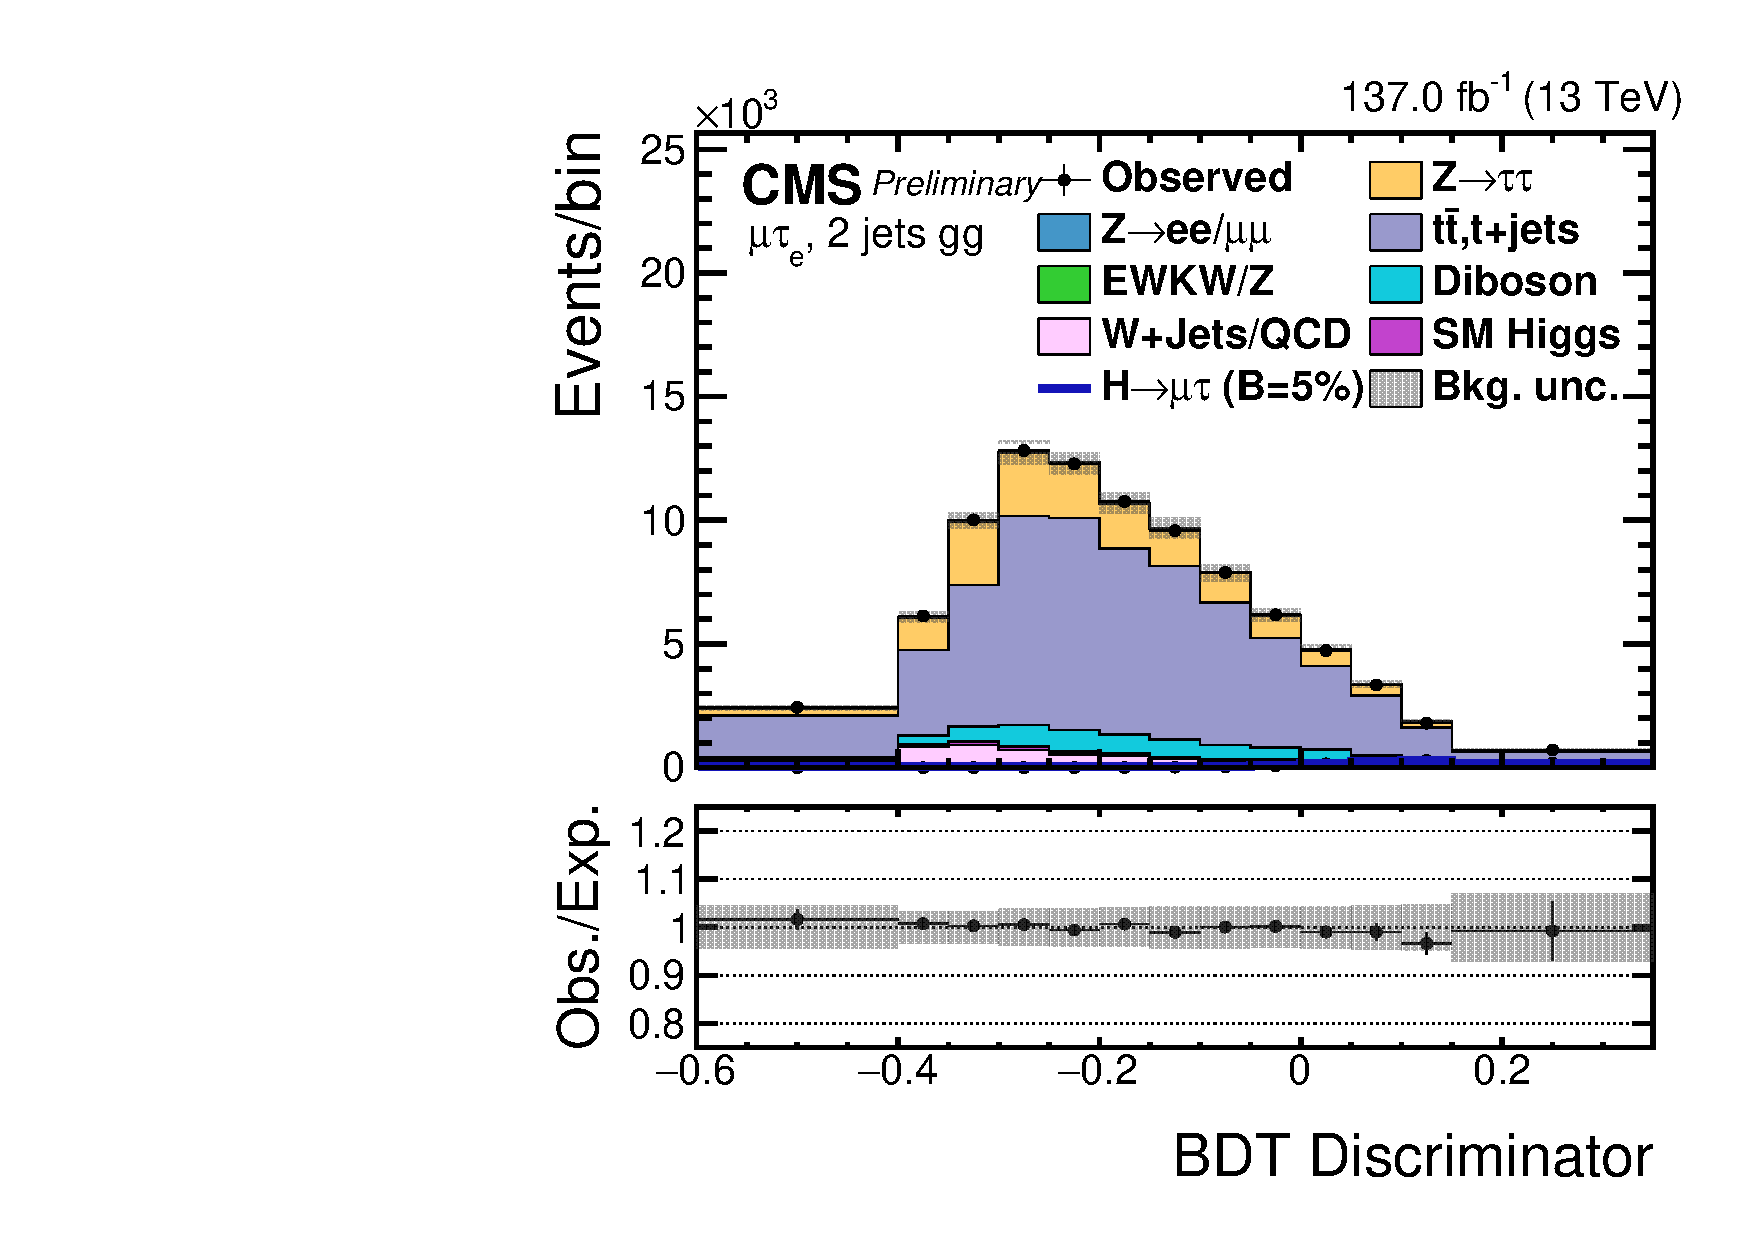
\includegraphics[width=0.4\textwidth]{plots/chapter9/BDT/mue/2jet_gg.pdf}
  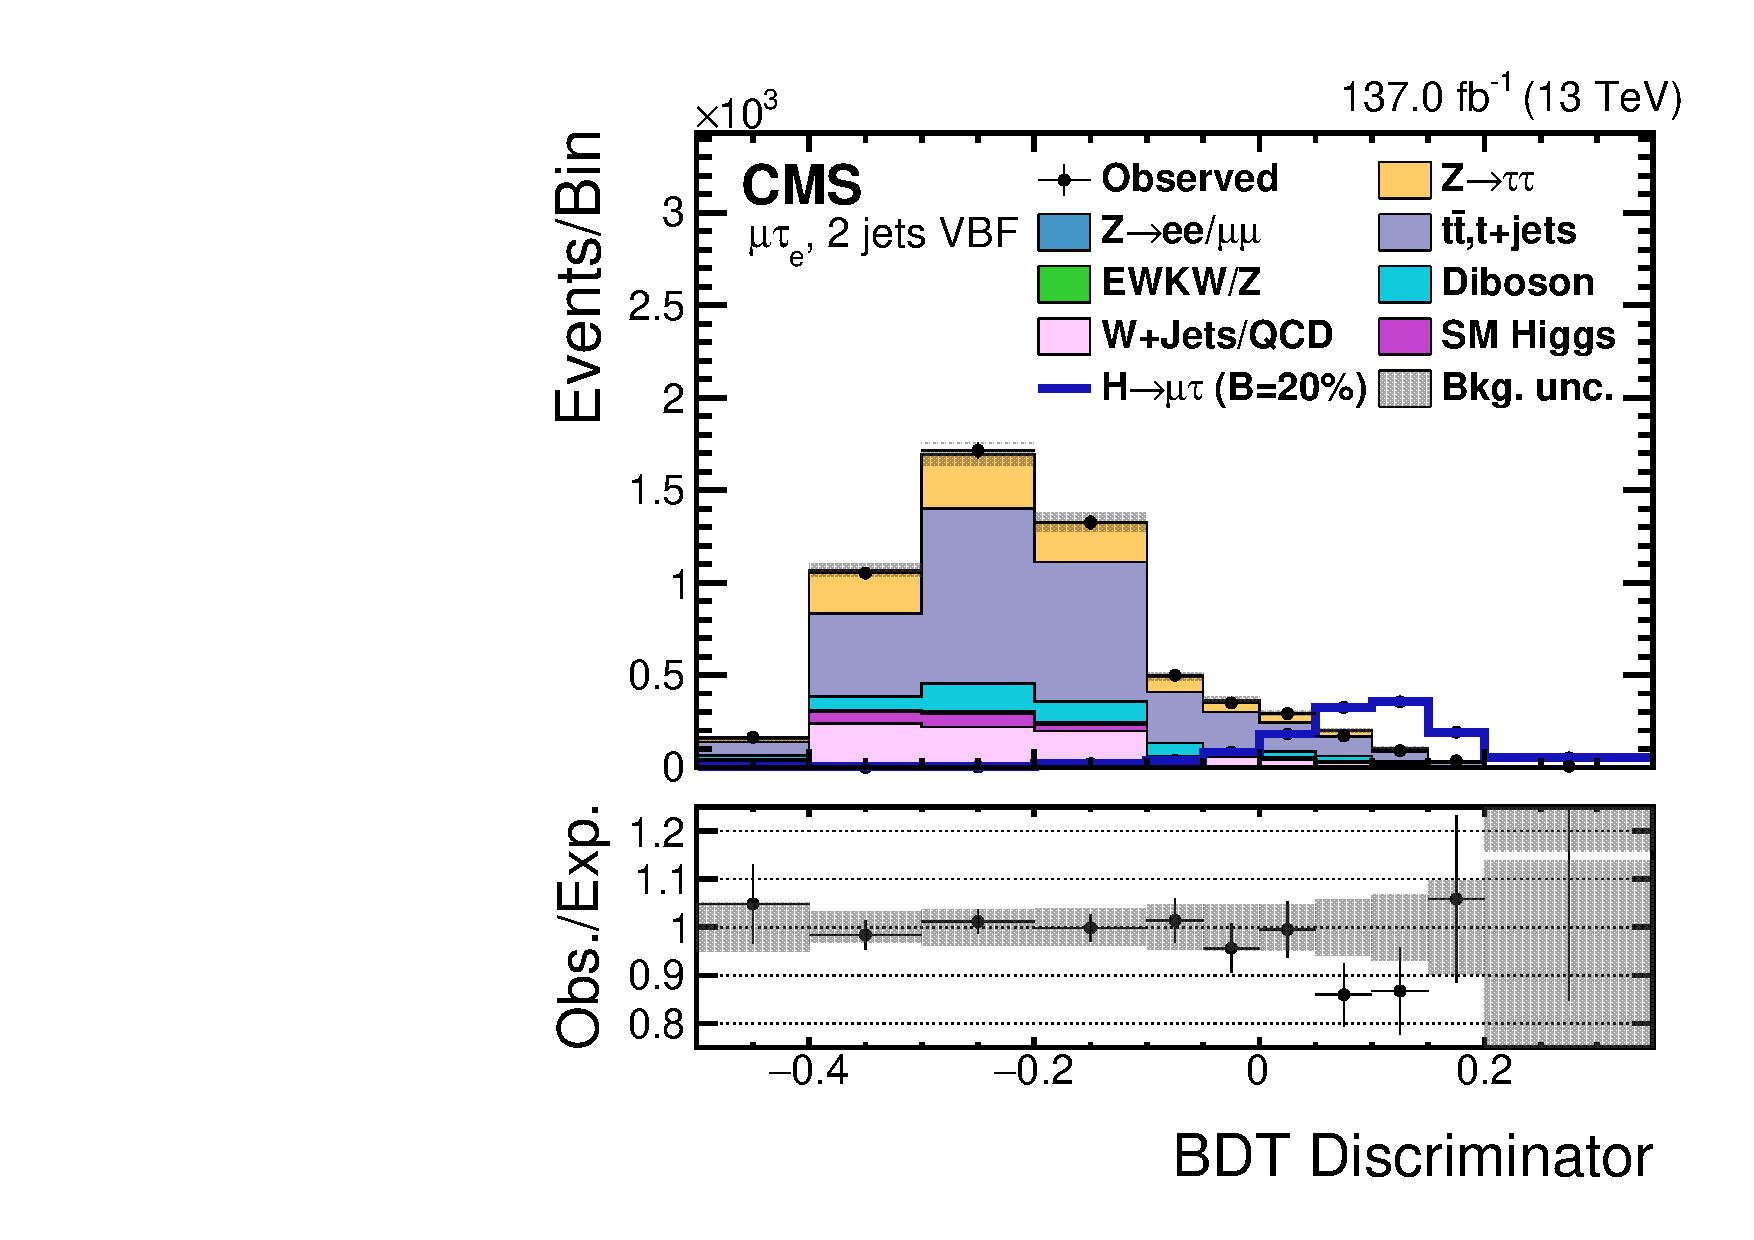
\includegraphics[width=0.4\textwidth]{plots/chapter9/BDT/mue/2jet_vbf.pdf} \\
  \caption{BDT discriminator distributions for the observed and estimated background in the \mue channel. The background is normalized to the best fit values from the signal plus background fit. Signal corresponds to \BHmt = 20\%. The \mue channel categories are 0 jets (top left), 1 jet (top right), 2 jets gg (bottom left), and 2 jets VBF (bottom right). The bottom panel in each plot shows the fractional difference between the observed and estimated background. The uncertainty band shows the statistical and systematic uncertainties added in quadrature.}
  \label{fig:bdt_mue}
\end{figure}

\begin{figure}[htbp!]
  \centering
  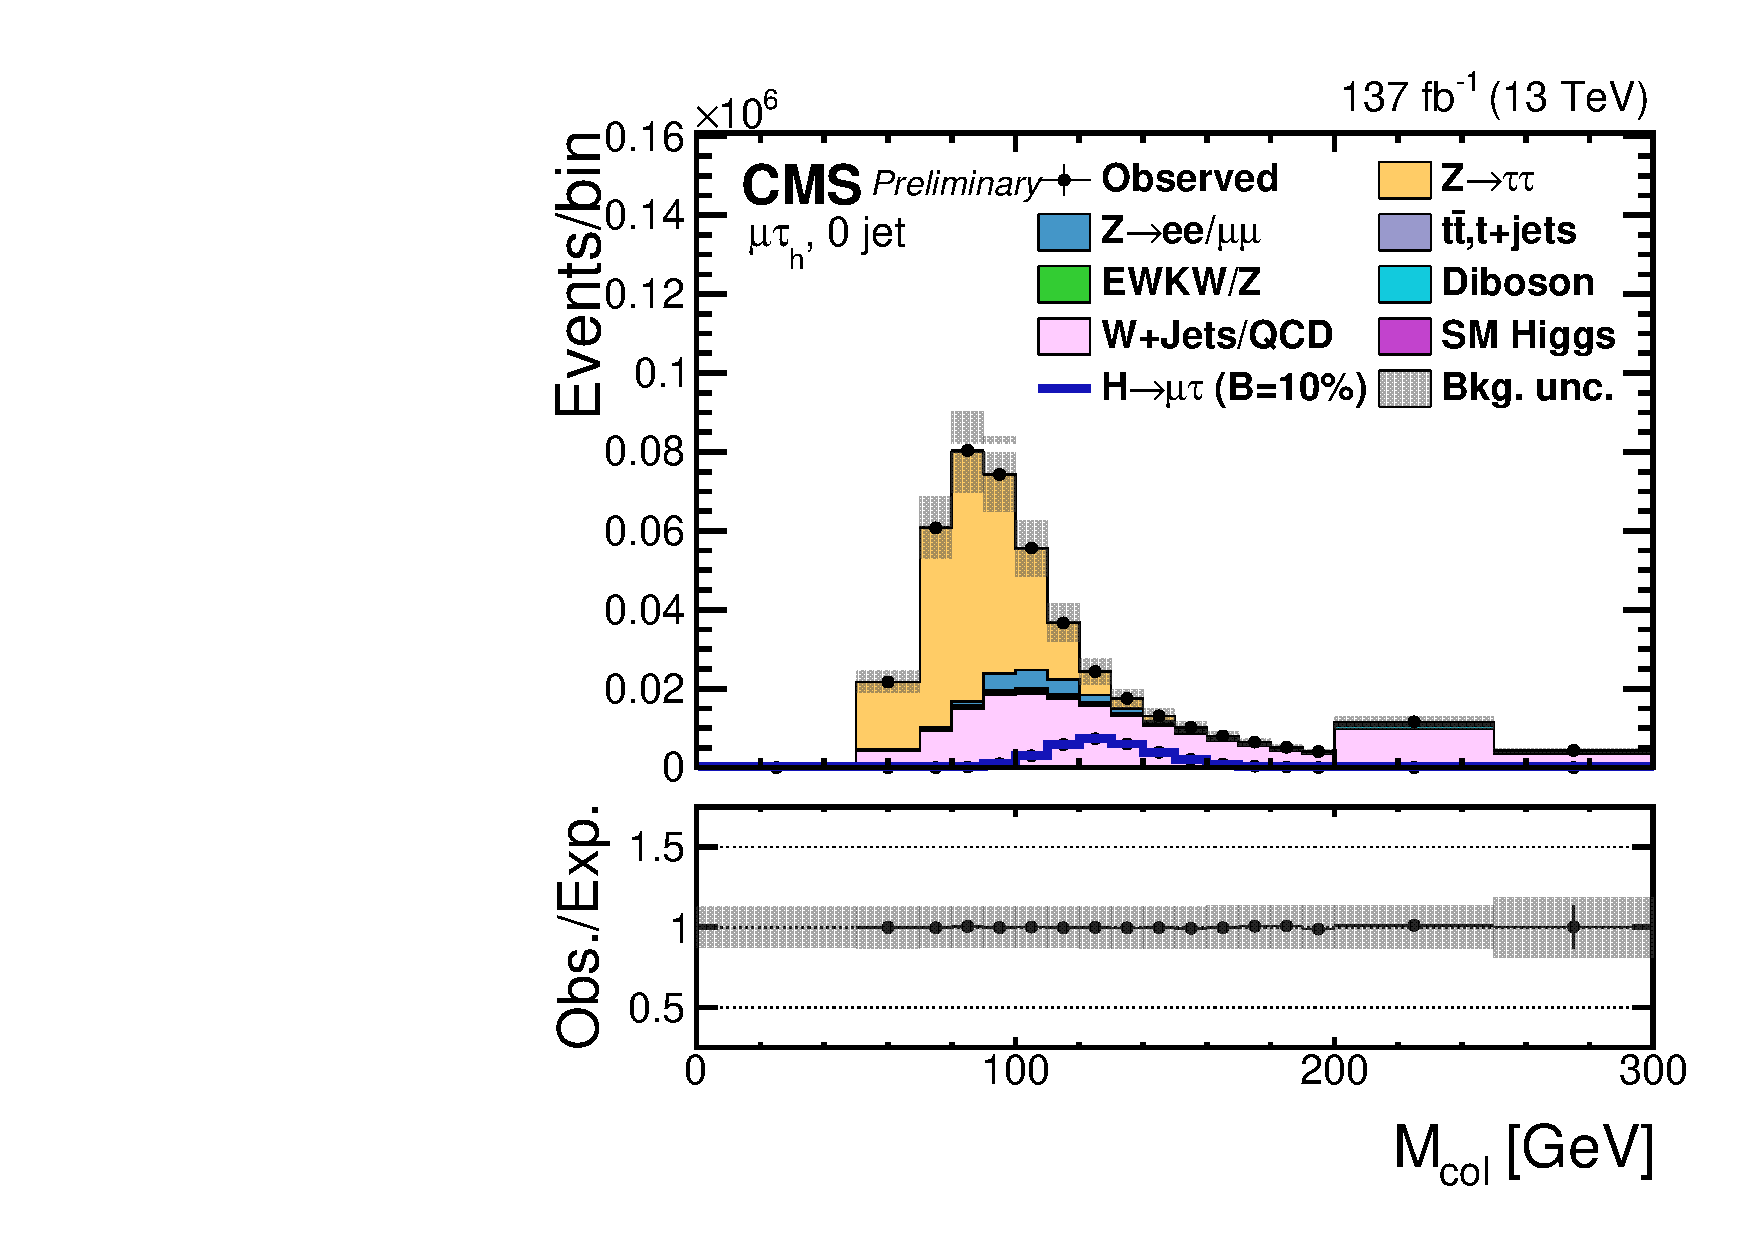
\includegraphics[width=0.4\textwidth]{plots/chapter9/CB/mutau/0jet.pdf}
  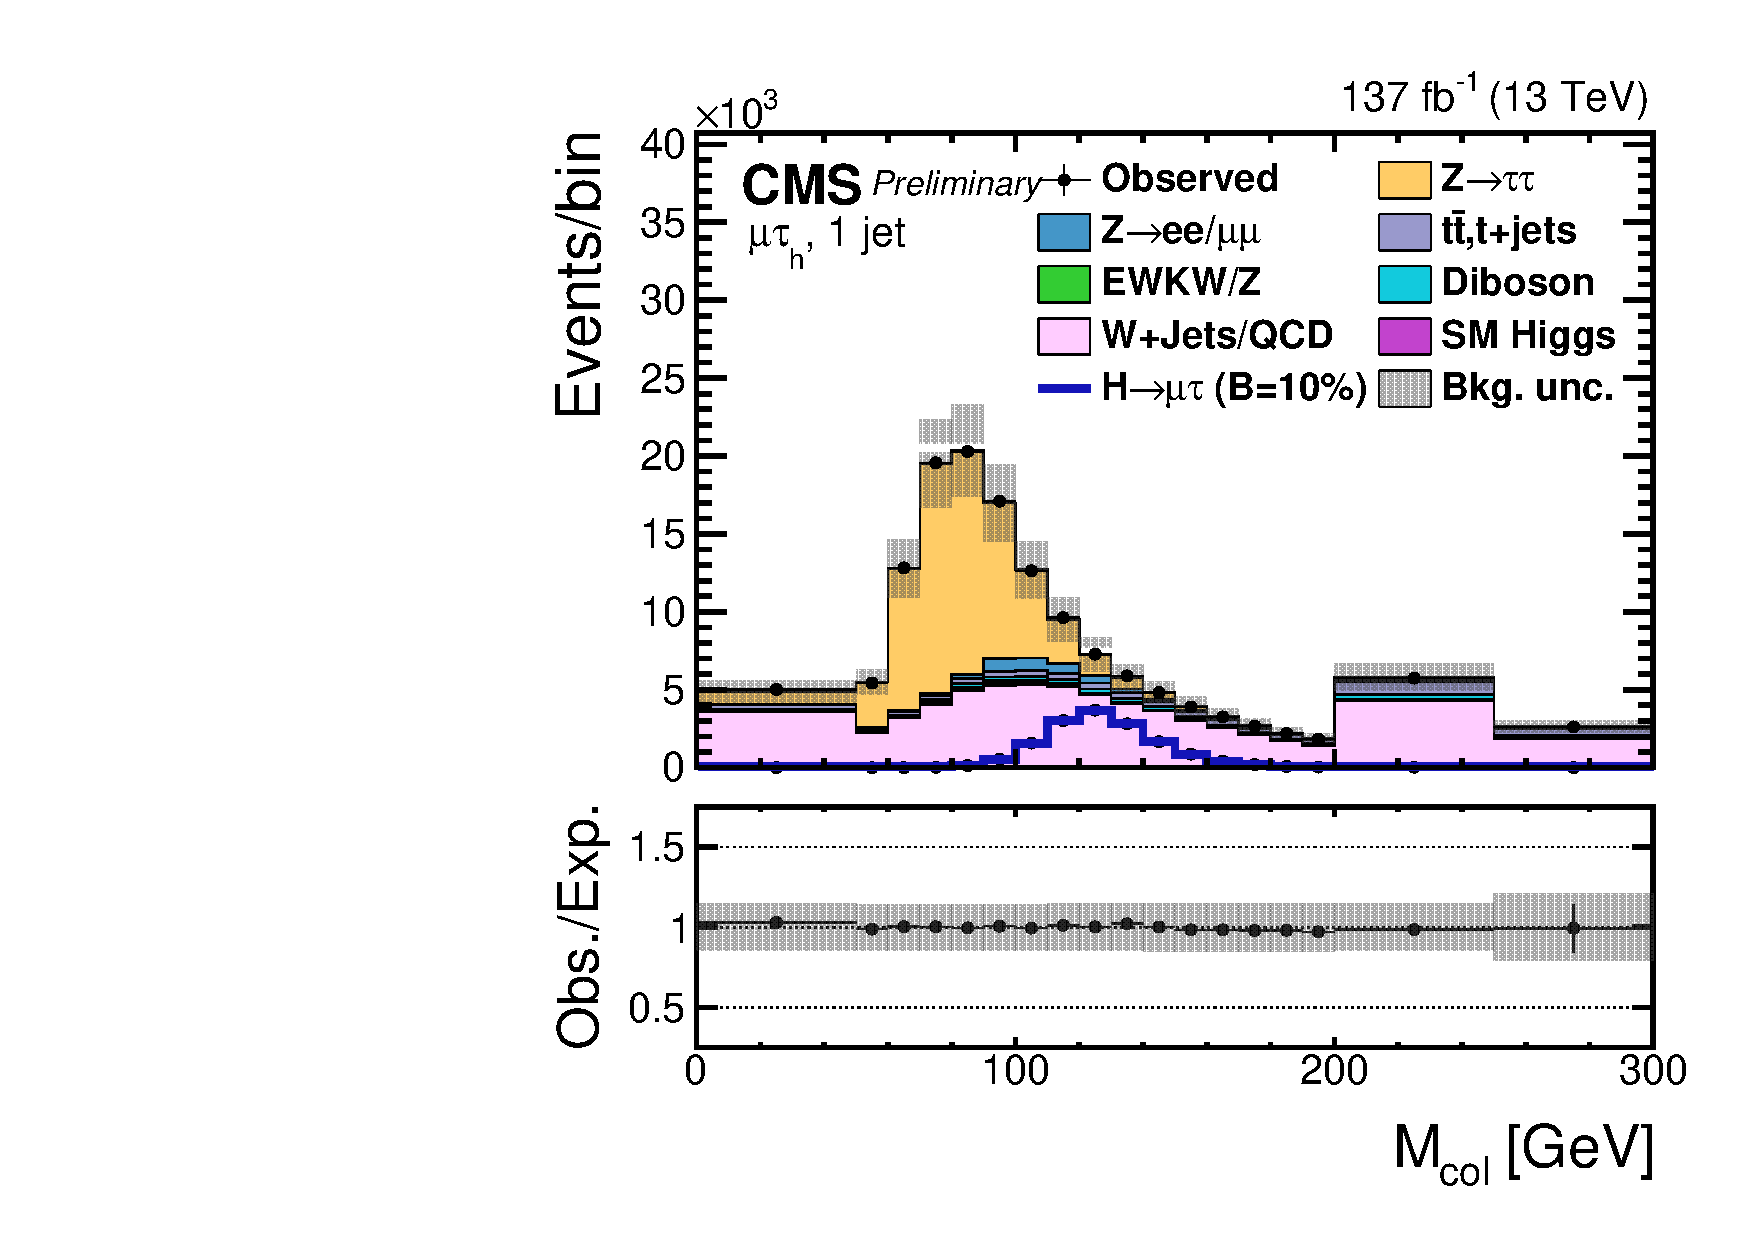
\includegraphics[width=0.4\textwidth]{plots/chapter9/CB/mutau/1jet.pdf} \\
  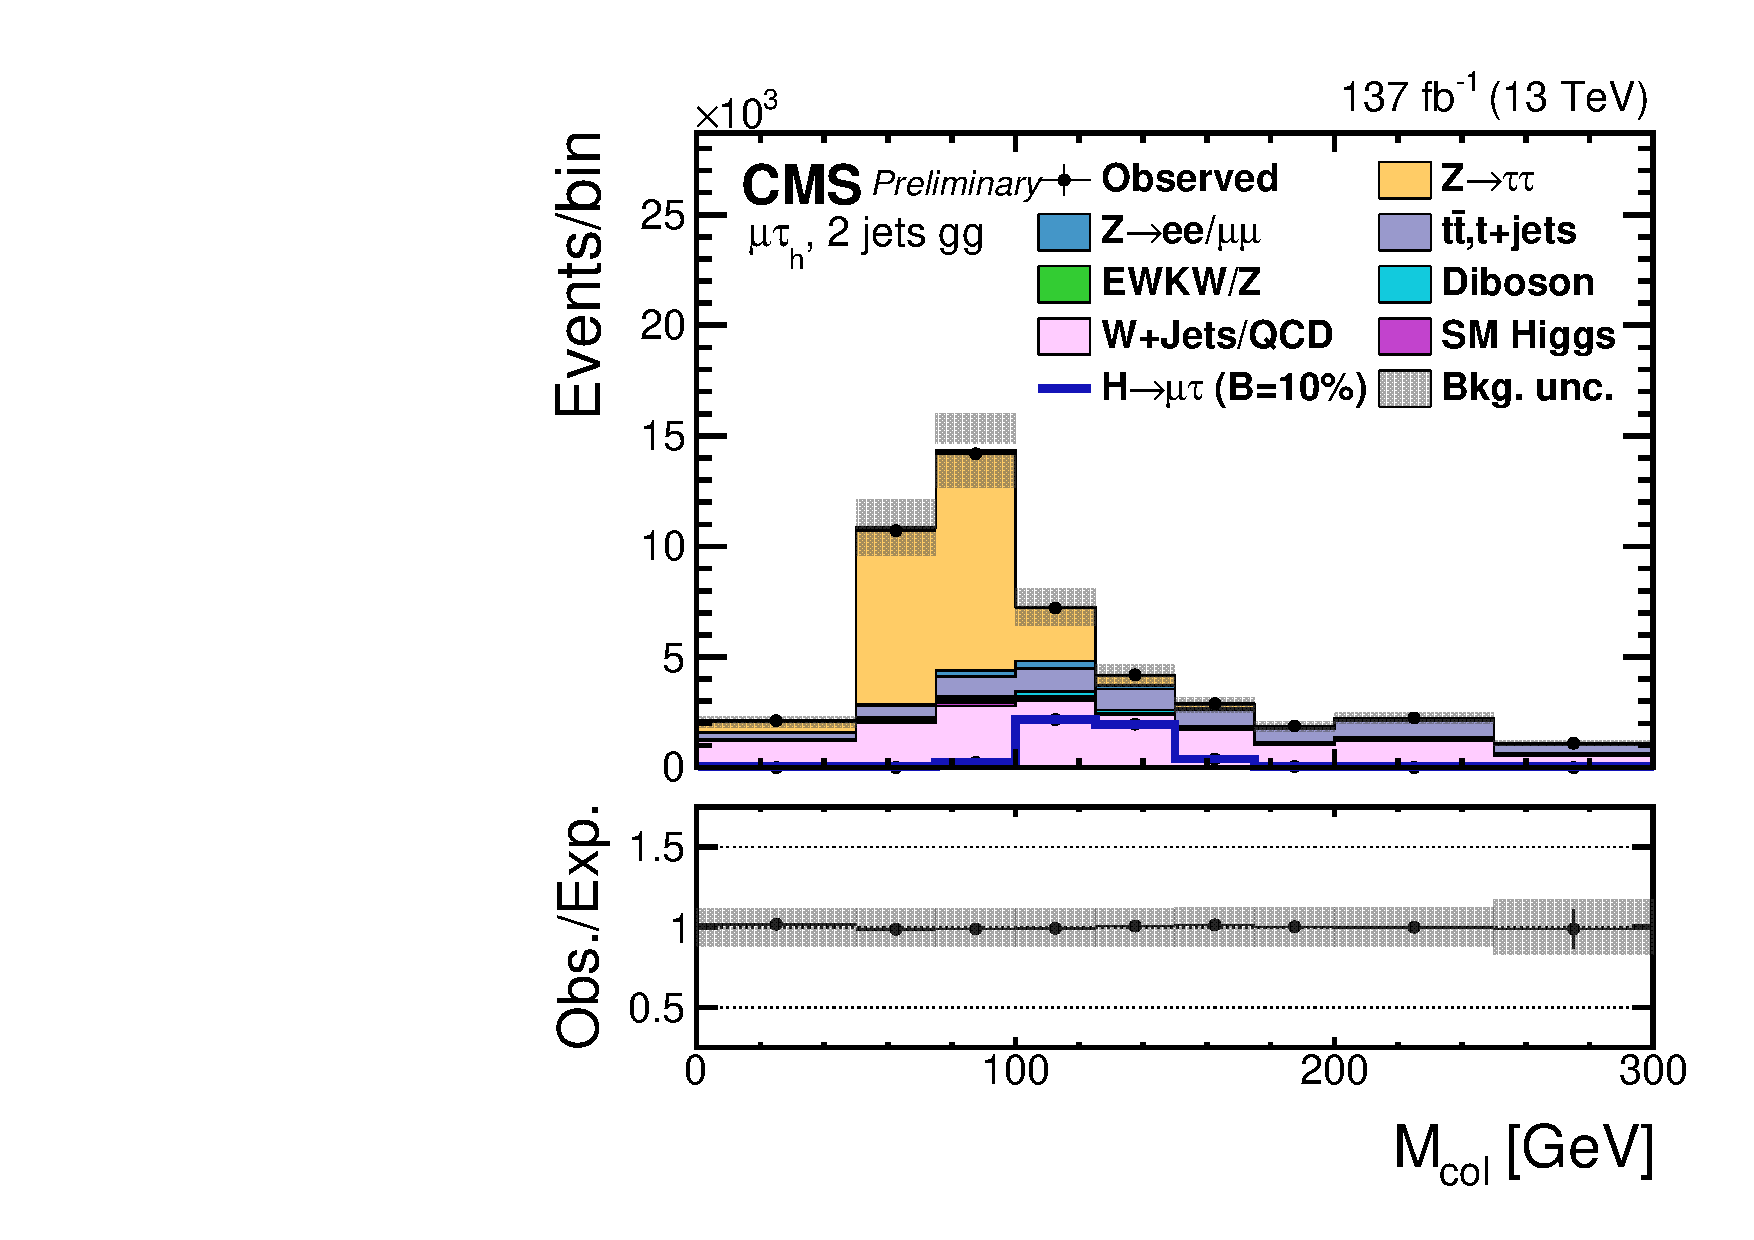
\includegraphics[width=0.4\textwidth]{plots/chapter9/CB/mutau/2jet_gg.pdf}
  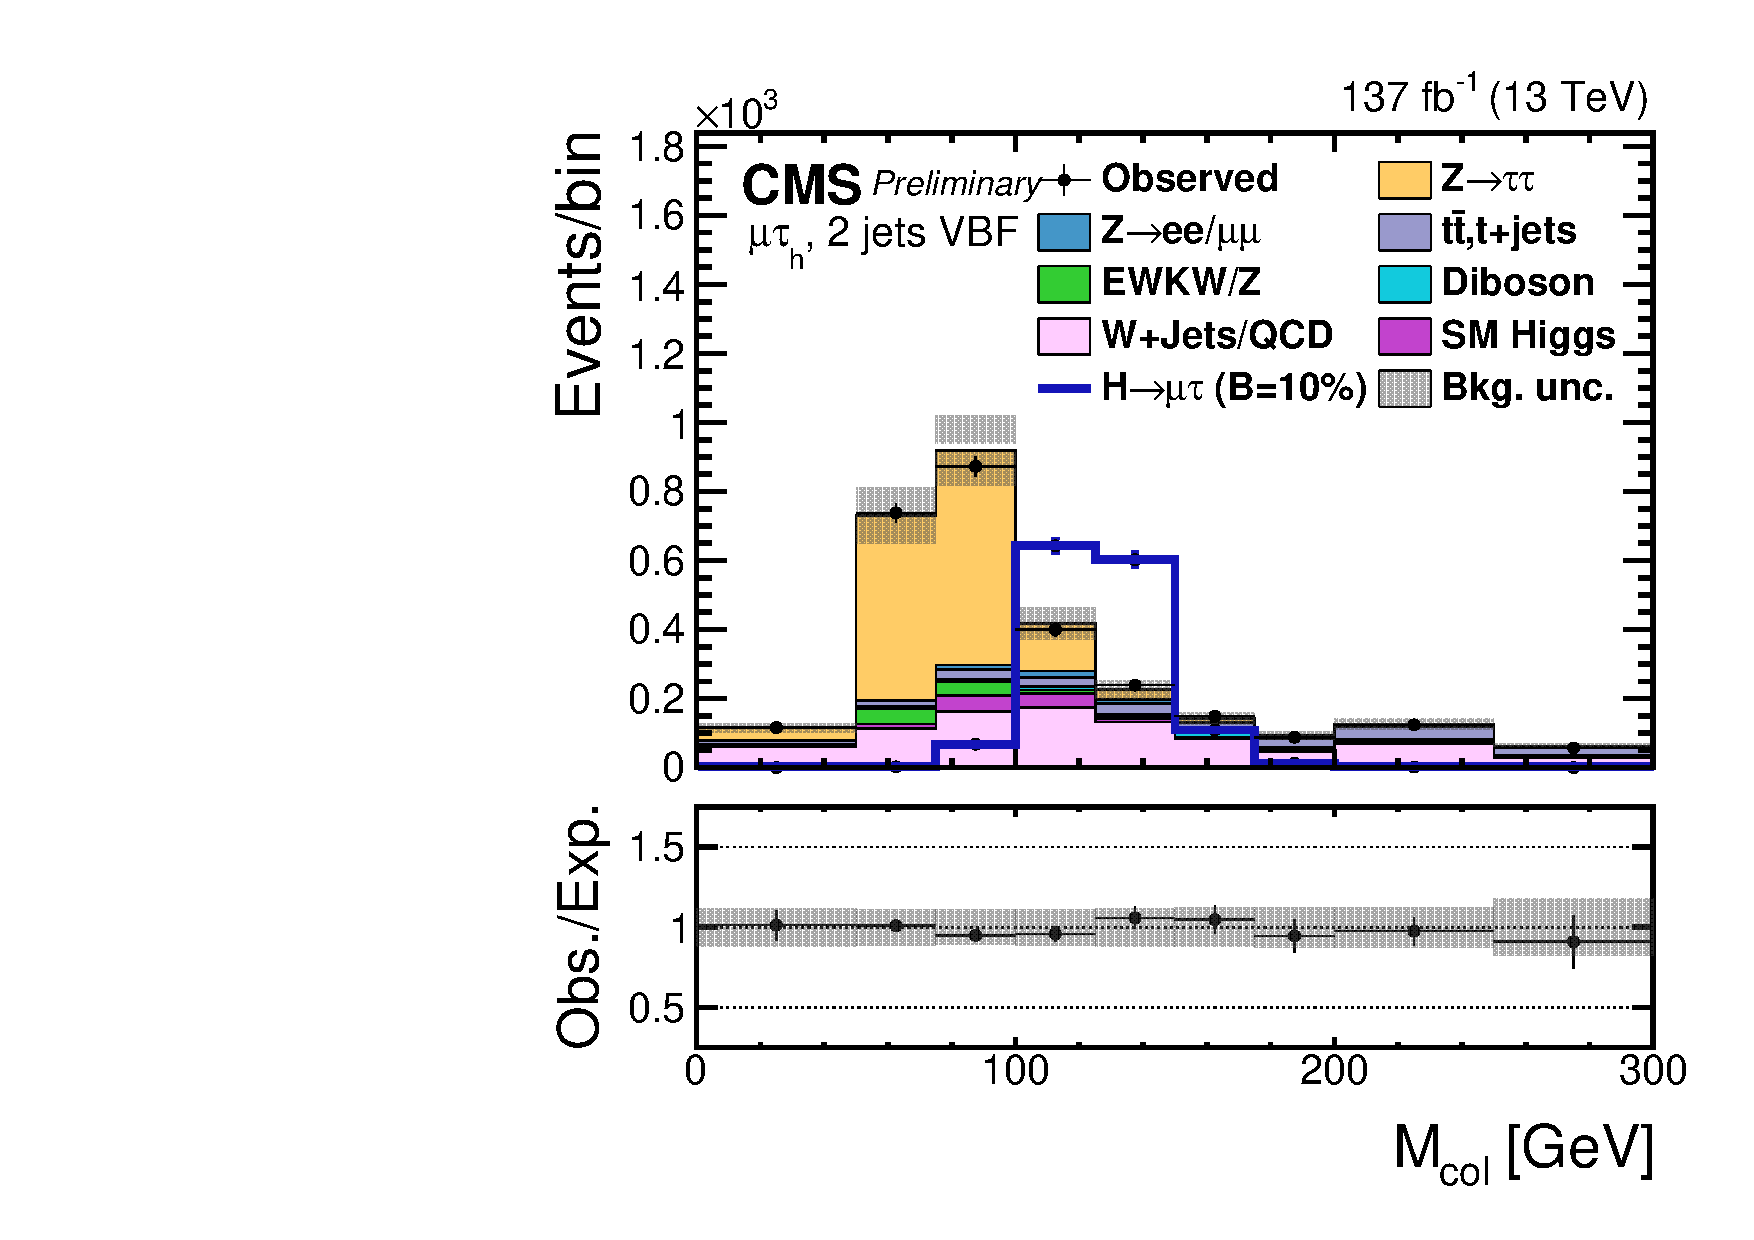
\includegraphics[width=0.4\textwidth]{plots/chapter9/CB/mutau/2jet_vbf.pdf} \\
  \caption{\mcol distributions for the observed and estimated background in the \muhad channel. The background is normalized to the best fit values from the signal plus background fit. Signal corresponds to \BHmt = 10\%. The \muhad channel categories are 0 jets (top left), 1 jet (top right), 2 jets gg (bottom left), and 2 jets VBF (bottom right). The bottom panel in each plot shows the fractional difference between the observed and estimated background. The uncertainty band shows the statistical and systematic uncertainties added in quadrature.}
  \label{fig:mcol_muhad}
\end{figure}

\begin{figure}[htbp!]
  \centering
  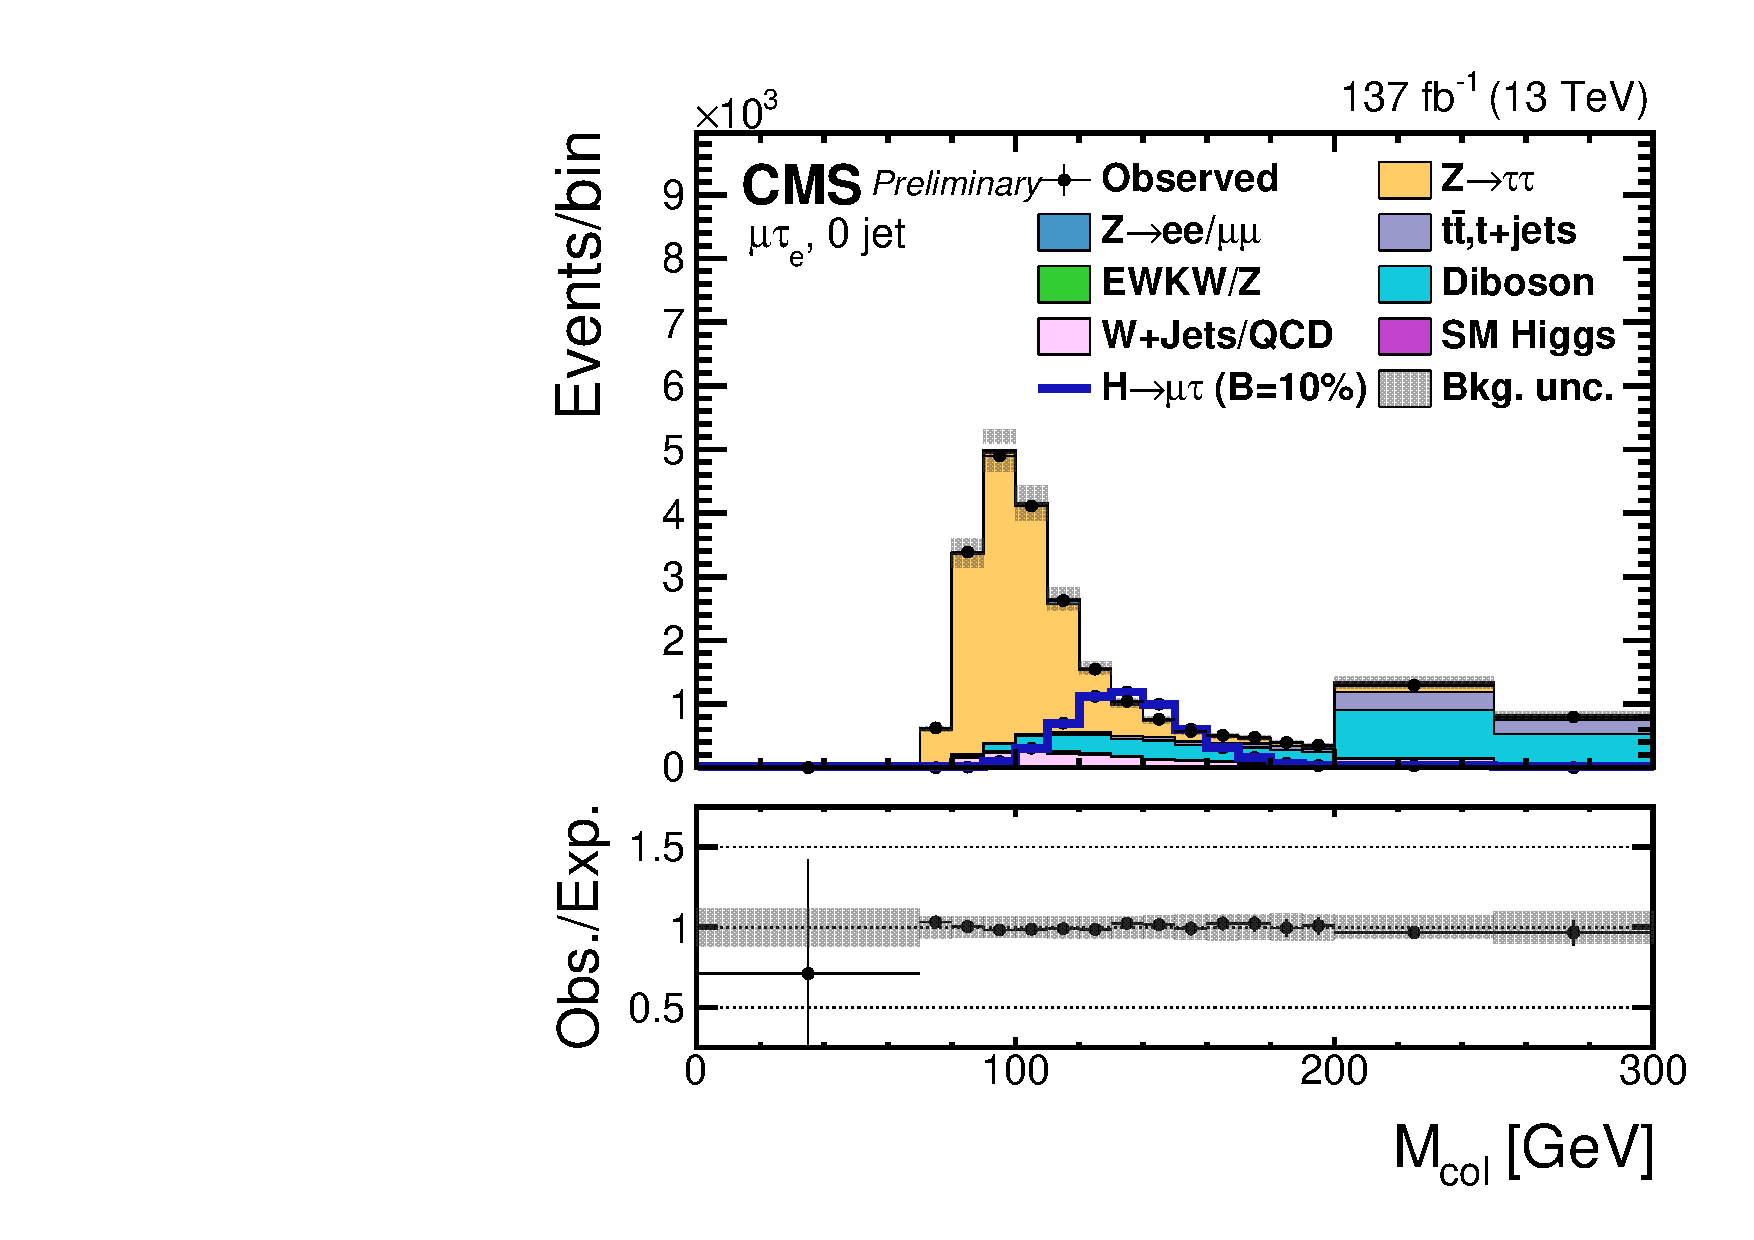
\includegraphics[width=0.4\textwidth]{plots/chapter9/CB/mue/0jet.pdf}
  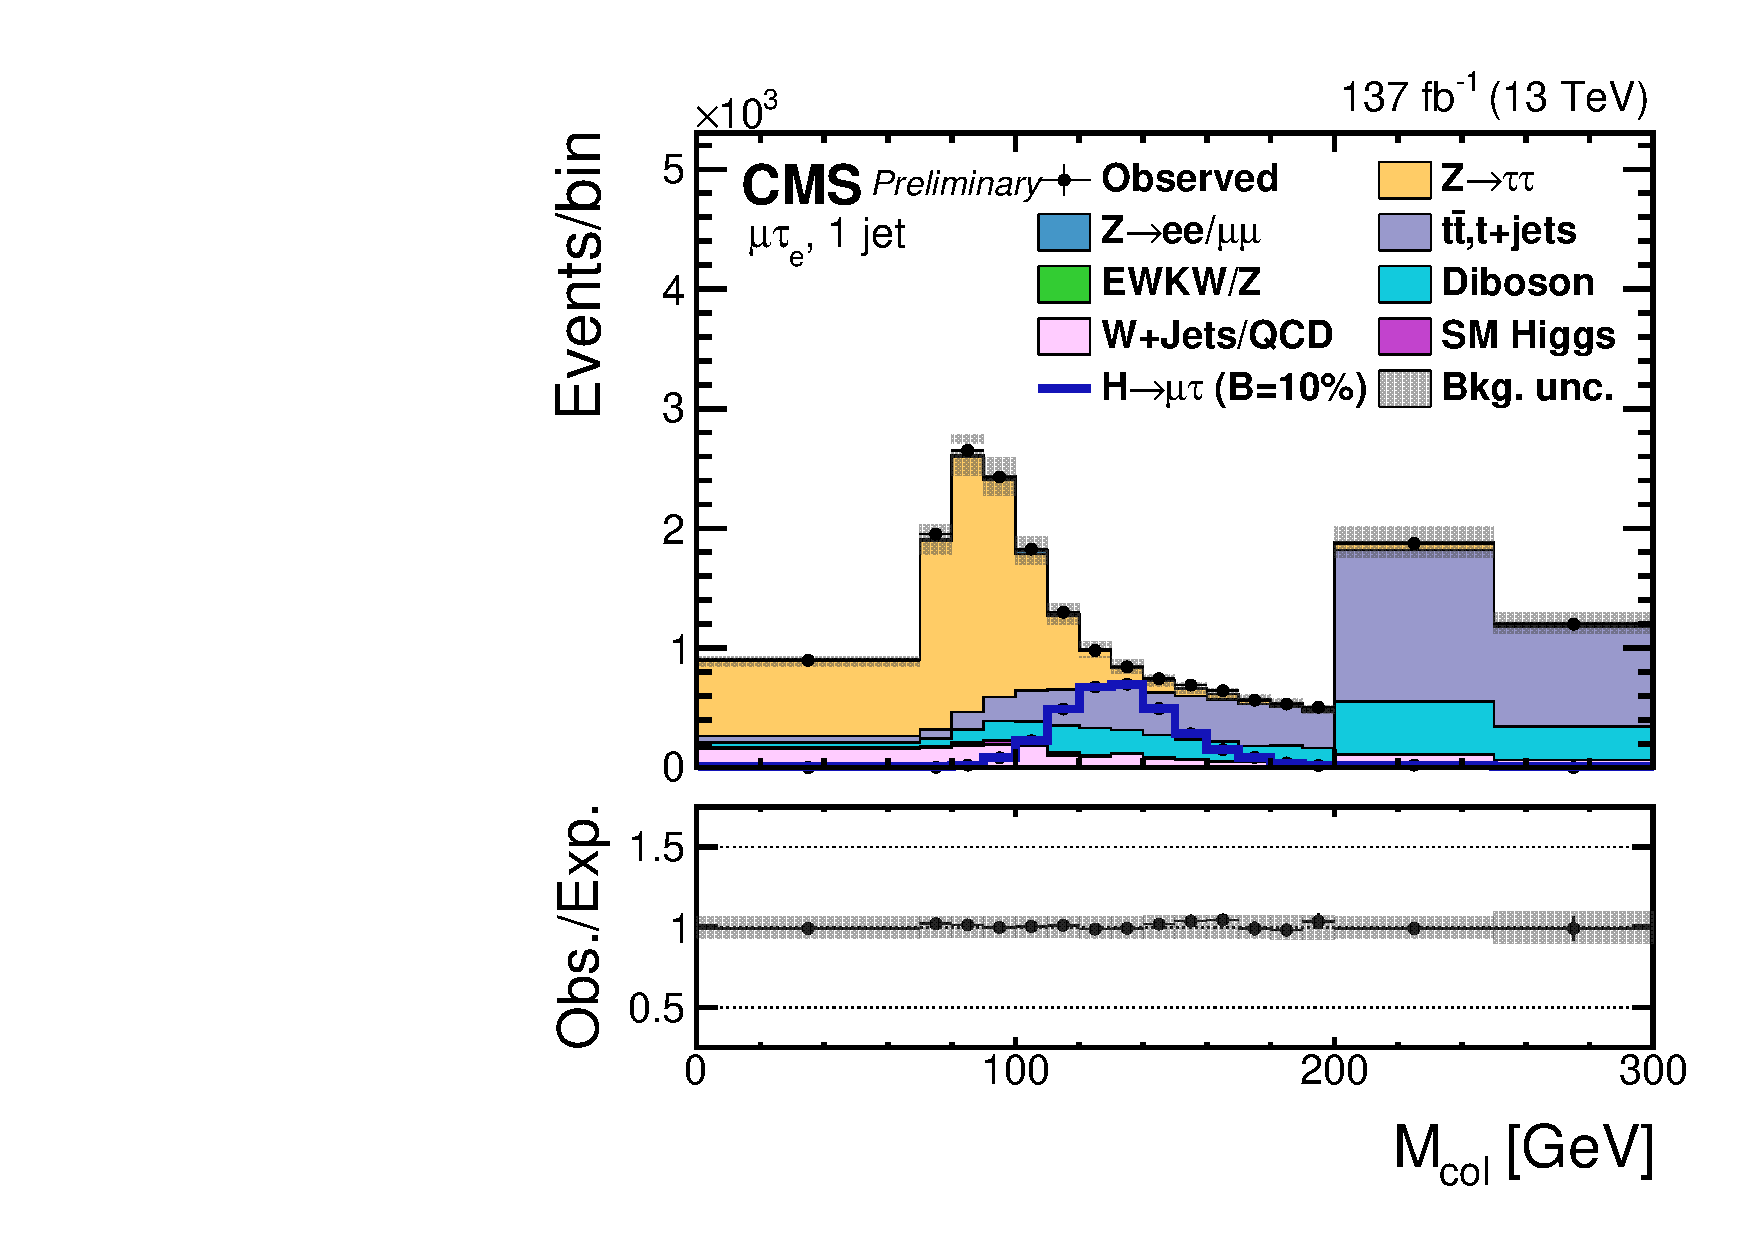
\includegraphics[width=0.4\textwidth]{plots/chapter9/CB/mue/1jet.pdf} \\
  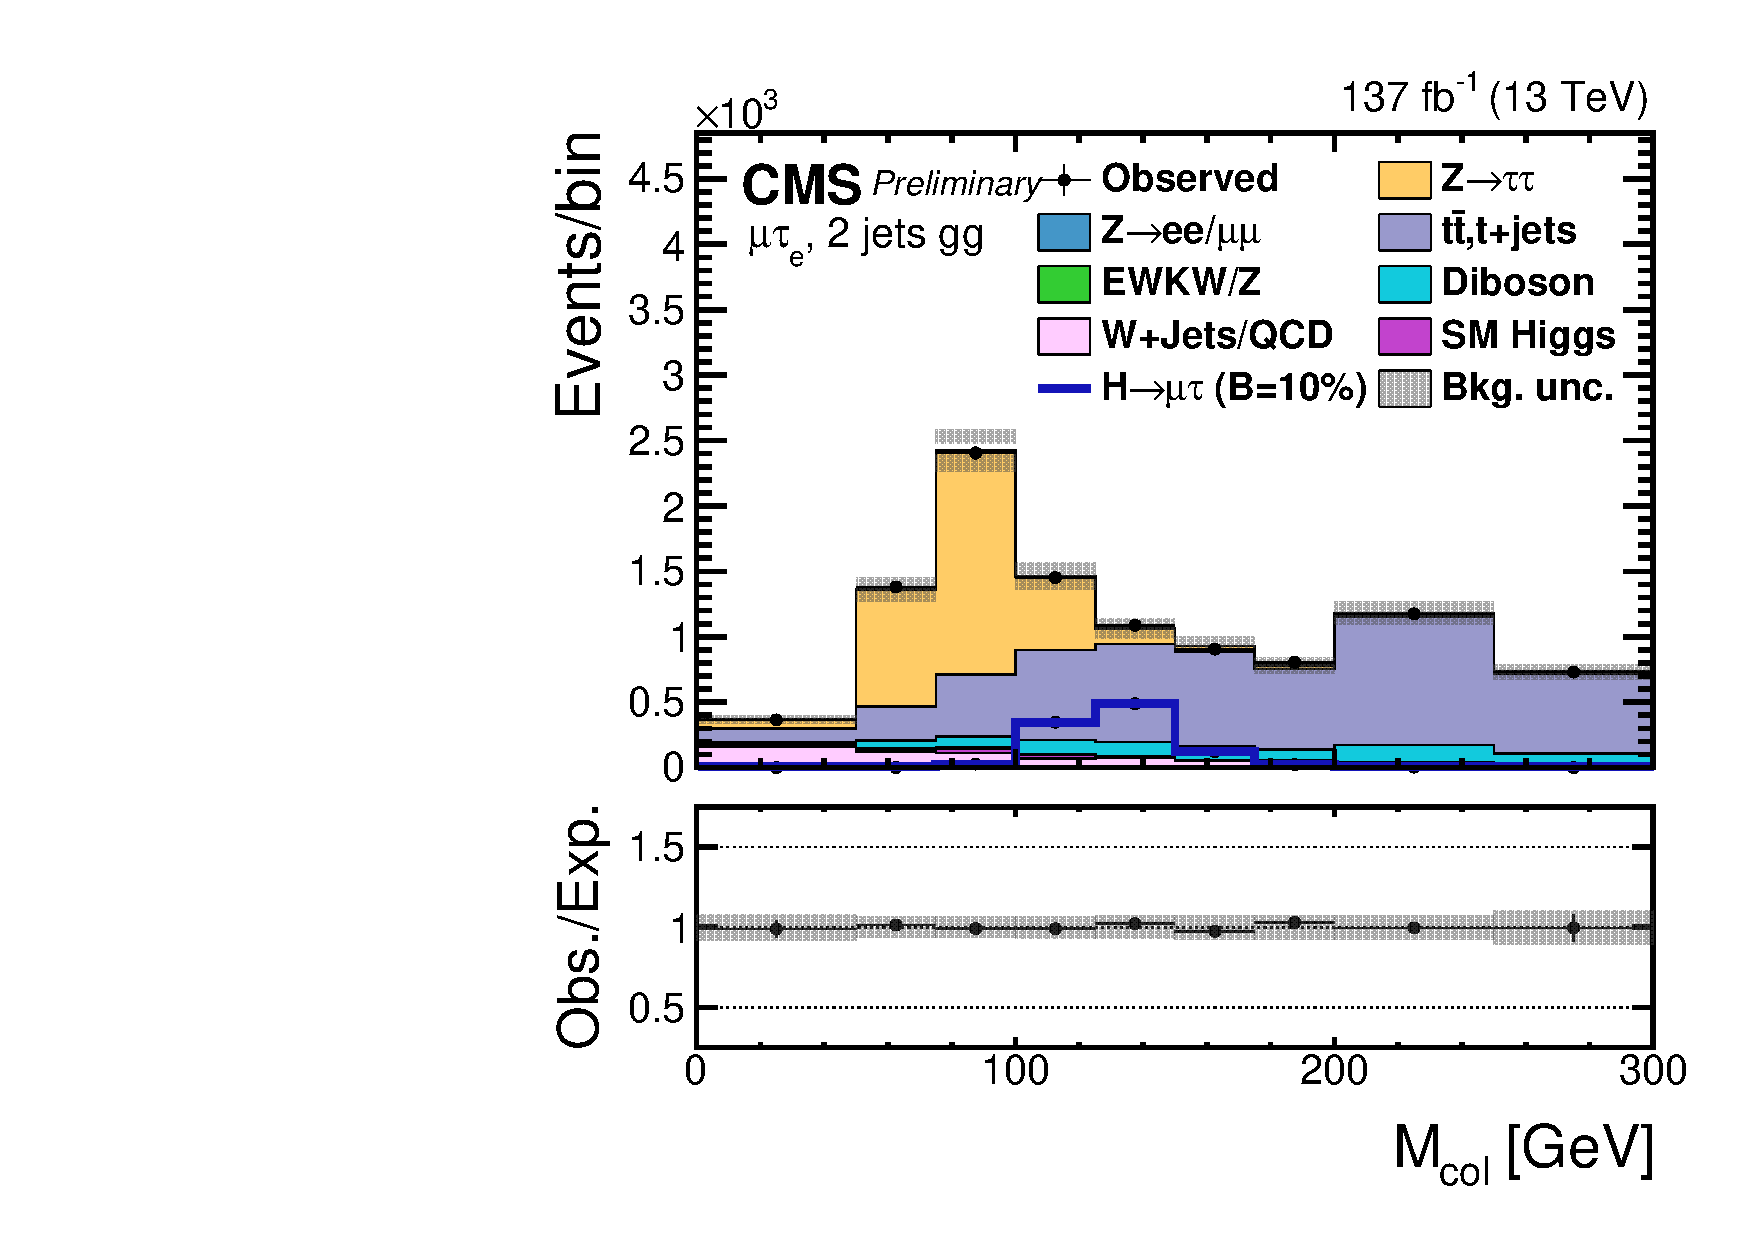
\includegraphics[width=0.4\textwidth]{plots/chapter9/CB/mue/2jet_gg.pdf}
  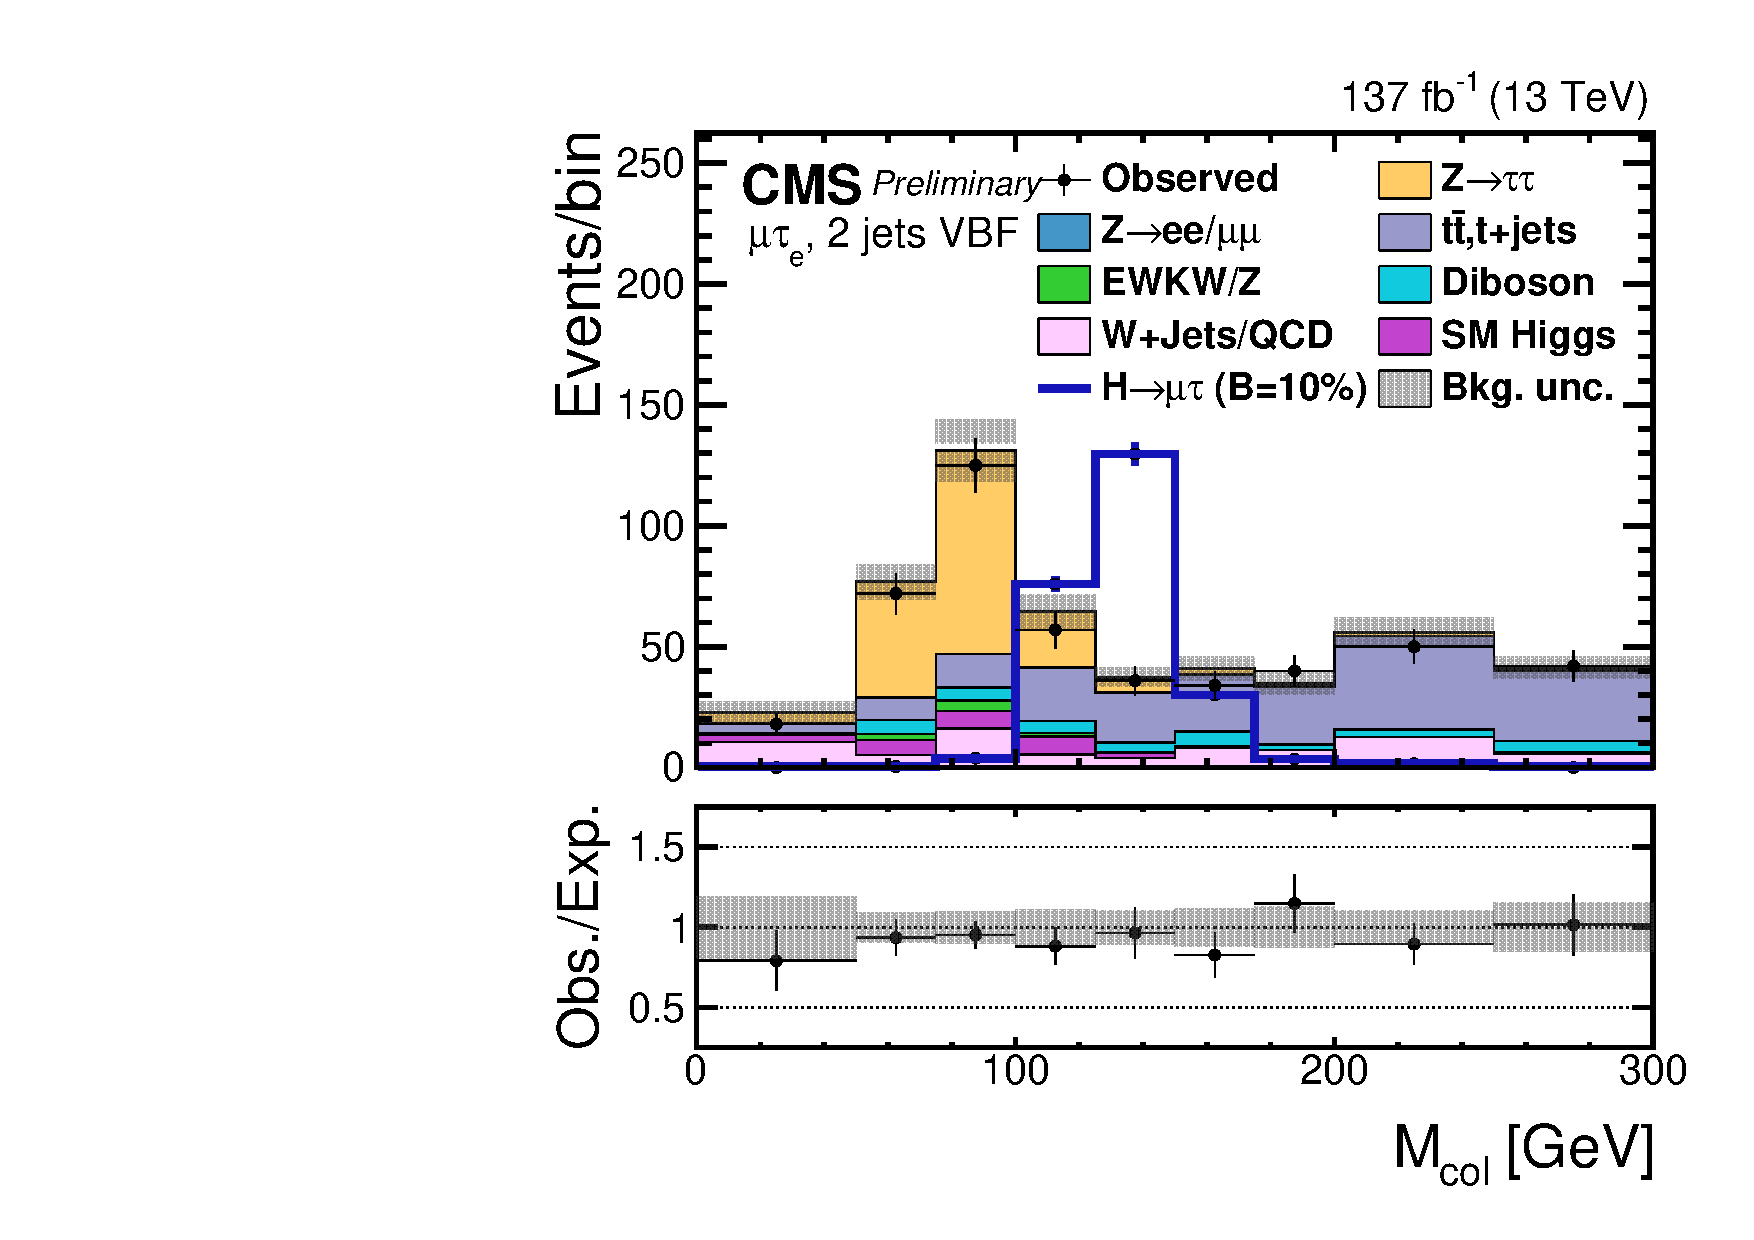
\includegraphics[width=0.4\textwidth]{plots/chapter9/CB/mue/2jet_vbf.pdf} \\
  \caption{\mcol distributions for the observed and estimated background in the \mue channel. The background is normalized to the best fit values from the signal plus background fit. Signal corresponds to \BHmt = 10\%. The \mue channel categories are 0 jets (top left), 1 jet (top right), 2 jets gg (bottom left), and 2 jets VBF (bottom right). The bottom panel in each plot shows the fractional difference between the observed and estimated background. The uncertainty band shows the statistical and systematic uncertainties added in quadrature.}
  \label{fig:mcol_mue}
\end{figure}

\begin{figure}[htbp!]
  \centering
  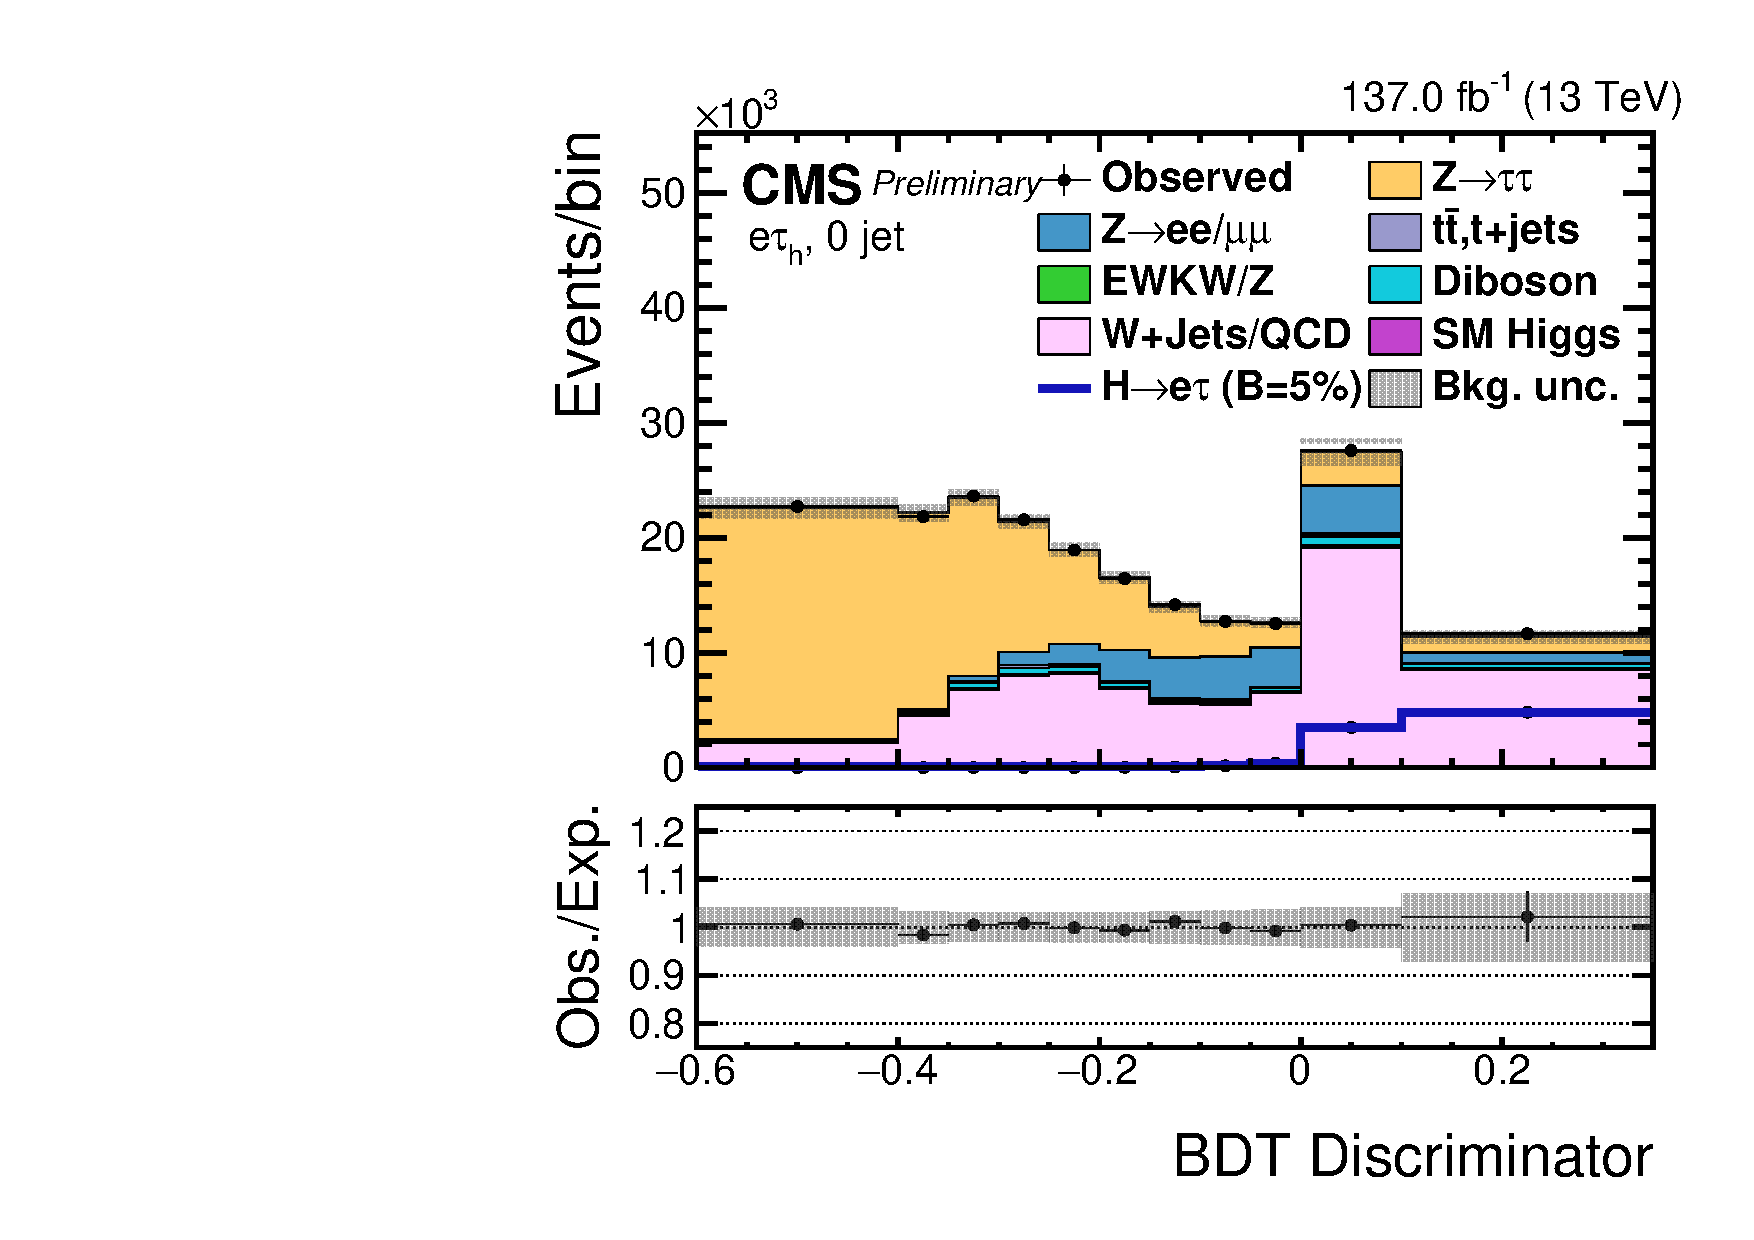
\includegraphics[width=0.4\textwidth]{plots/chapter9/BDT/etau/0jet.pdf}
  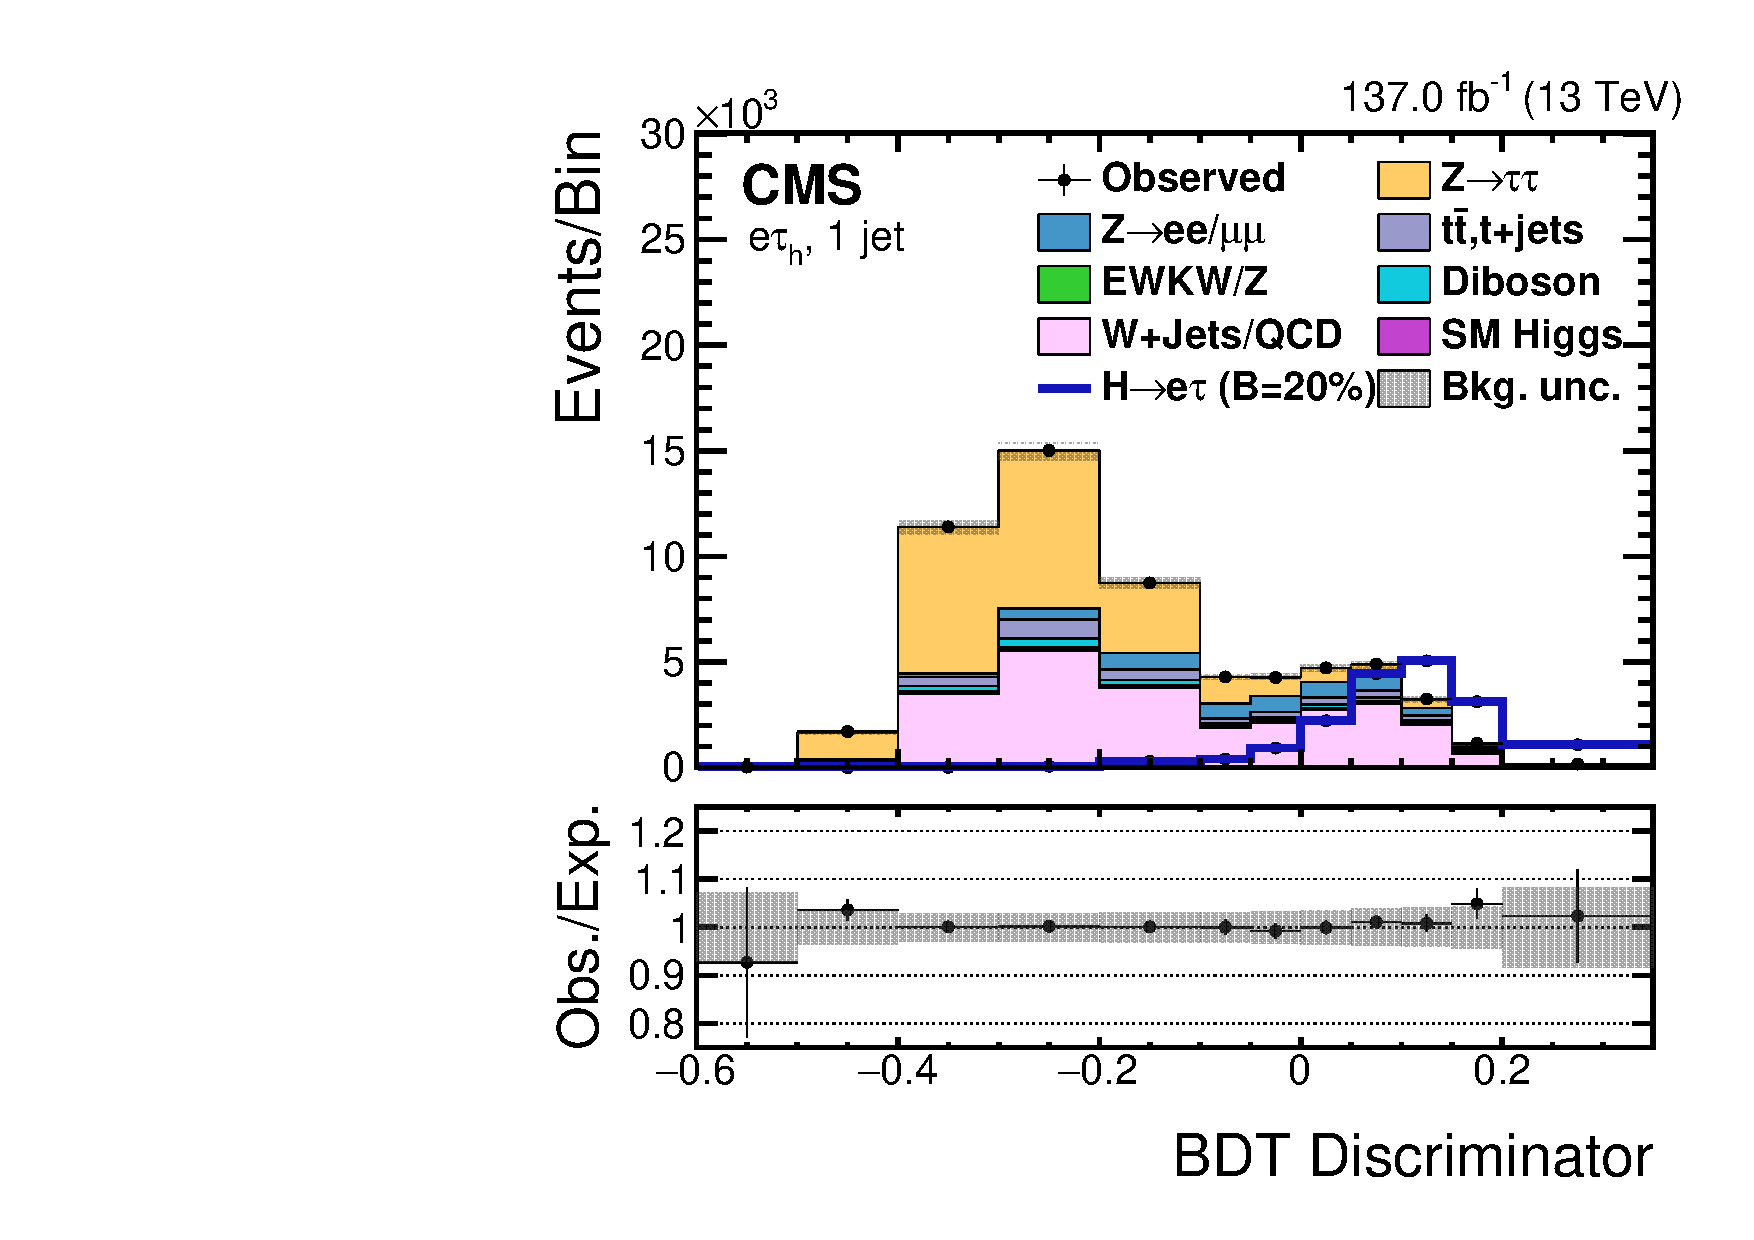
\includegraphics[width=0.4\textwidth]{plots/chapter9/BDT/etau/1jet.pdf} \\
  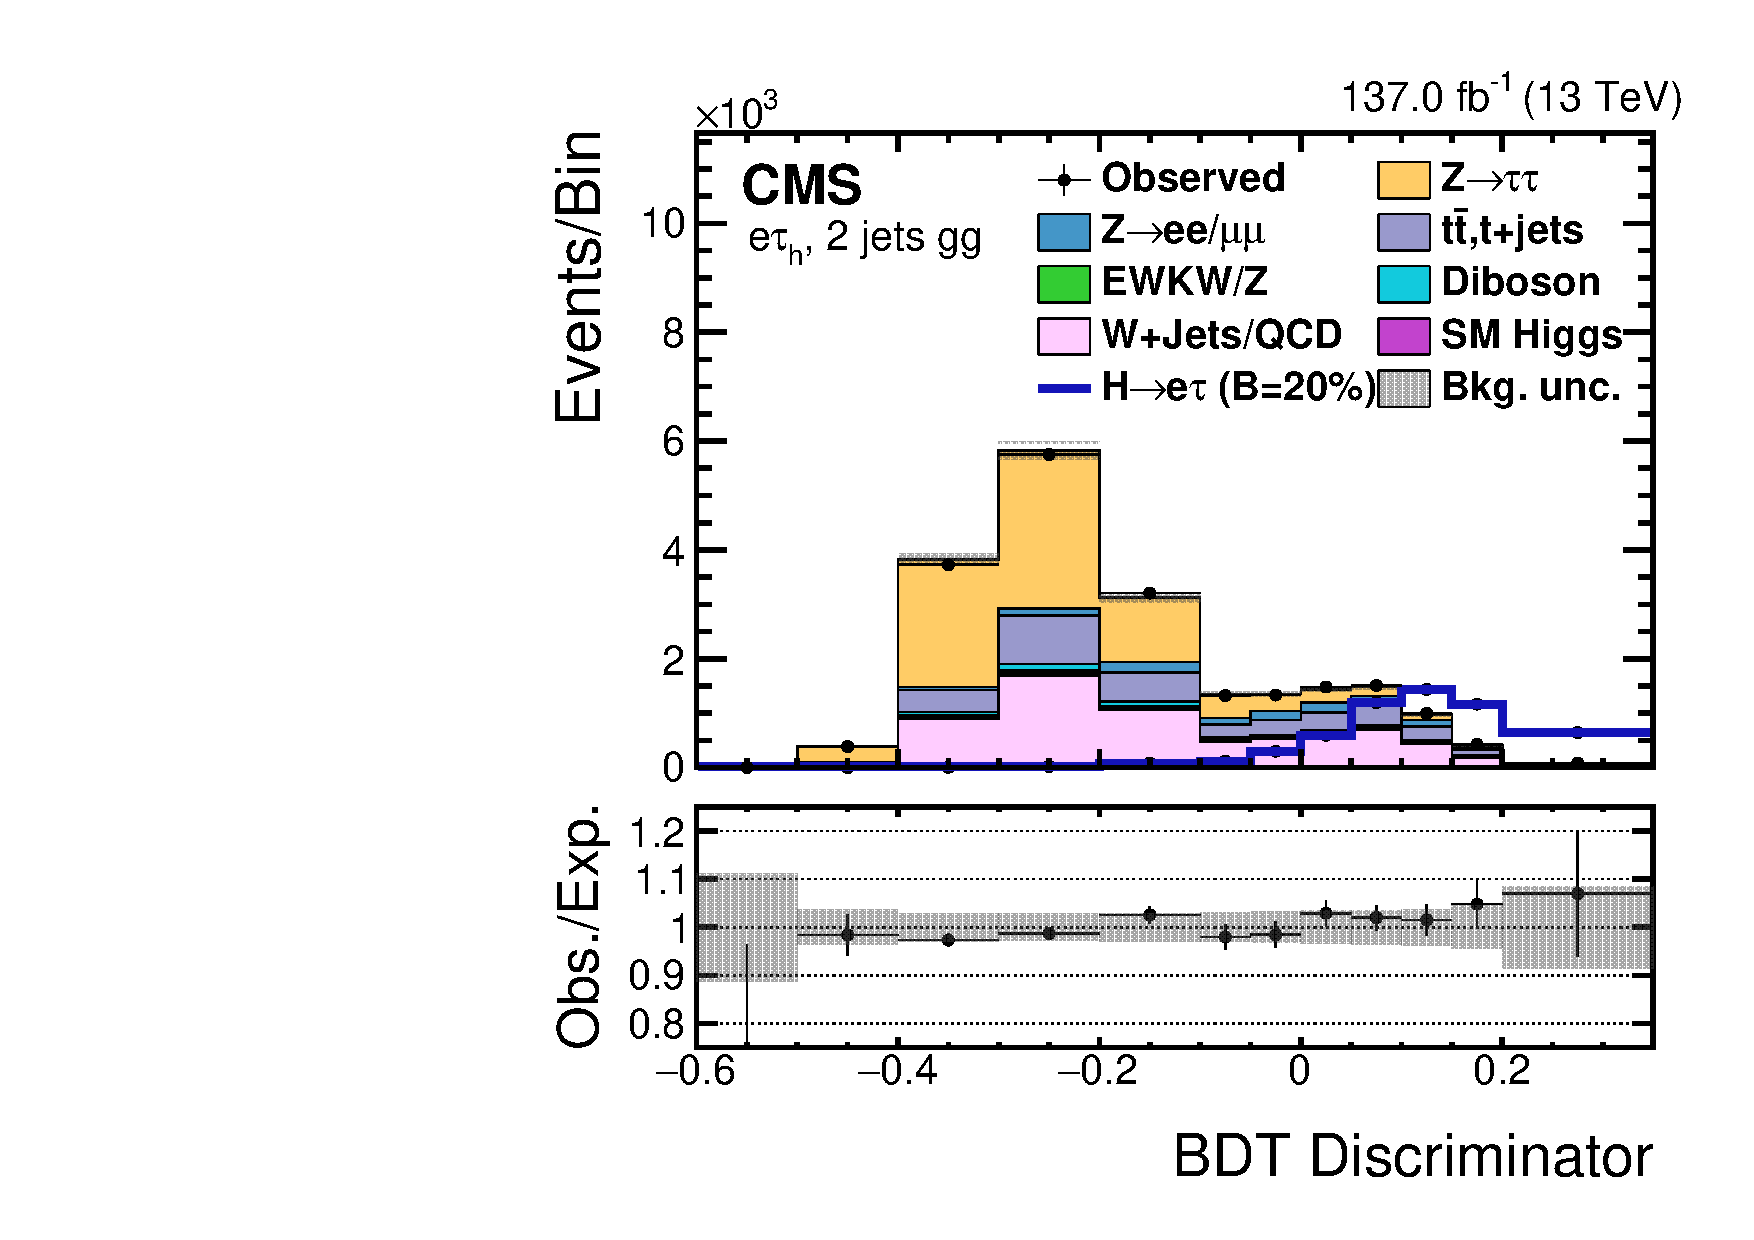
\includegraphics[width=0.4\textwidth]{plots/chapter9/BDT/etau/2jet_gg.pdf}
  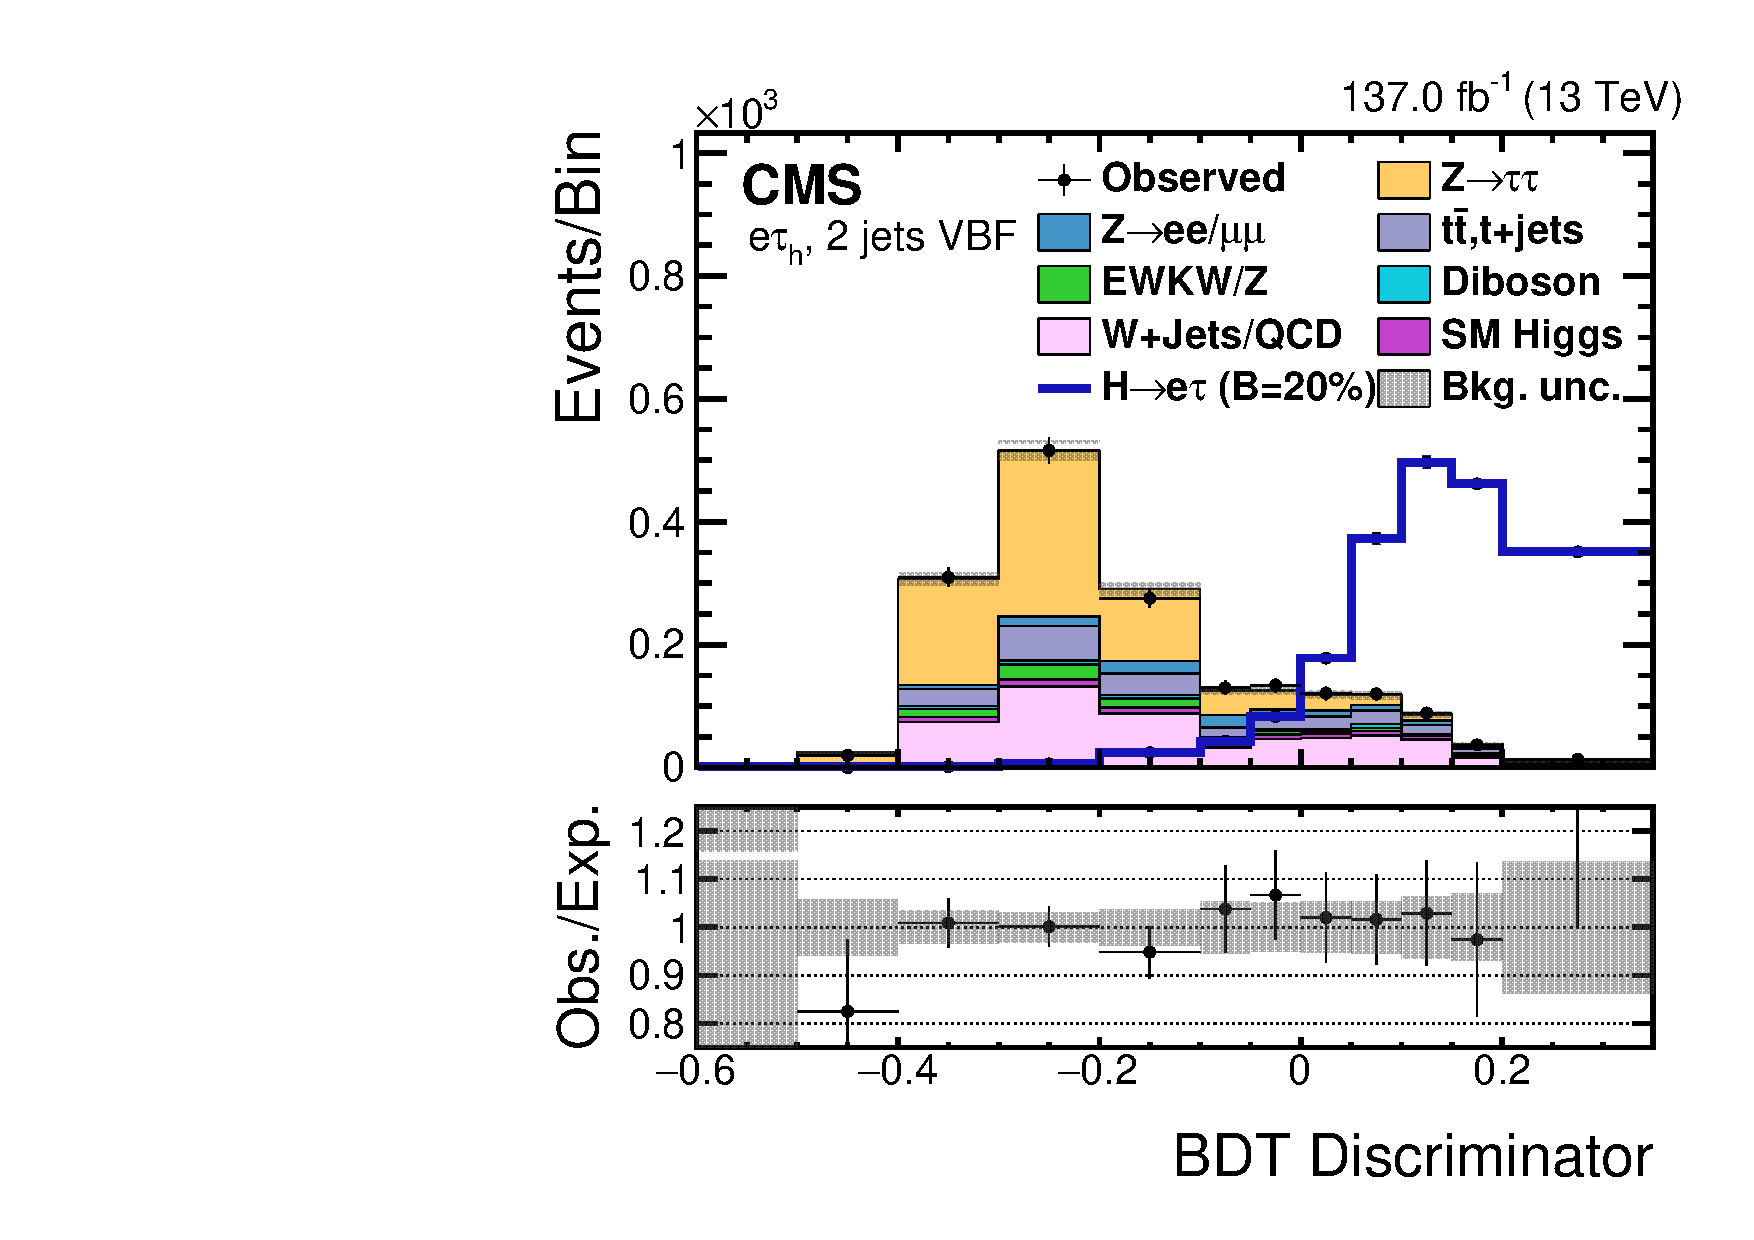
\includegraphics[width=0.4\textwidth]{plots/chapter9/BDT/etau/2jet_vbf.pdf} \\
  \caption{BDT discriminator distributions for the observed and estimated background in the \ehad channel. The background is normalized to the best fit values from the signal plus background fit. Signal corresponds to \BHet = 20\%. The \ehad channel categories are 0 jets (top left), 1 jet (top right), 2 jets gg (bottom left), and 2 jets VBF (bottom right). The bottom panel in each plot shows the fractional difference between the observed and estimated background. The uncertainty band shows the statistical and systematic uncertainties added in quadrature.}
  \label{fig:bdt_ehad}
\end{figure}

\begin{figure}[htbp!]
  \centering
  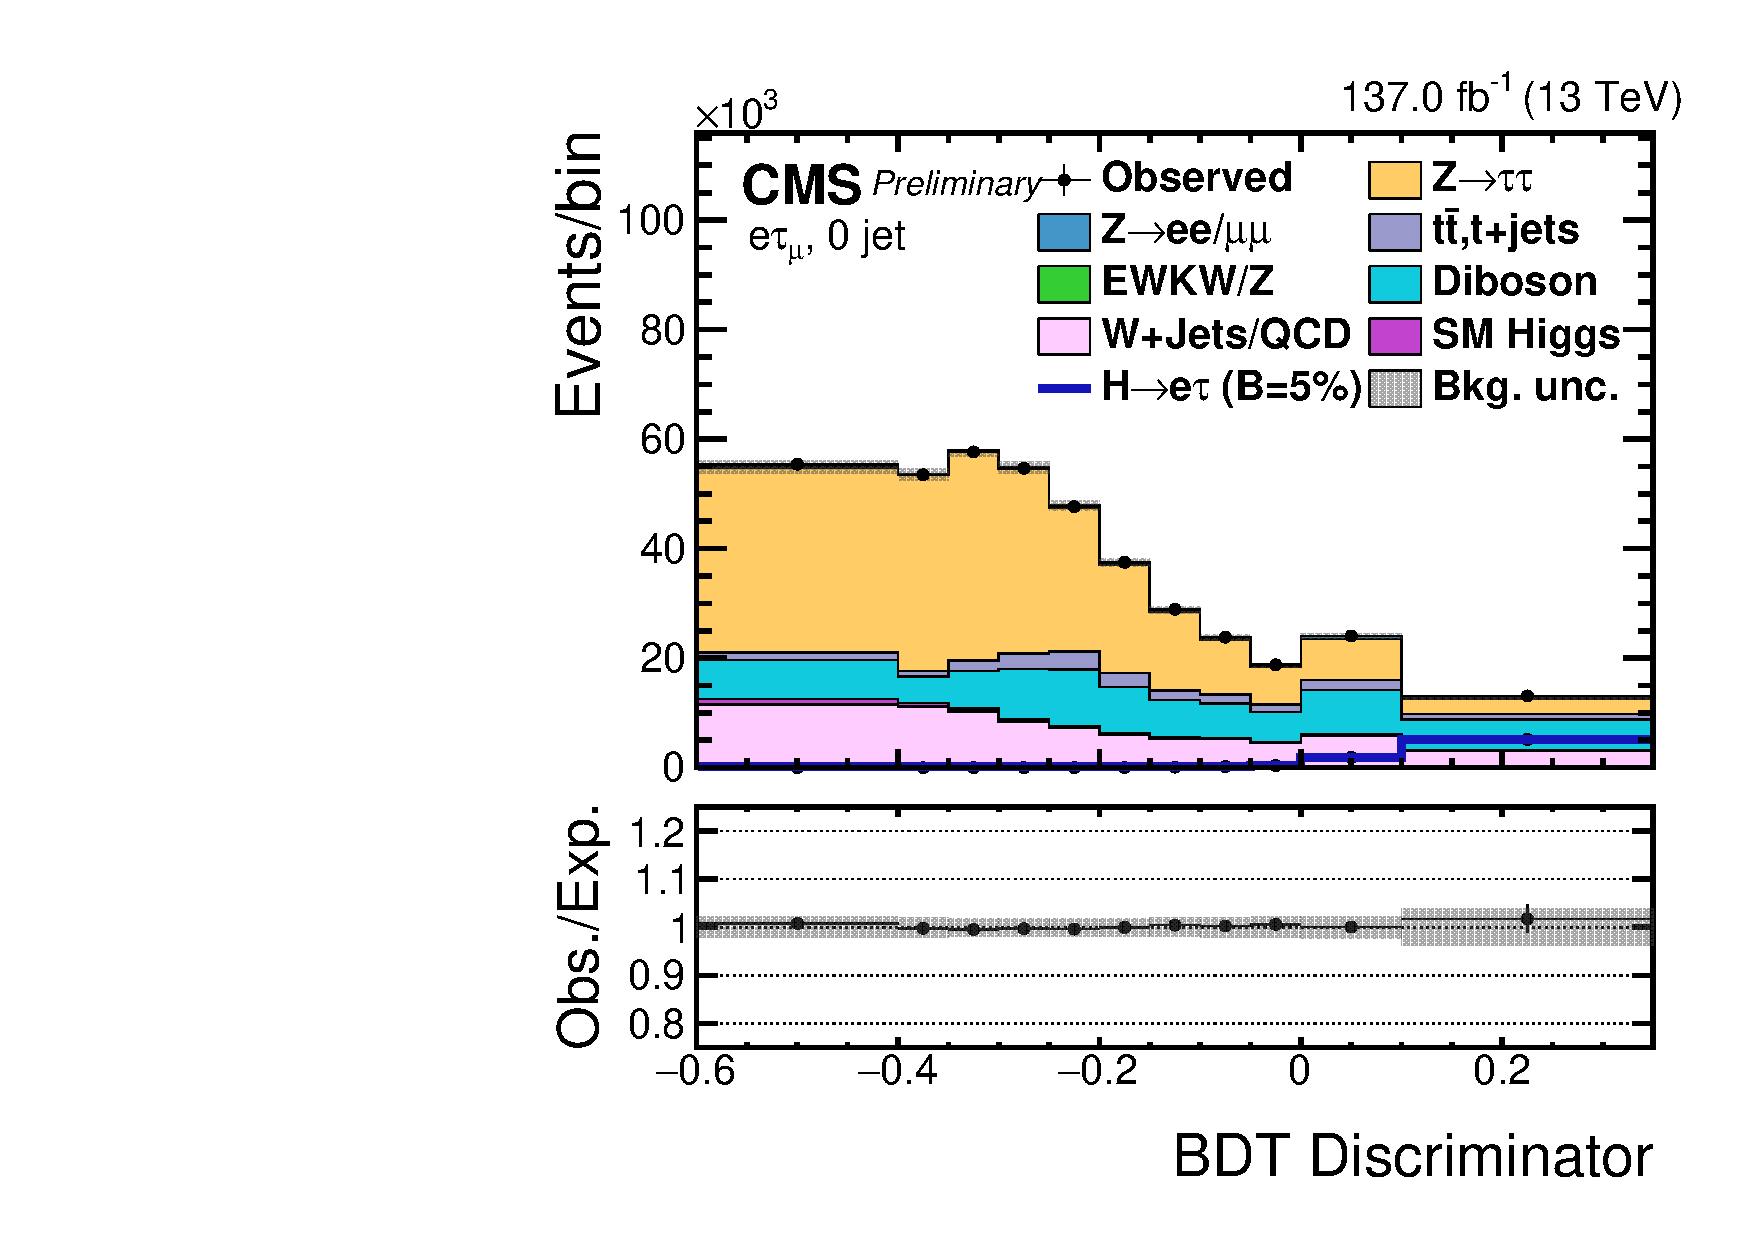
\includegraphics[width=0.4\textwidth]{plots/chapter9/BDT/emu/0jet.pdf}
  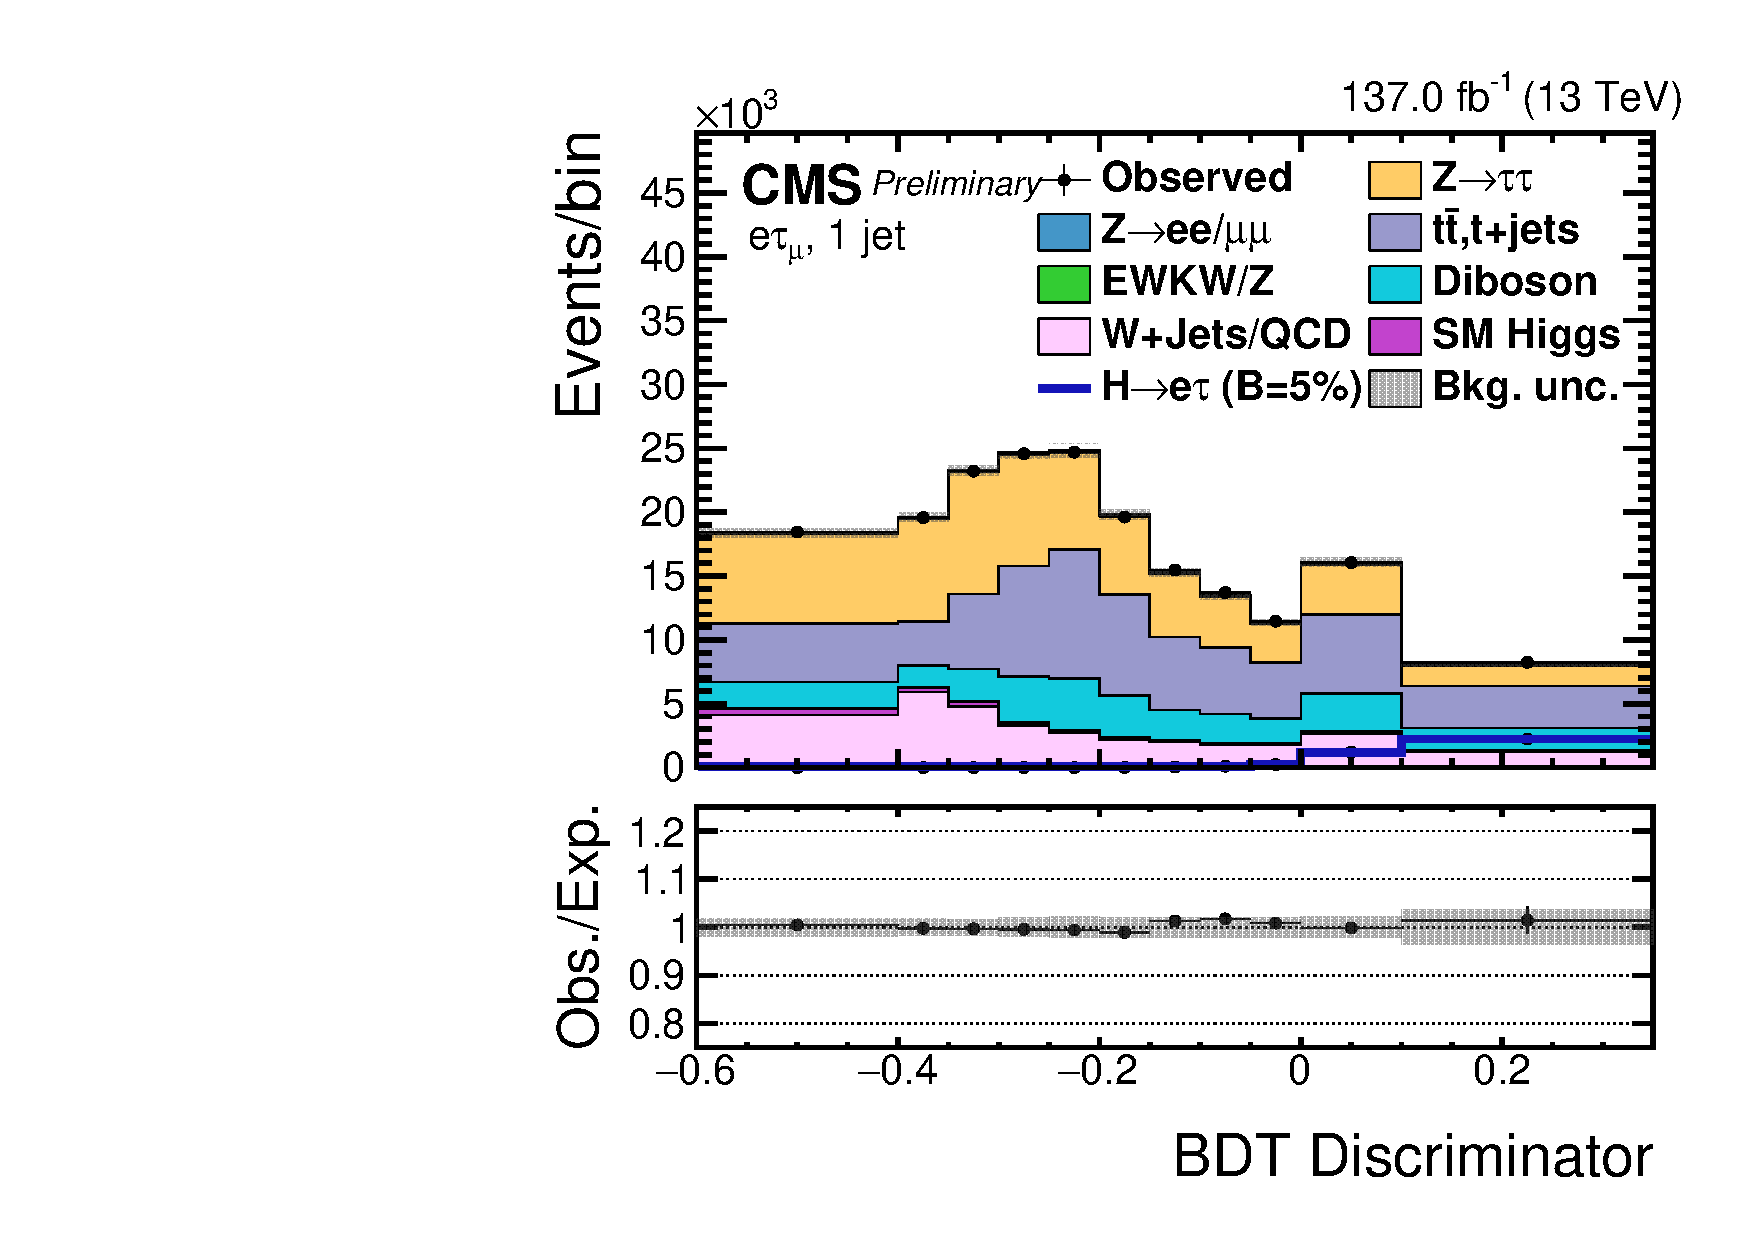
\includegraphics[width=0.4\textwidth]{plots/chapter9/BDT/emu/1jet.pdf} \\
  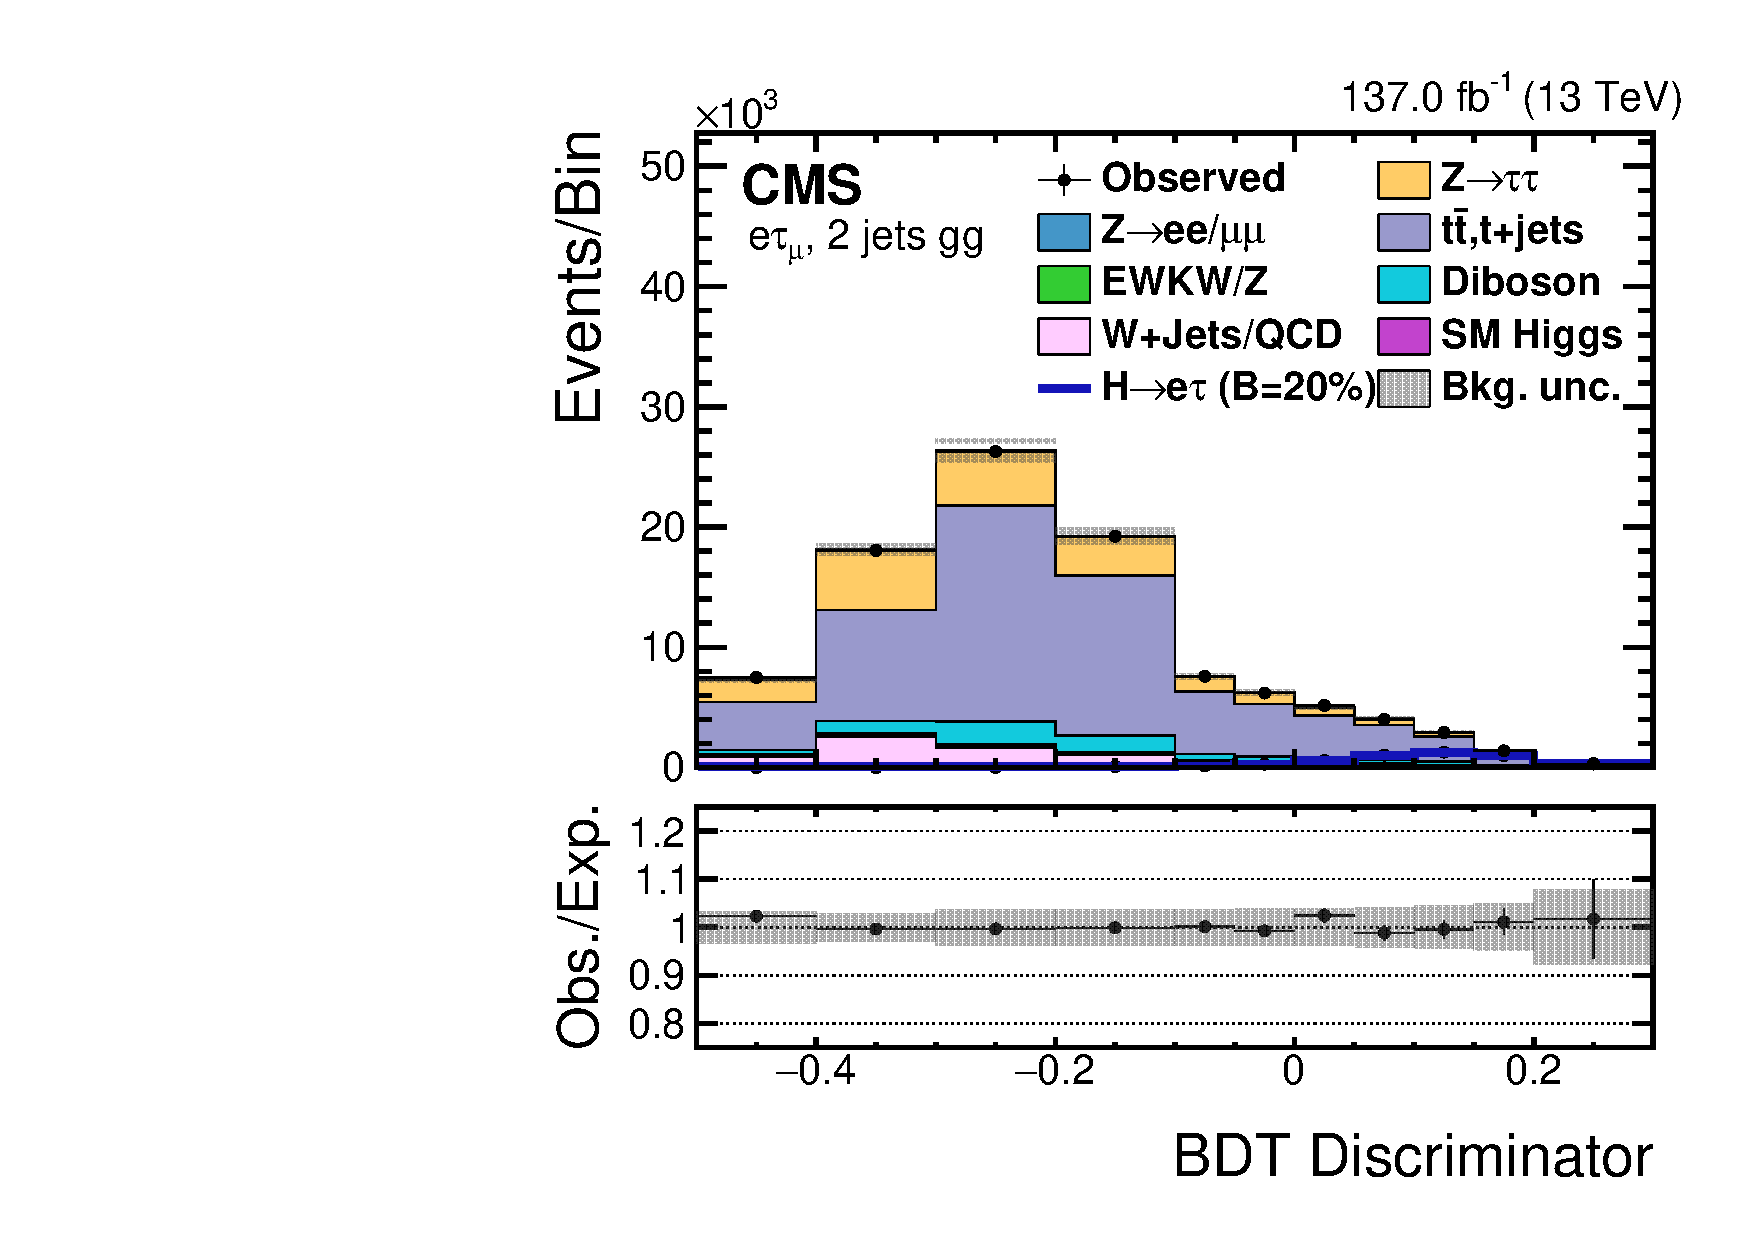
\includegraphics[width=0.4\textwidth]{plots/chapter9/BDT/emu/2jet_gg.pdf}
  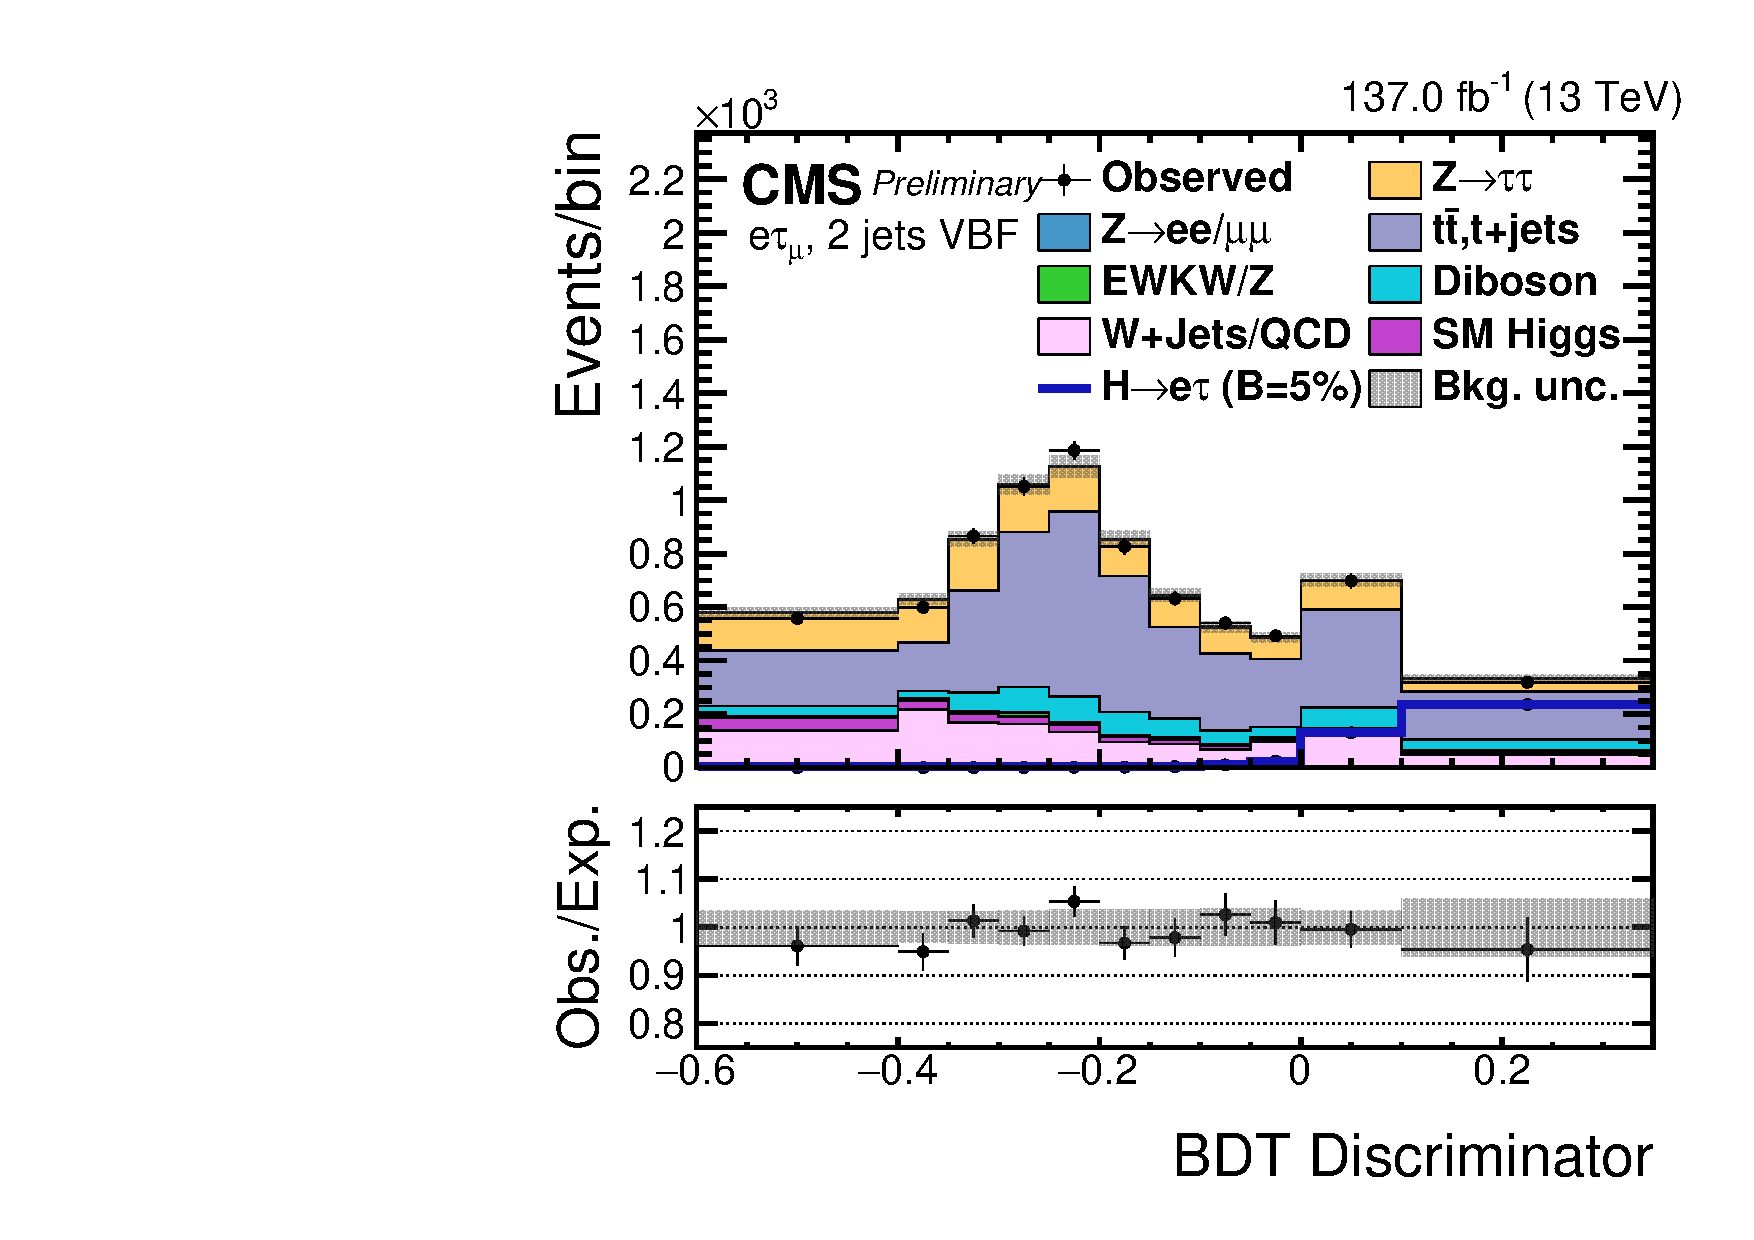
\includegraphics[width=0.4\textwidth]{plots/chapter9/BDT/emu/2jet_vbf.pdf} \\
  \caption{BDT discriminator distributions for the observed and estimated background in the \emu channel. The background is normalized to the best fit values from the signal plus background fit. Signal corresponds to \BHet = 20\%. The \emu channel categories are 0 jets (top left), 1 jet (top right), 2 jets gg (bottom left), and 2 jets VBF (bottom right). The bottom panel in each plot shows the fractional difference between the observed and estimated background. The uncertainty band shows the statistical and systematic uncertainties added in quadrature.}
  \label{fig:bdt_emu}
\end{figure}

\begin{figure}[htbp!]
  \centering
  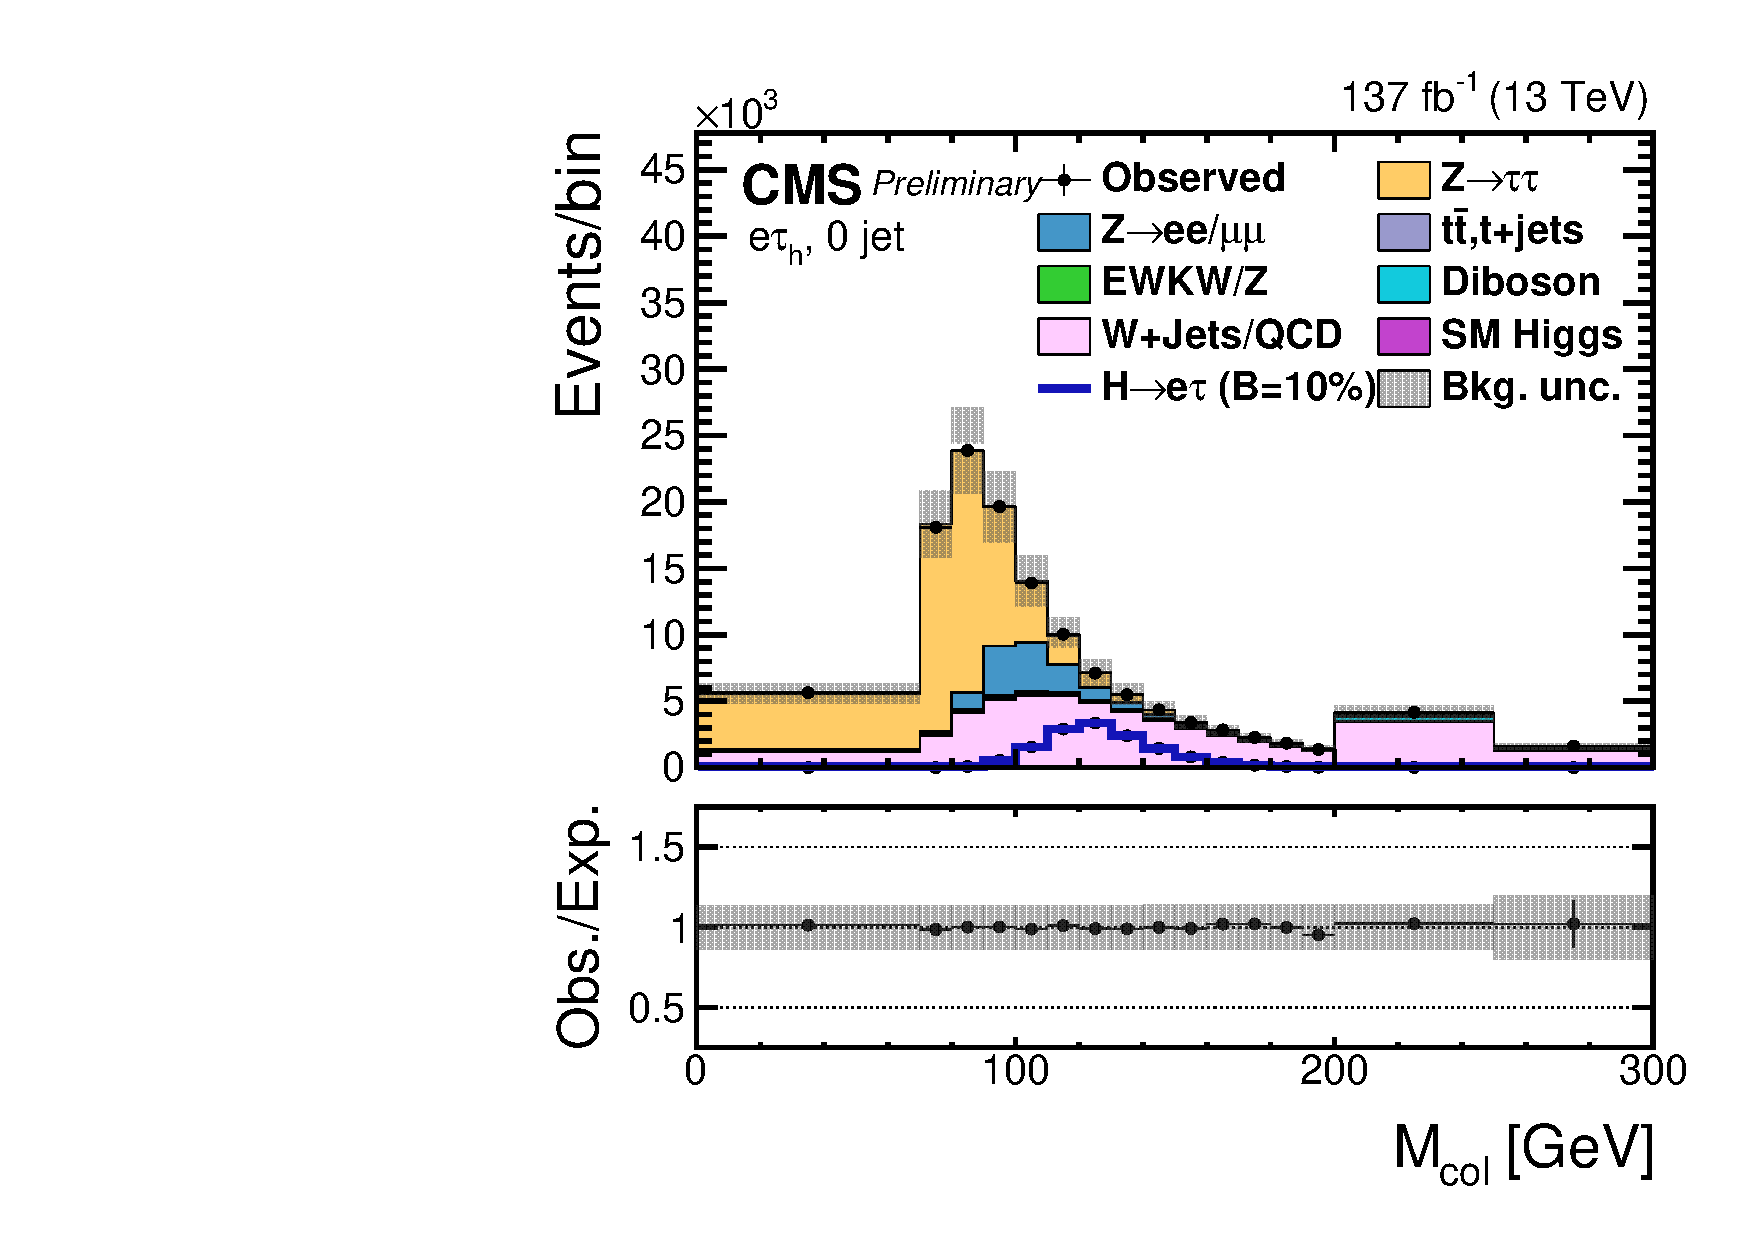
\includegraphics[width=0.4\textwidth]{plots/chapter9/CB/etau/0jet.pdf}
  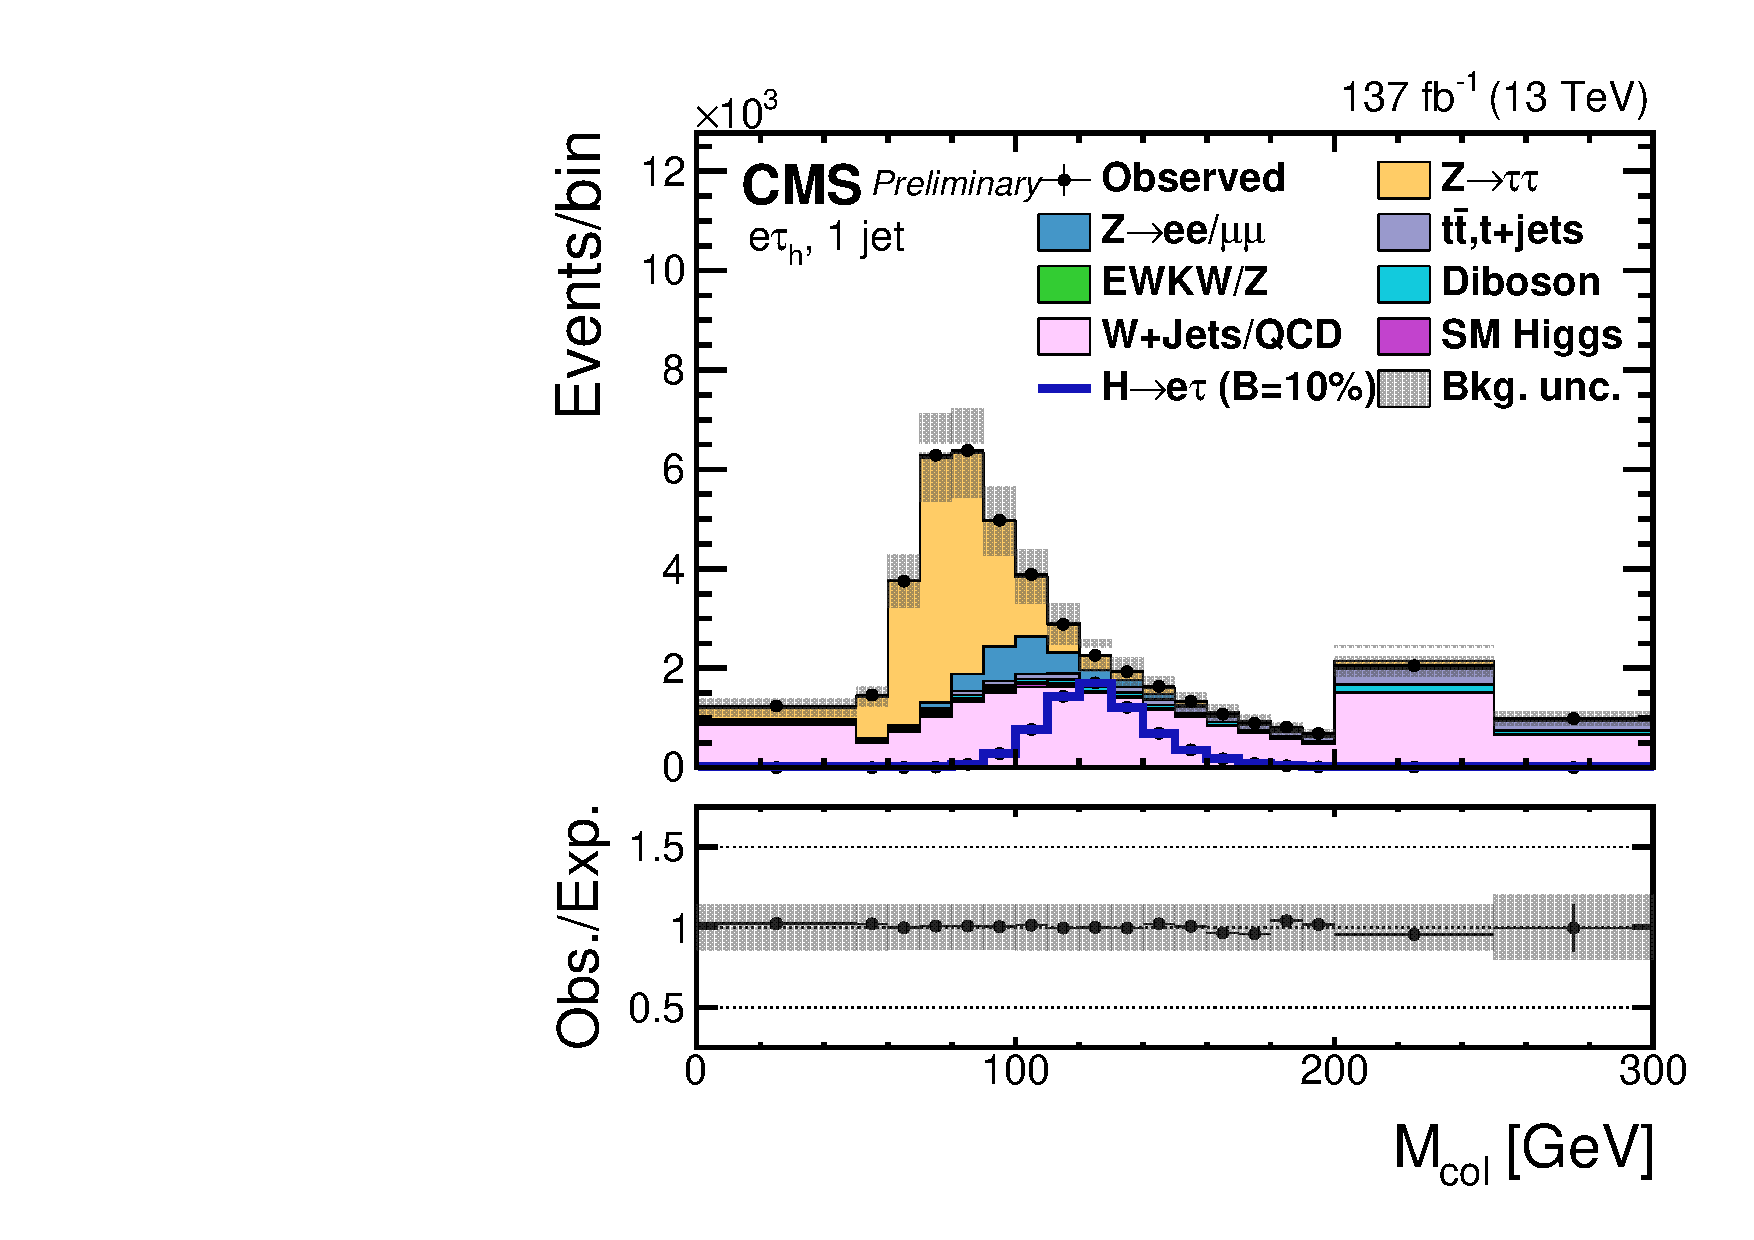
\includegraphics[width=0.4\textwidth]{plots/chapter9/CB/etau/1jet.pdf} \\
  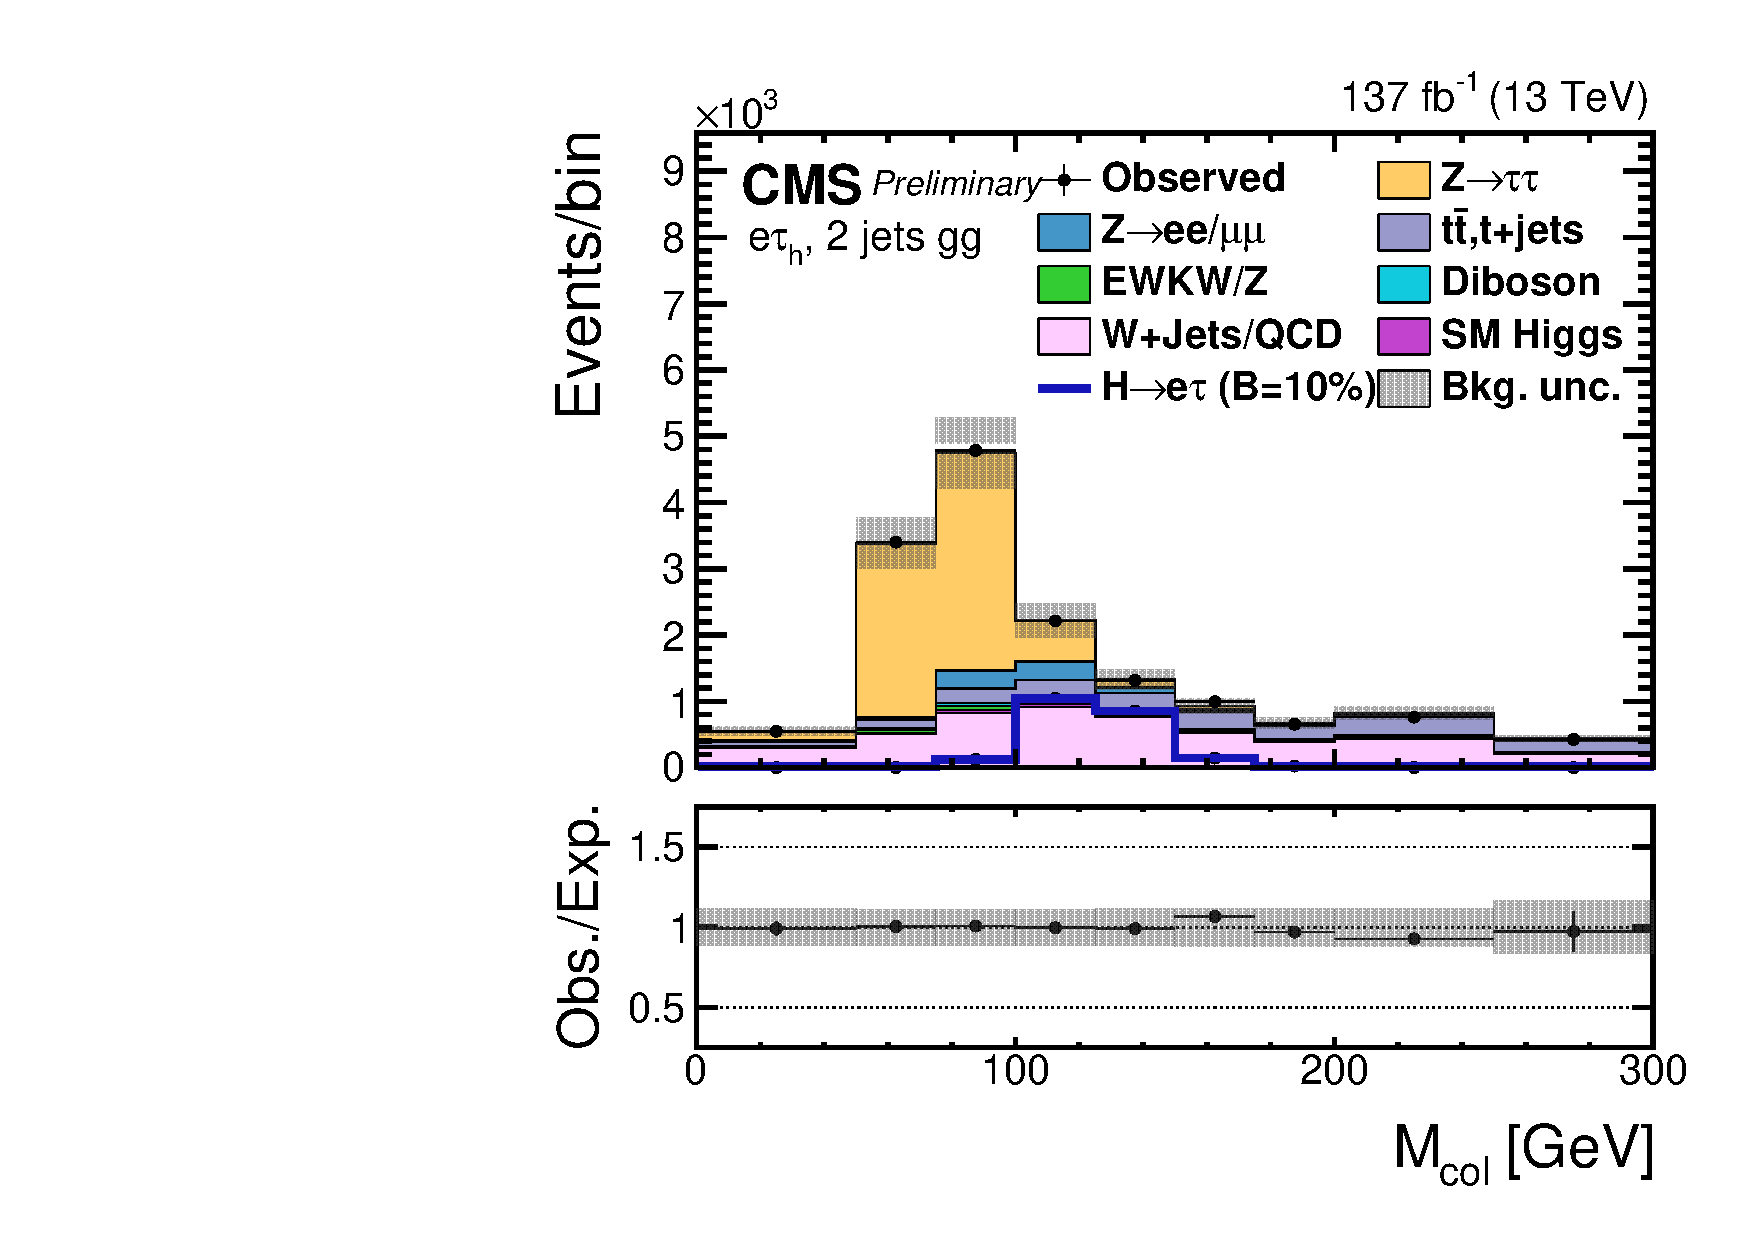
\includegraphics[width=0.4\textwidth]{plots/chapter9/CB/etau/2jet_gg.pdf}
  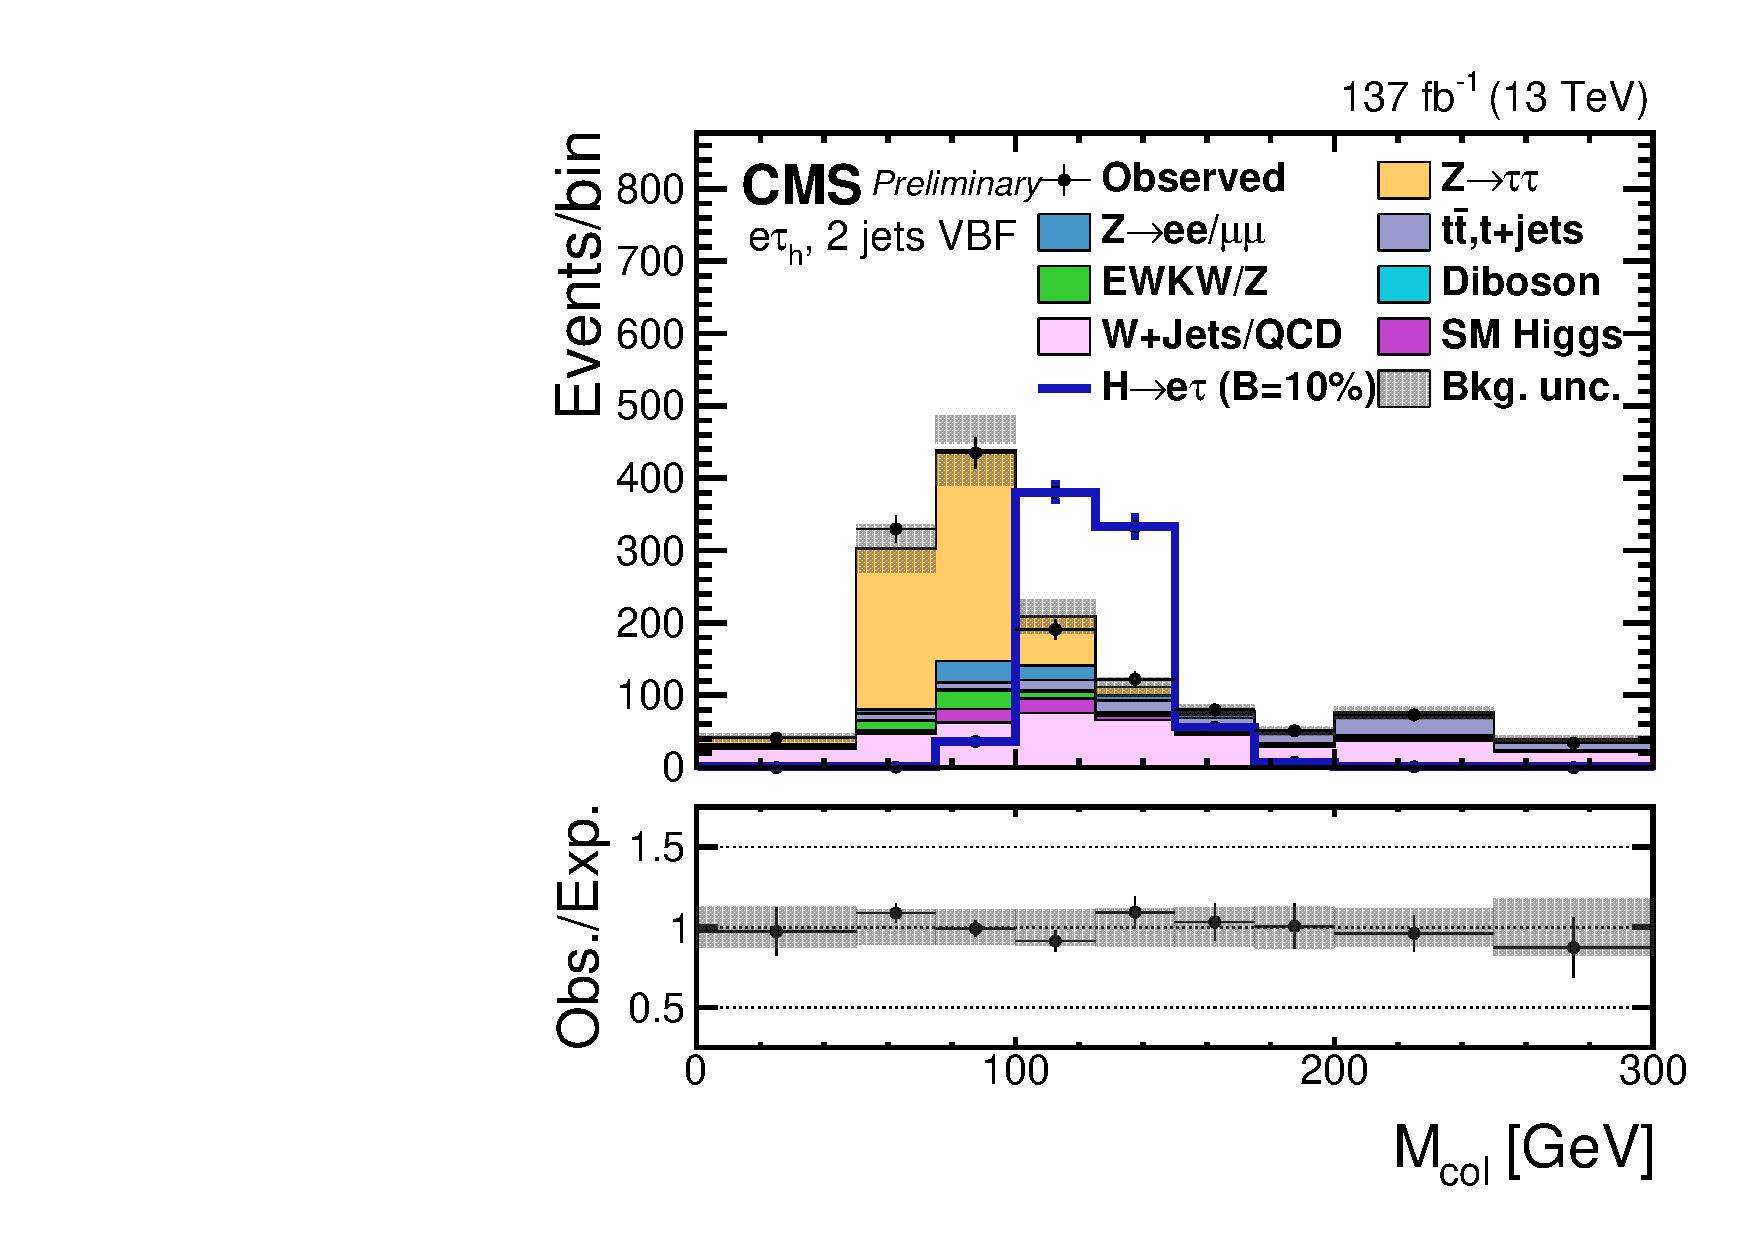
\includegraphics[width=0.4\textwidth]{plots/chapter9/CB/etau/2jet_vbf.pdf} \\
  \caption{\mcol distributions for the observed and estimated background in the \ehad channel. The background is normalized to the best fit values from the signal plus background fit. Signal corresponds to \BHet = 10\%. The \ehad channel categories are 0 jets (top left), 1 jet (top right), 2 jets gg (bottom left), and 2 jets VBF (bottom right). The bottom panel in each plot shows the fractional difference between the observed and estimated background. The uncertainty band shows the statistical and systematic uncertainties added in quadrature.}
  \label{fig:mcol_ehad}
\end{figure}

\begin{figure}[htbp!]
  \centering
  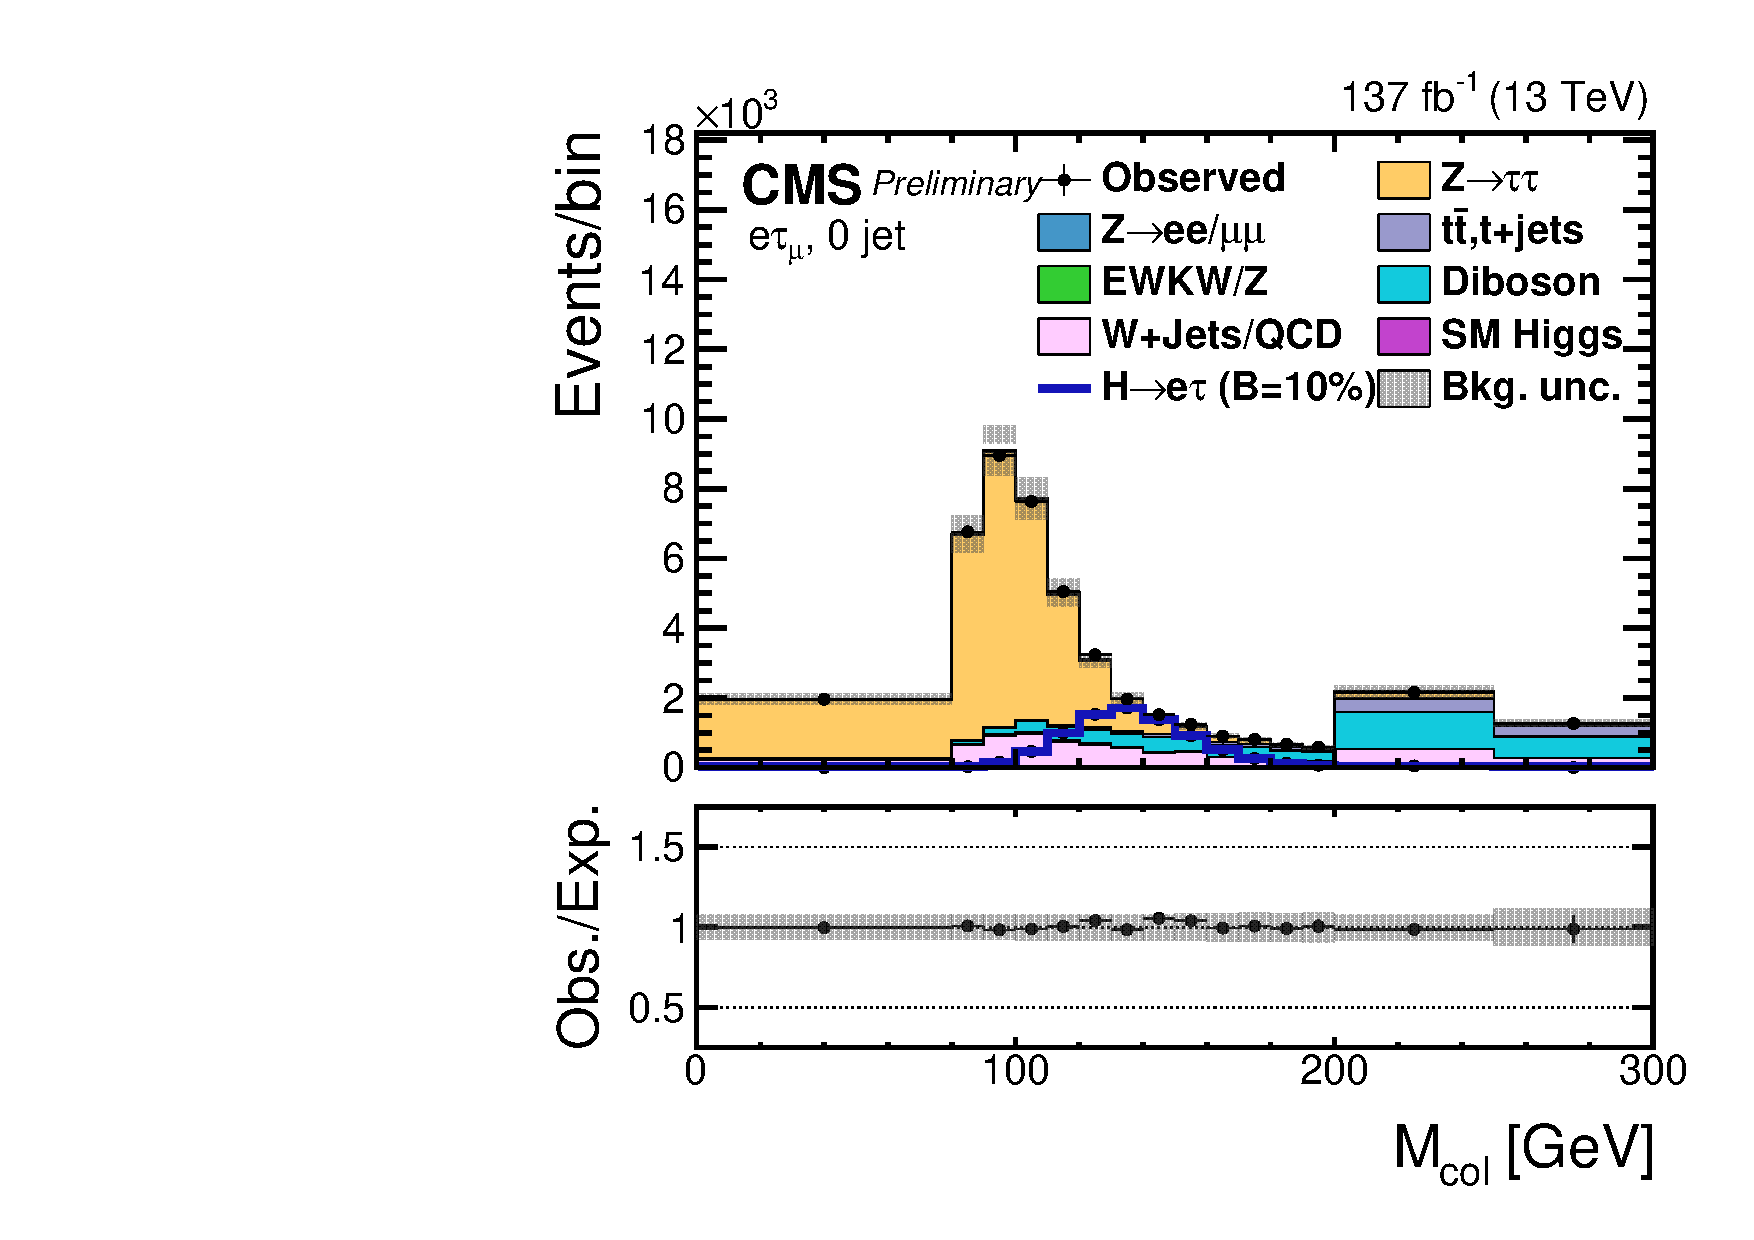
\includegraphics[width=0.4\textwidth]{plots/chapter9/CB/emu/0jet.pdf}
  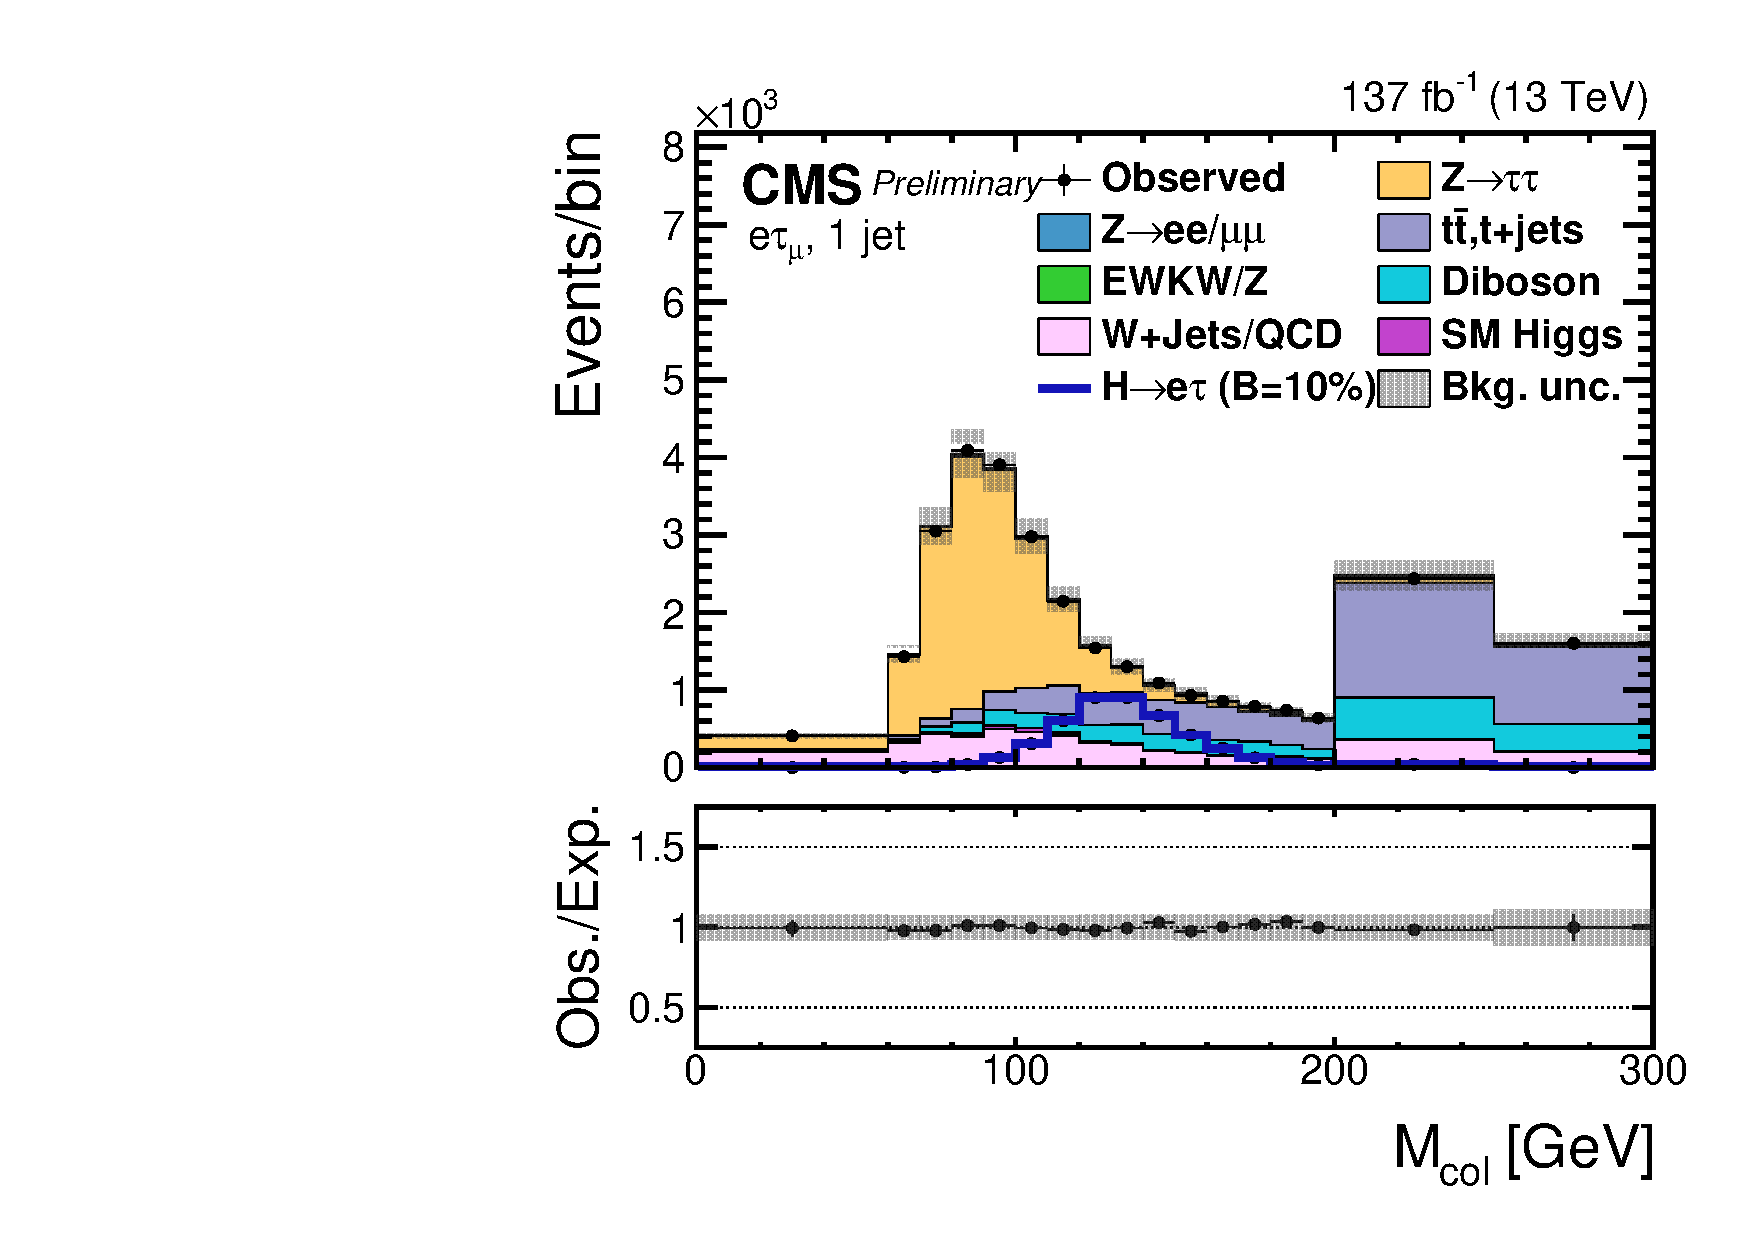
\includegraphics[width=0.4\textwidth]{plots/chapter9/CB/emu/1jet.pdf} \\
  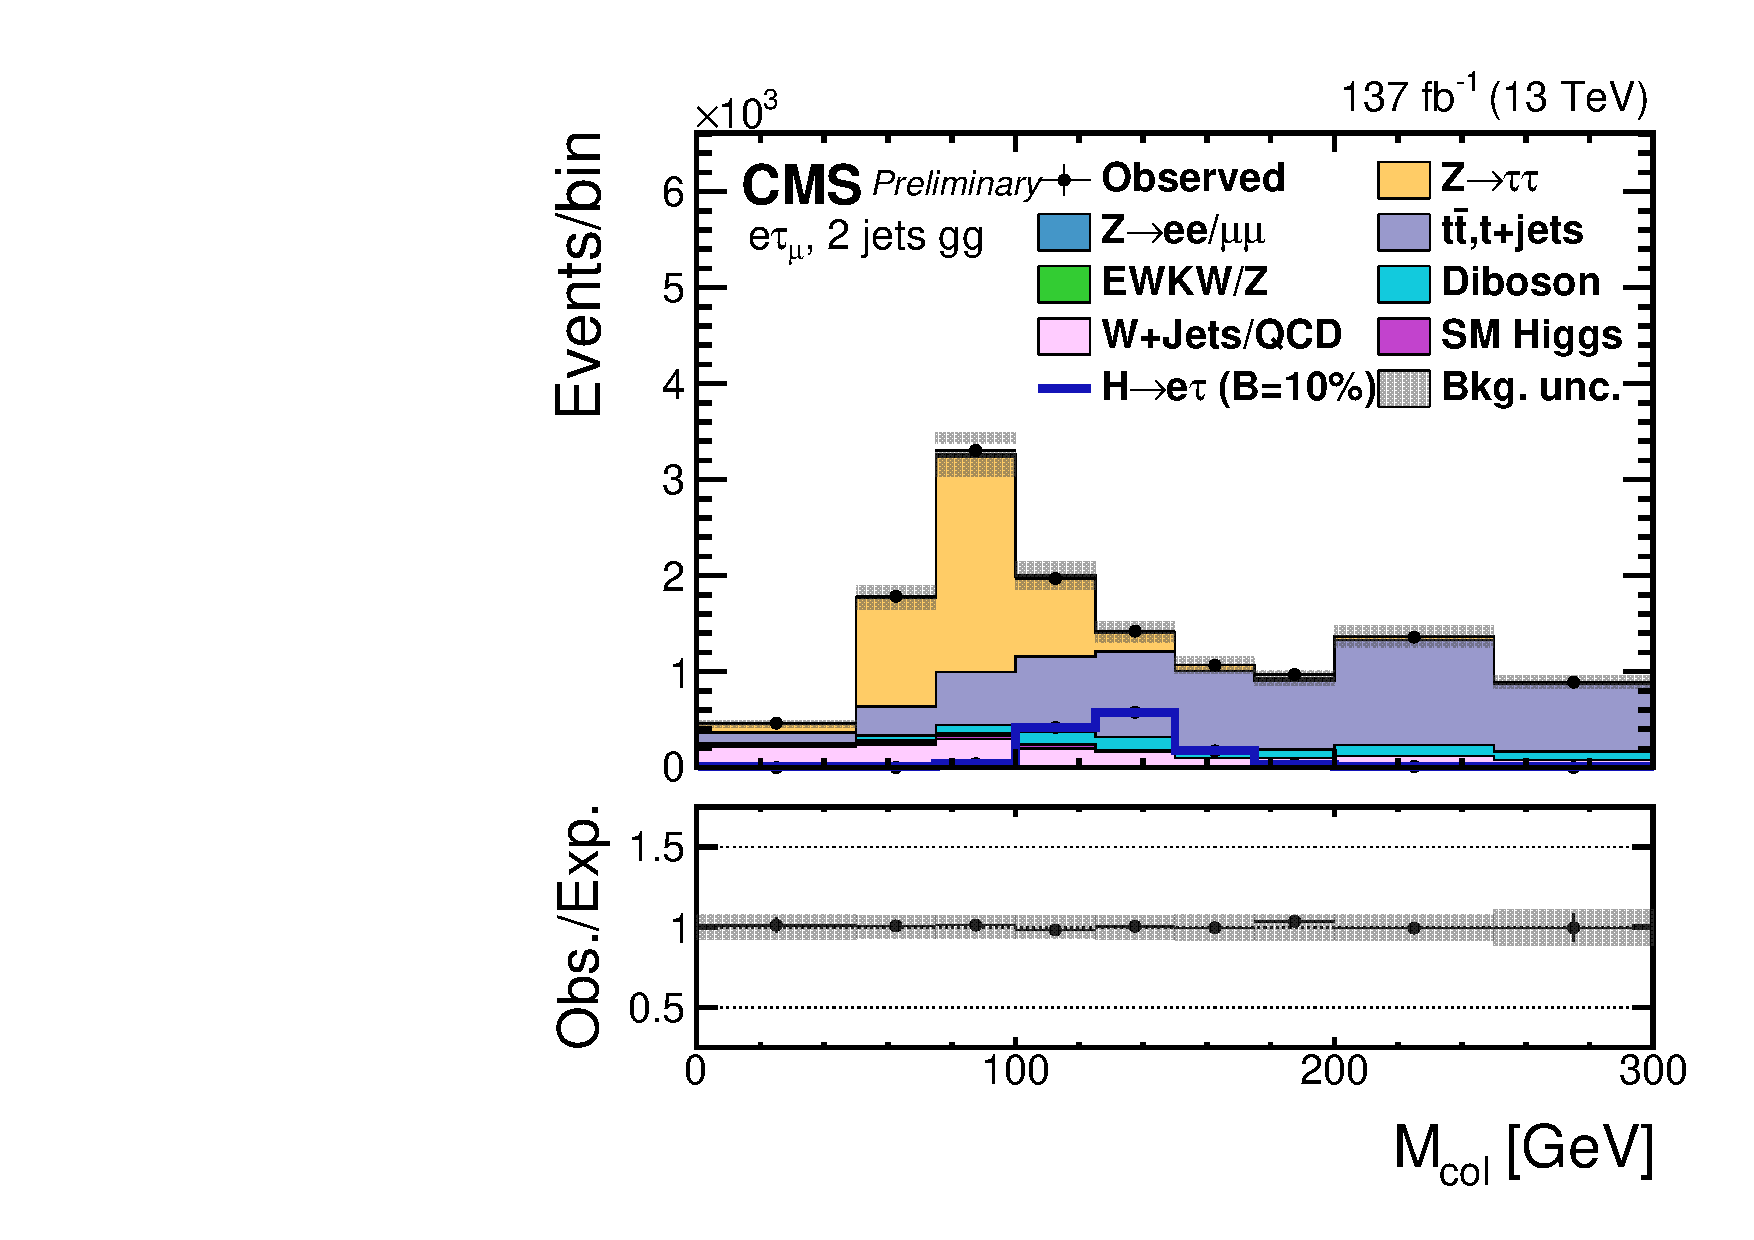
\includegraphics[width=0.4\textwidth]{plots/chapter9/CB/emu/2jet_gg.pdf}
  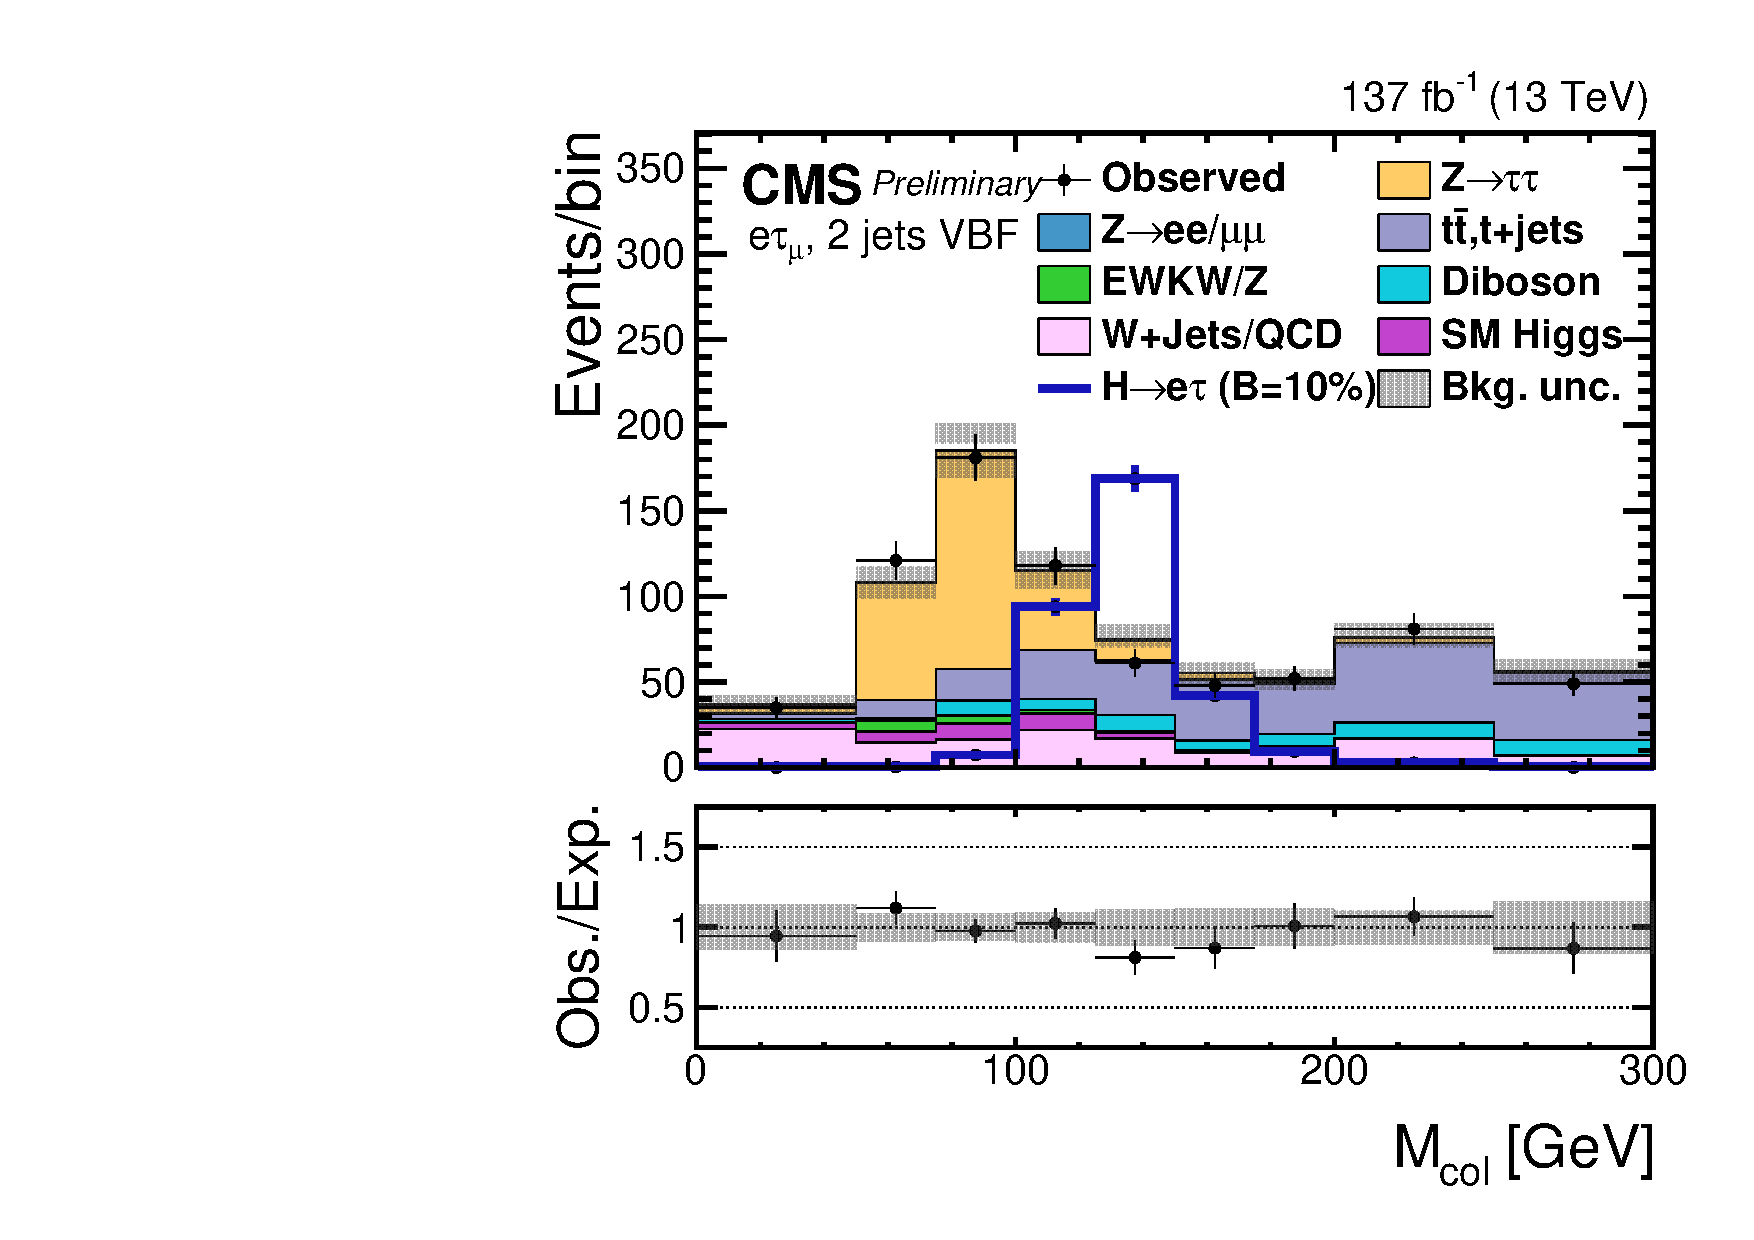
\includegraphics[width=0.4\textwidth]{plots/chapter9/CB/emu/2jet_vbf.pdf} \\
  \caption{\mcol distributions for the observed and estimated background in the \emu channel. The background is normalized to the best fit values from the signal plus background fit. Signal corresponds to \BHet = 10\%. The \emu channel categories are 0 jets (top left), 1 jet (top right), 2 jets gg (bottom left), and 2 jets VBF (bottom right). The bottom panel in each plot shows the fractional difference between the observed and estimated background. The uncertainty band shows the statistical and systematic uncertainties added in quadrature.}
  \label{fig:mcol_emu}
\end{figure}

The BDT analysis yields an observed (expected) upper limit on the Higgs branching fraction of 0.15\% (0.15\%) for \Hmt channel and 0.22\% (0.16\%) for \Het channel. The observed and median expected 95\% CL upper limits and the best fit branching fractions, for \BHmt and \BHet, assuming $\mh = 125 \GeV$, are reported in Tables~\ref{tab:limit_bdt_mutau} and~\ref{tab:limit_bdt_etau}. The limits are also summarized graphically in Figure~\ref{fig:bdt_limits} and in Table~\ref{tab:limits_summary}.

A cross-check analysis in which a maximum-likelihood fit is performed on the \mcol distribution after applying additional selections~\cite{Sirunyan:2017xzt} yields an observed (expected) upper limit on the Higgs branching fraction of 0.38\% (0.26\%) for \Hmt and 0.32\% (0.28\%) for \Het. The observed and median expected 95\% CL upper limits and the best fit branching fractions, for \BHmt and \BHet, assuming $\mh = 125 \GeV$, are reported in Tables~\ref{tab:limit_cb_mutau} and~\ref{tab:limit_cb_etau}. The BDT fit analysis is more sensitive than the \mcol fit analysis, and systematic uncertainties dominate results for both cases.

The upper limits on \BHmt and \BHet are subsequently used to put constraints on LFV Yukawa couplings~\cite{Harnik:2012pb}. The LFV decays \Pe{}\Pgt and \Pgm{}\Pgt arise at tree level from the assumed flavor violating Yukawa interactions, $\text{Y}_{\ell^\alpha\ell^{\beta}}$, where $\ell^\alpha, \ell^\beta$ are the leptons (\Pe, \Pgm, \Pgt) of different flavors ($\alpha\ne\beta$).

The decay width of LFV Higgs boson decays is
\begin{equation}
  \Gamma(\text{H} \to \ell_{i} \ell_{j})=\frac{\text{M}_{\text{H}}}{8 \pi}(|\text{Y}_{j i}|^2+|\text{Y}_{i j}|^2)
\end{equation}
using the decay width of the LFV decay, the branching fraction of the LFV Higgs boson decay can be derived when contributions of the other LFV decays are negligible
\begin{equation}
  \mathcal{B}(\text{H} \to \ell_{i} \ell_{j})=\frac{\Gamma(\text{H} \to \ell_{i} \ell_{j})}{\Gamma(\text{H} \to \ell_{i} \ell_{j})+\Gamma_{\text{SM}}}
\end{equation}
where \gsm is the total width of the Higgs boson in the SM. Non-negligible contributions to the total decay width from other LFV Higgs boson decays would have to be added to \gsm for estimating the branching fractions.

The SM Higgs boson decay width is assumed to be $\Gamma_{\text{SM}} = 4.1~\MeV$~\cite{Denner:2011mq} for $\mh = 125 \GeV$. The 95\% CL upper limit on the Yukawa couplings derived from the expression for the branching fraction above is shown in Table~\ref{tab:limits_summary}. The limits on the Yukawa couplings derived from the BDT fit analysis results are shown in Figure~\ref{fig:bdt_yukawa_limits}.

%%-----------------------------------
%% Limits:
%%-----------------------------------
\begin{figure}[htbp!]
  \centering
  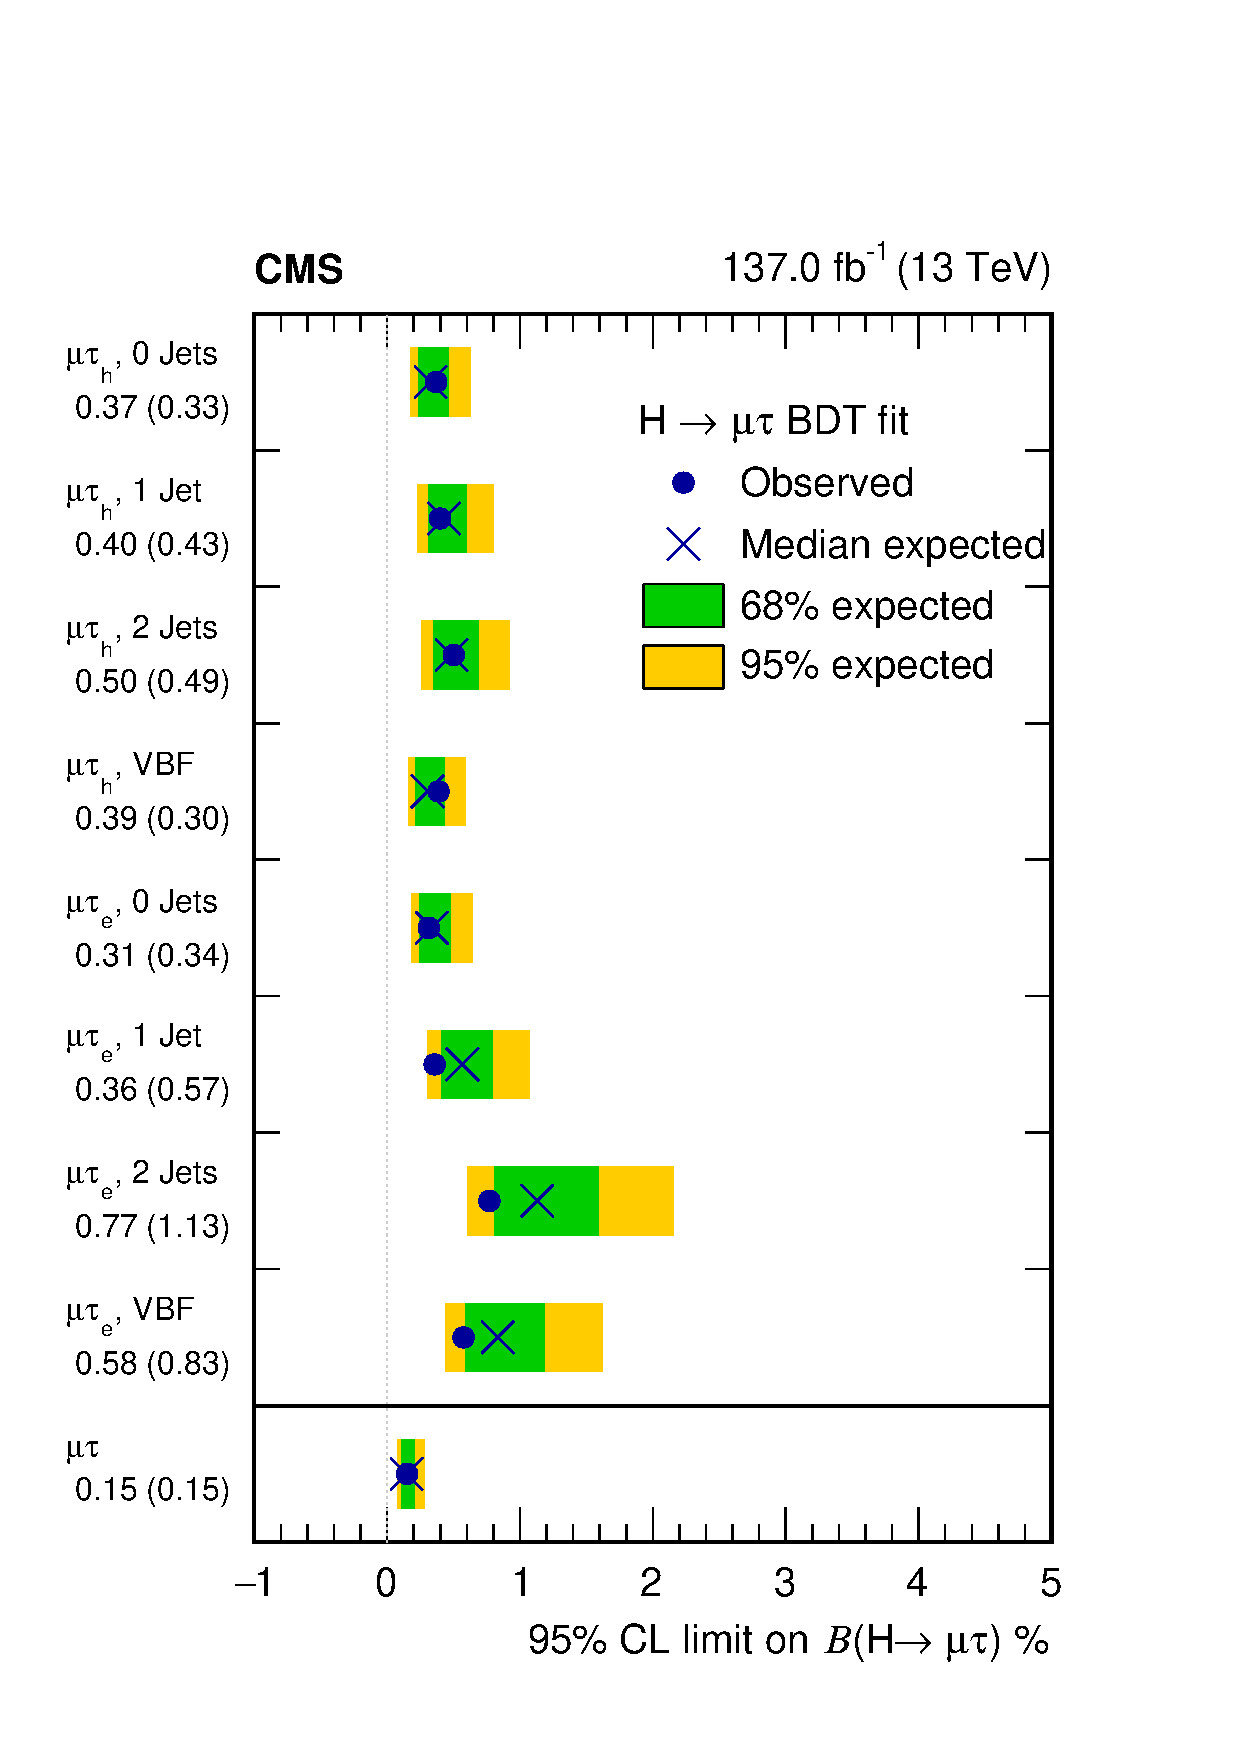
\includegraphics[width=0.45\textwidth]{plots/chapter9/limits/BDTMu.pdf}
  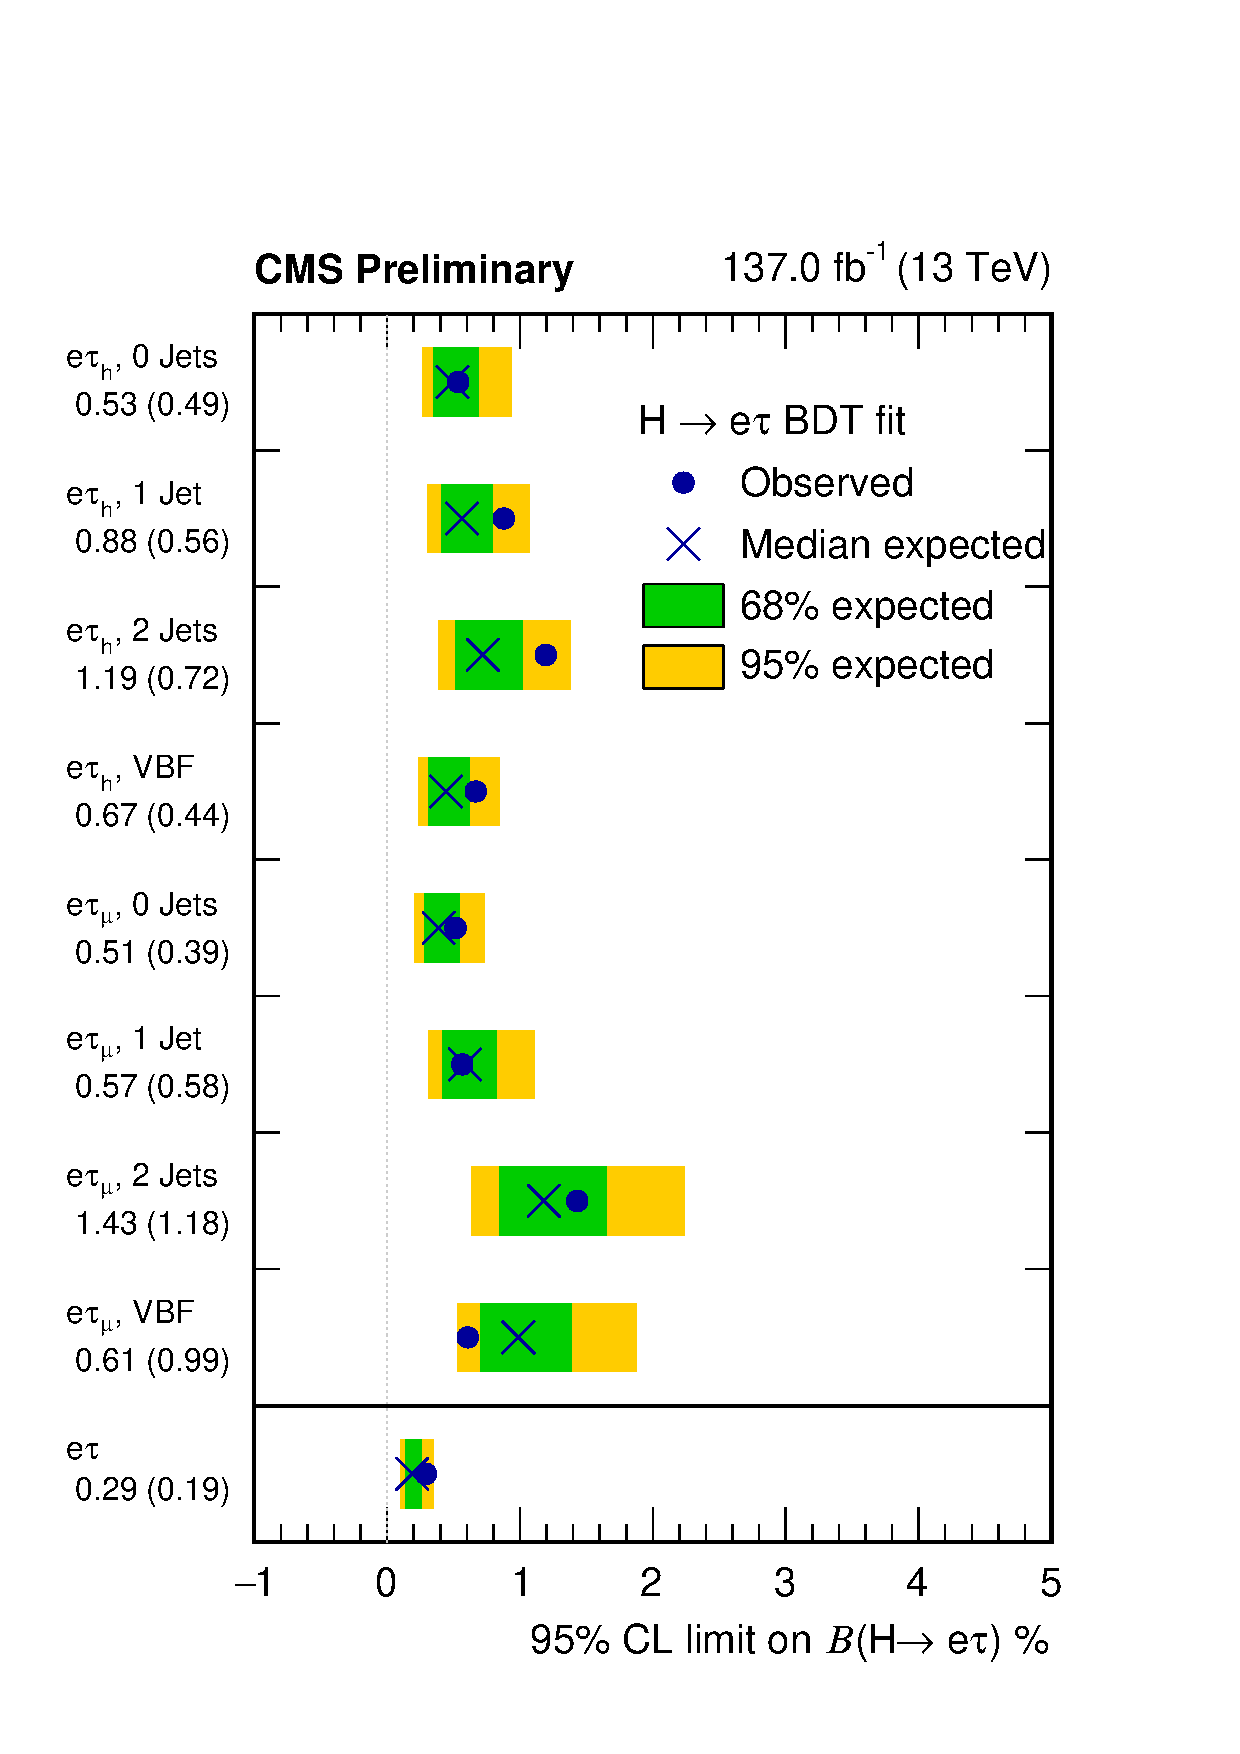
\includegraphics[width=0.45\textwidth]{plots/chapter9/limits/BDTE.pdf} \\
  \caption{Observed (expected) 95\% CL upper limits on the \BHmt (left) and \BHet (right) for each individual category and combined from the BDT fit analysis.}
  \label{fig:bdt_limits}
\end{figure}

% \begin{figure}[htbp!]
%   \centering
%   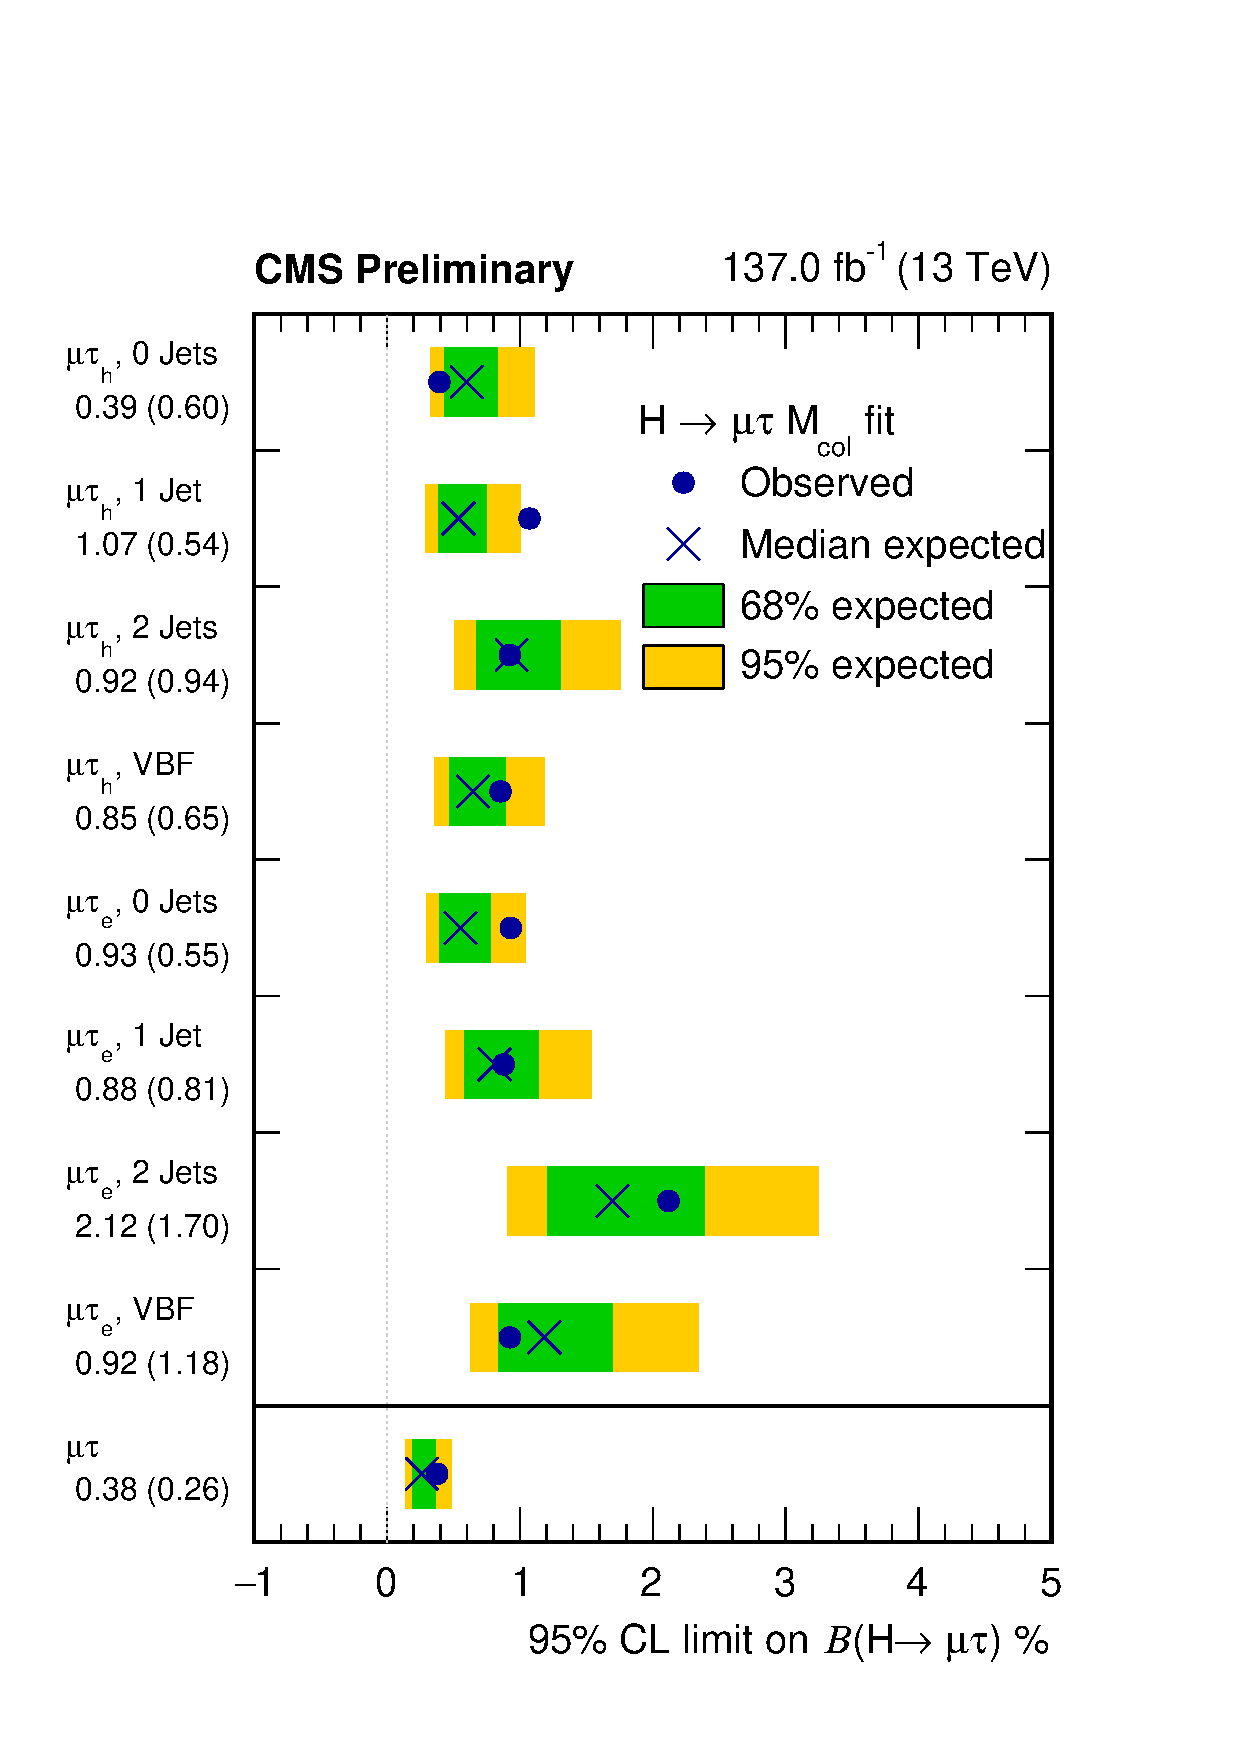
\includegraphics[width=0.45\textwidth]{plots/chapter9/limits/CBMu.pdf}
%   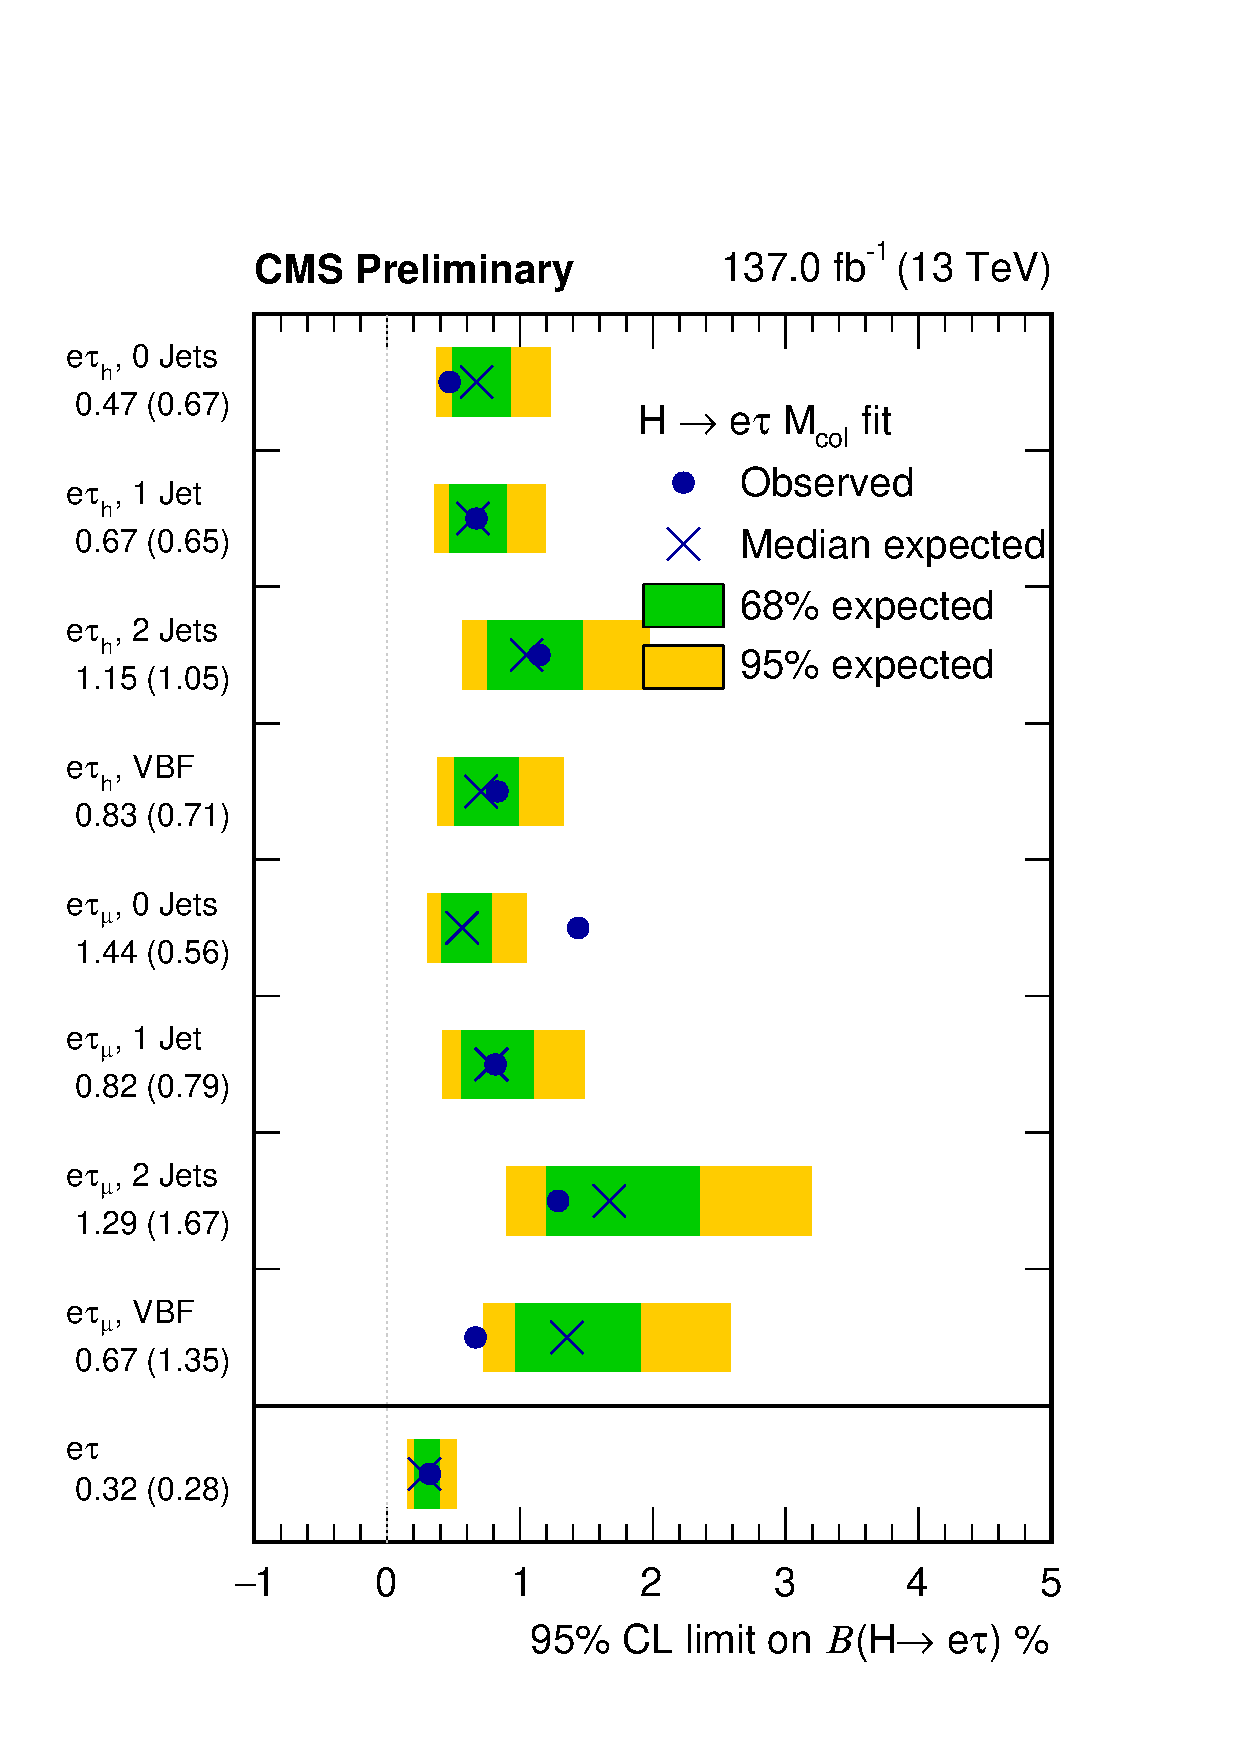
\includegraphics[width=0.45\textwidth]{plots/chapter9/limits/CBE.pdf} \\
%   \caption{Observed (expected) 95\% CL upper limits on the \BHmt (left) and \BHet (right) for each individual category and combined from the \mcol fit analysis.}
%   \label{fig:cb_limits}
% \end{figure}

%%-----------------------------------
%% Yukawa Limits:
%%-----------------------------------
\begin{figure}[htbp!]
  \centering
  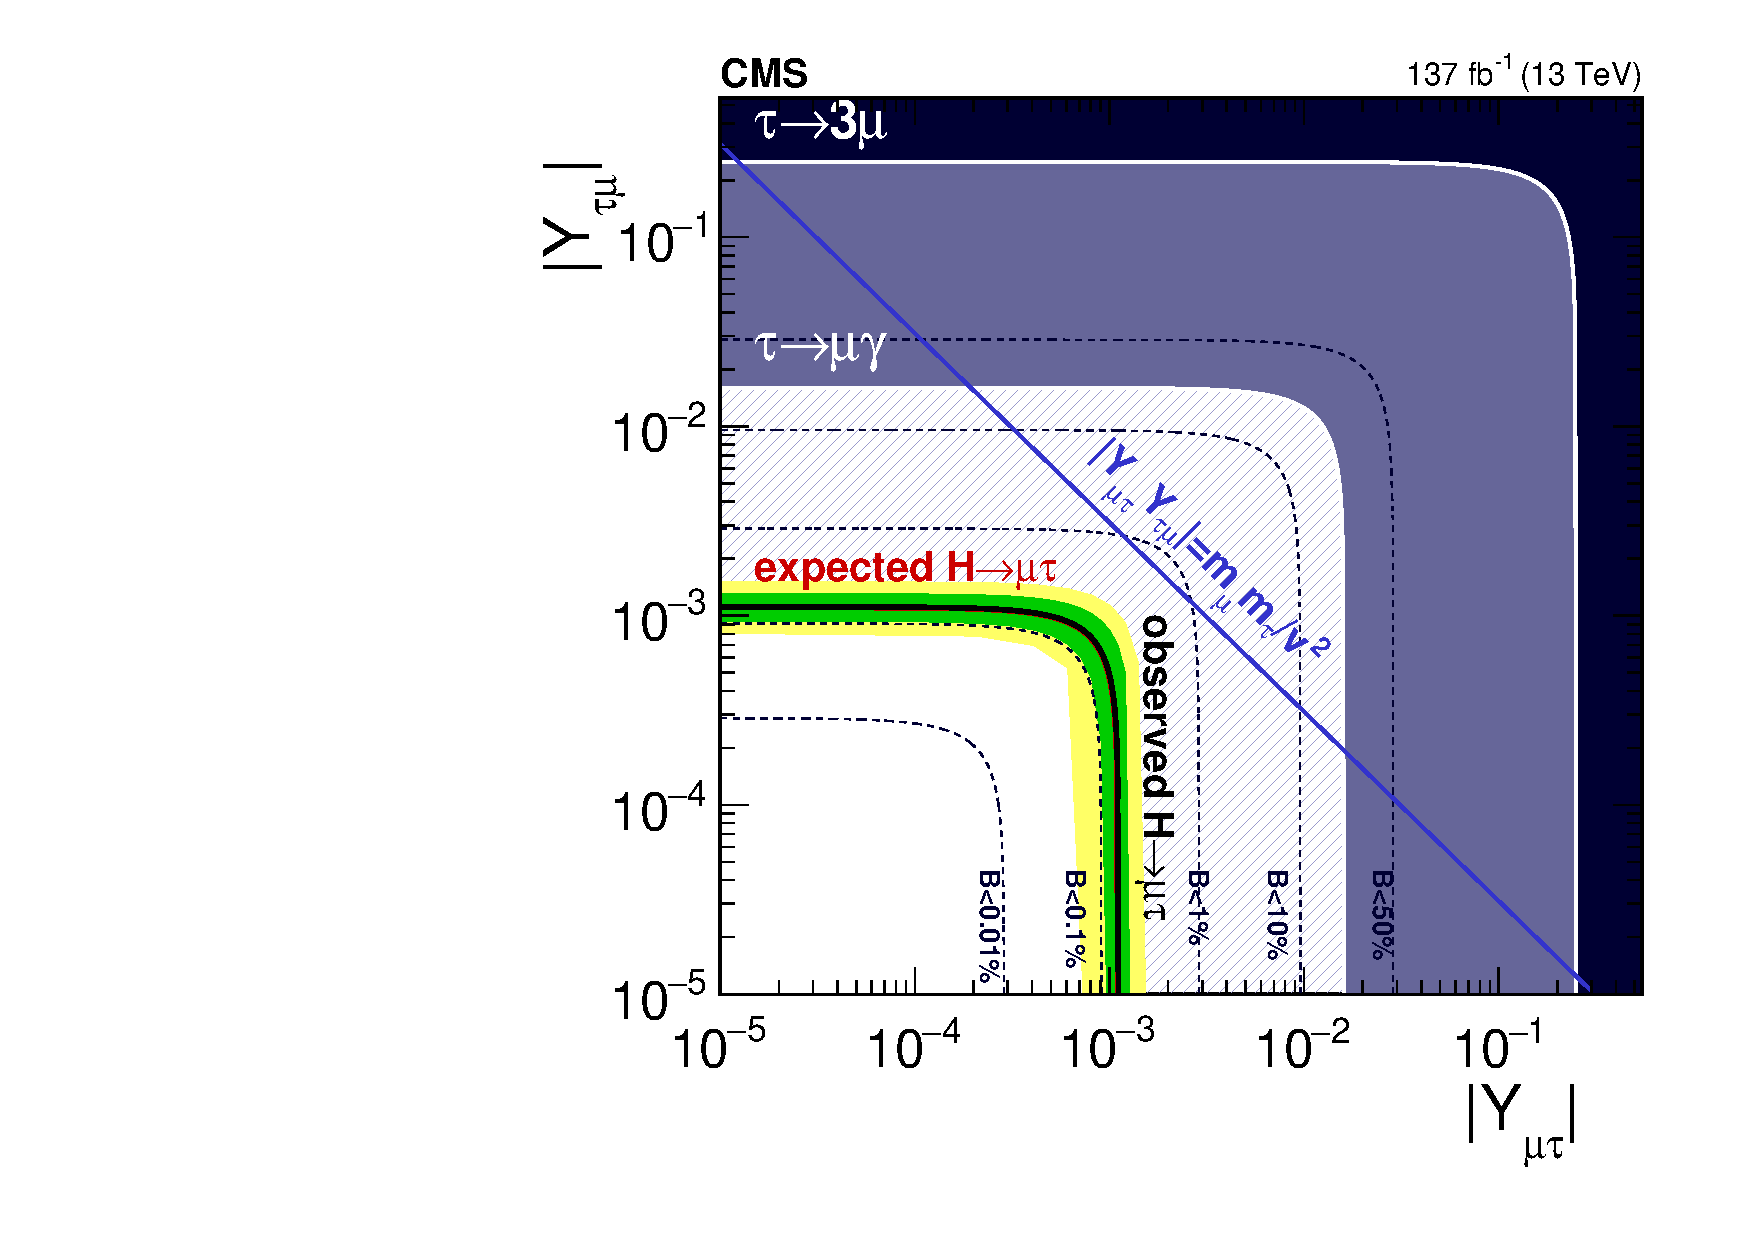
\includegraphics[width=0.45\textwidth]{plots/chapter9/limits/Ymt.pdf}
  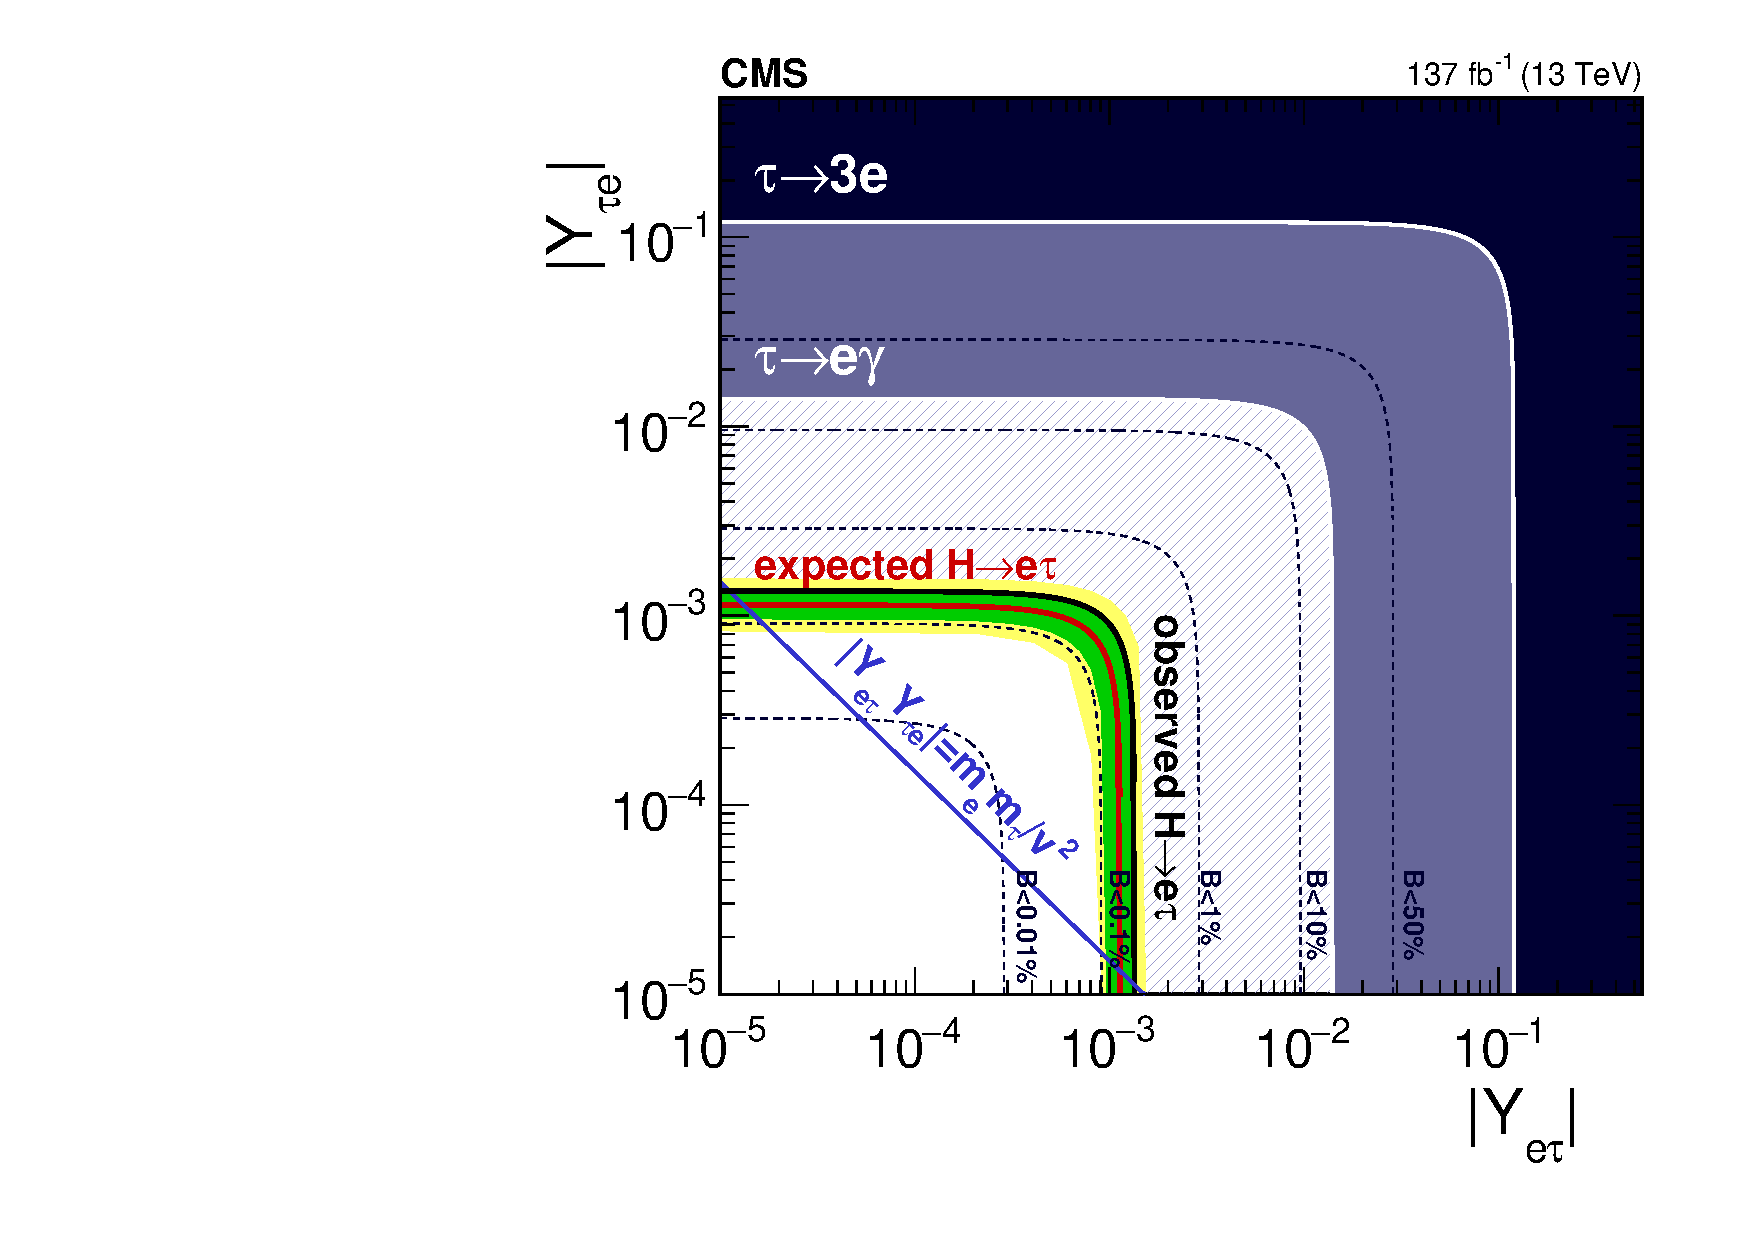
\includegraphics[width=0.45\textwidth]{plots/chapter9/limits/Yet.pdf} \\
  \caption{Constraints on the LFV Yukawa couplings, $\Ymutau-\Ytaumu$ (left), and $\Yetau-\Ytaue$ (right). The expected (red line) and observed (black solid line) limits are derived from the results shown in Figure~\ref{fig:bdt_limits}. The flavor-diagonal Yukawa couplings are approximated by their SM values. The green hashed region is derived by the CMS direct search presented in this dissertation. The green (yellow) band indicates the range that is expected to contain 68\% (95\%) of all observed limit variations from the expected limit. The shaded regions are derived constraints from null searches for $\Pgt\to3\Pgm$ or $\Pgt\to3\Pe$ (dark green)~\cite{Hayasaka:2010np} and $\Pgt\to\Pgm\Pgg$ or $\Pgt\to\Pe\Pgg$ (lighter green)~\cite{Harnik:2012pb}. The blue diagonal line is the theoretical naturalness limit $|\text{Y}_{ij}\text{Y}_{ji}|\leq{\text{m}_i}\text{m}_j/v^2$.}
  \label{fig:bdt_yukawa_limits}
\end{figure}

\begin{table}[!hbpt]
\centering
\caption{Observed and expected upper limits at 95\% CL and best fit branching fractions for each individual jet category, and combined, in the \Hmt process.}
\begin{tabular}{cccccc}
\hline
\multicolumn{6}{c}{Expected limits (\%)}                           \\
\hline
       & 0-jet     & 1-jet     & 2-jets    & VBF       & Combined  \\
\cline{2-6}
\mue   & $<$ 0.36  & $<$ 0.56  & $<$ 1.13   & $<$ 0.93 & $<$ 0.28  \\
\muhad & $<$ 0.34  & $<$ 0.45  & $<$ 0.53   & $<$ 0.32 & $<$ 0.19  \\
\cline{2-6}
\mutau & \multicolumn{5}{c}{$<$ 0.16}                              \\
\hline
\multicolumn{6}{c}{Observed limits (\%)}                           \\
\hline
       & 0-jet     & 1-jet     & 2-jets    & VBF       & Combined  \\
\cline{2-6}
\mue   & $<$ 0.27  & $<$ 0.35  & $<$ 0.79   & $<$ 0.60 & $<$ 0.17  \\
\muhad & $<$ 0.40  & $<$ 0.43  & $<$ 0.58   & $<$ 0.44 & $<$ 0.27  \\
\cline{2-6}
\mutau & \multicolumn{5}{c}{$<$ 0.15}                              \\
\hline
\multicolumn{6}{c}{Best fit branching fractions (\%)}              \\
\hline
       & 0-jet     & 1-jet     & 2-jets    & VBF       & Combined  \\
\cline{2-6}
\mue   & -0.16 $\pm$ 0.18 & -0.41 $\pm$ 0.28 & -0.61 $\pm$ 0.57 & -0.58 $\pm$ 0.44 & -0.22 $\pm$ 0.14 \\
\muhad & 0.09 $\pm$ 0.17  & -0.03 $\pm$ 0.23 & 0.08 $\pm$ 0.27  & 0.15 $\pm$ 0.16  & 0.10 $\pm$ 0.10  \\
\cline{2-6}
\mutau & \multicolumn{5}{c}{-0.01 $\pm$ 0.08}                                                         \\
\hline
\end{tabular}
\label{tab:limit_bdt_mutau}
\end{table}

\begin{table}[!hbpt]
\centering
\caption{Observed and expected upper limits at 95\% CL and best fit branching fractions for each individual jet category, and combined, in the \Het process.}
\begin{tabular}{cccccc}
\hline
\multicolumn{6}{c}{Expected limits (\%)}                          \\
\hline
      & 0-jet     & 1-jet     & 2-jets    & VBF       & Combined  \\
\cline{2-6}
\emu  & $<$ 0.39  & $<$ 0.58  & $<$ 1.18  & $<$ 0.99  & $<$ 0.29  \\
\ehad & $<$ 0.49  & $<$ 0.56  & $<$ 0.72  & $<$ 0.44  & $<$ 0.25  \\
\cline{2-6}
\etau & \multicolumn{5}{c}{$<$ 0.19}                              \\
\hline
\multicolumn{6}{c}{Observed limits (\%)}                          \\
\hline
      & 0-jet     & 1-jet     & 2-jets    & VBF       & Combined  \\
\cline{2-6}
\emu  & $<$ 0.51  & $<$ 0.57  & $<$ 1.43  & $<$ 0.61  & $<$ 0.31  \\
\ehad & $<$ 0.53  & $<$ 0.88  & $<$ 1.19  & $<$ 0.67  & $<$ 0.45  \\
\cline{2-6}
\etau & \multicolumn{5}{c}{$<$ 0.29}                              \\
\hline
\multicolumn{6}{c}{Best fit branching fractions (\%)}             \\
\hline
      & 0-jet     & 1-jet     & 2-jets    & VBF       & Combined  \\
\cline{2-6}
\emu  & 0.17 $\pm$ 0.20  & -0.03 $\pm$ 0.29 & 0.33 $\pm$ 0.60  & -0.73 $\pm$ 0.58 & 0.02 $\pm$ 0.15  \\
\ehad & 0.06 $\pm$ 0.25  & 0.38 $\pm$ 0.29  & 0.57 $\pm$ 0.37  & 0.28 $\pm$ 0.12  & 0.23 $\pm$ 0.13  \\
\cline{2-6}
\etau & \multicolumn{5}{c}{0.13 $\pm$ 0.10}                                                          \\
\hline
\end{tabular}
\label{tab:limit_bdt_etau}
\end{table}

\begin{table}[!hbpt]
\centering
\caption{Observed and expected upper limits at 95\% CL and best fit branching fractions for each individual jet category, and combined, in the \Hmt process from \mcol fit analysis.}
\begin{tabular}{cccccc}
\hline
\multicolumn{6}{c}{Expected limits (\%)}                           \\
\hline
       & 0-jet     & 1-jet     & 2-jets    & VBF       & Combined  \\
\cline{2-6}
\mue   & $<$ 0.55  & $<$ 0.81  & $<$ 1.70  & $<$ 1.18  & $<$ 0.42  \\
\muhad & $<$ 0.60  & $<$ 0.54  & $<$ 0.94  & $<$ 0.65  & $<$ 0.34  \\
\cline{2-6}
\mutau & \multicolumn{5}{c}{$<$ 0.26}                              \\
\hline
\multicolumn{6}{c}{Observed limits (\%)}                           \\
\hline
       & 0-jet     & 1-jet     & 2-jets    & VBF       & Combined  \\
\cline{2-6}
\mue   & $<$ 0.93  & $<$ 0.88  & $<$ 2.12  & $<$ 0.92  & $<$ 0.60  \\
\muhad & $<$ 0.39  & $<$ 1.07  & $<$ 0.92  & $<$ 0.85  & $<$ 0.46  \\
\cline{2-6}
\mutau & \multicolumn{5}{c}{$<$ 0.38}                              \\
\hline
\multicolumn{6}{c}{Best fit branching fractions (\%)}              \\
\hline
      & 0-jet     & 1-jet     & 2-jets    & VBF       & Combined   \\
\cline{2-6}
\mue   & 0.45 $\pm$ 0.29  & 0.08 $\pm$ 0.42  & 0.56 $\pm$ 0.85  & -0.35 $\pm$ 0.55 & 0.23 $\pm$ 0.21 \\
\muhad & -0.42 $\pm$ 0.32 & 0.62 $\pm$ 0.27  & -0.02 $\pm$ 0.48 & 0.29 $\pm$ 0.33  & 0.16 $\pm$ 0.17 \\
\cline{2-6}
\mutau & \multicolumn{5}{c}{ 0.15 $\pm$ 0.13 }                                                       \\
\hline
\end{tabular}
\label{tab:limit_cb_mutau}
\end{table}

\begin{table}[!hbpt]
\centering
\caption{Observed and expected upper limits at 95\% CL and best fit branching fractions for each individual jet category, and combined, in the \Het process from \mcol fit analysis.}
\begin{tabular}{cccccc}
\hline
\multicolumn{6}{c}{Expected limits (\%)}                          \\
\hline
      & 0-jet     & 1-jet     & 2-jets    & VBF       & Combined  \\
\cline{2-6}
\emu  & $<$ 0.56  & $<$ 0.79  & $<$ 1.67  & $<$ 1.35  & $<$ 0.44  \\
\ehad & $<$ 0.67  & $<$ 0.65  & $<$ 1.05  & $<$ 0.71  & $<$ 0.38  \\
\cline{2-6}
\etau & \multicolumn{5}{c}{$<$ 0.28}                              \\
\hline
\multicolumn{6}{c}{Observed limits (\%)}                          \\
\hline
      & 0-jet     & 1-jet     & 2-jets    & VBF       & Combined  \\
\cline{2-6}
\emu  & $<$ 1.44  & $<$ 0.82  & $<$ 1.29  & $<$ 0.67  & $<$ 0.65  \\
\ehad & $<$ 0.47  & $<$ 0.67  & $<$ 1.15  & $<$ 0.83  & $<$ 0.34  \\
\cline{2-6}
\etau & \multicolumn{5}{c}{$<$ 0.32}                              \\
\hline
\multicolumn{6}{c}{Best fit branching fractions (\%)}             \\
\hline
      & 0-jet     & 1-jet     & 2-jets    & VBF       & Combined  \\
\cline{2-6}
\emu  & 0.96 $\pm$ 0.29  & 0.04 $\pm$ 0.40  & -0.66 $\pm$ 0.84 & -1.64 $\pm$ 0.68 & 0.26 $\pm$ 0.23  \\
\ehad & -0.45 $\pm$ 0.39 & 0.04 $\pm$ 0.34  & 0.14 $\pm$ 0.53  & 0.17 $\pm$ 0.37  & -0.08 $\pm$ 0.20 \\
\cline{2-6}
\etau & \multicolumn{5}{c}{0.05 $\pm$ 0.14}                                                          \\
\hline
\end{tabular}
\label{tab:limit_cb_etau}
\end{table}

\begin{table}
\centering
\caption{Summary of observed and expected upper limits at 95\% CL, best fit branching fractions and corresponding constaints on Yukawa couplings for \Hmt and \Het processes.}
\begin{tabular}{lcc}
\hline
     & Observed (Expected) upper limits (\%) & Best fit branching fractions (\%)  \\
\cline{2-3}
\Hmt & $\leq$ 0.15 (0.15)                    & 0.00 $\pm$ 0.07                   \\
\Het & $\leq$ 0.22 (0.16)                    & 0.08 $\pm$ 0.08                    \\
\hline
     & \multicolumn{2}{c}{Yukawa coupling constraints}                            \\
\cline{2-3}
\Hmt & \multicolumn{2}{c}{$\leq$ 1.11 (1.10)$\times 10^{-3}$}                     \\
\Het & \multicolumn{2}{c}{$\leq$ 1.35 (1.14)$\times 10^{-3}$}                     \\
\hline
\end{tabular}
\label{tab:limits_summary}
\end{table}

